% Chapter 5: Bayesian VAR, factor models and nowcasting
% Advanced Time Series Analysis and Forecasting -- Master's programme Applied Statistics and Data Science, year 1, semester 2, Bucharest University of Economic Studies
% GENERATED by latex/build_chapter5.py -- edit the generator, not this file.

\newcommand{\coursename}{Advanced Time Series Analysis and Forecasting}
% Preambul comun ATS -- Analiza avansată a seriilor de timp și previziune / Advanced Time Series Analysis and Forecasting
% (Beamer, 16:9). Același design ca MFM, SFM și TSA (copiat din TSA, 5 octombrie 2026). Înainte de % Preambul comun ATS -- Analiza avansată a seriilor de timp și previziune / Advanced Time Series Analysis and Forecasting
% (Beamer, 16:9). Același design ca MFM, SFM și TSA (copiat din TSA, 5 octombrie 2026). Înainte de % Preambul comun ATS -- Analiza avansată a seriilor de timp și previziune / Advanced Time Series Analysis and Forecasting
% (Beamer, 16:9). Același design ca MFM, SFM și TSA (copiat din TSA, 5 octombrie 2026). Înainte de \input{../../latex/preamble} se definește
%   \newcommand{\coursename}{Advanced Time Series Analysis and Forecasting}          (EN)
%   \newcommand{\coursename}{Analiza avansată a seriilor de timp și previziune}       (RO)  și  \def\atslang{ro}
% Fișierele .tex se află în EN/Courses, EN/Seminars, RO/Cursuri, RO/Seminarii (două niveluri sub rădăcină).
% Deck-urile sînt generate de latex/build_chapterN.py / build_seminarN.py (vezi latex/ats_build.py).

\documentclass[9pt, aspectratio=169, t]{beamer}
\providecommand{\coursename}{Advanced Time Series Analysis and Forecasting}

% Ensure content fits on slides
\setbeamersize{text margin left=8mm, text margin right=8mm}
% Smaller institute font (title page)
\setbeamerfont{institute}{size=\footnotesize}

%=============================================================================
% THEME AND STYLE CONFIGURATION
%=============================================================================
\usetheme{default}
% Using default theme for clean header/footer control

% Color Palette (matching Redispatch PDF)
\definecolor{MainBlue}{RGB}{26, 58, 110}
\definecolor{AccentBlue}{RGB}{26, 58, 110}
\definecolor{IDAred}{RGB}{205, 0, 0}
\definecolor{DarkGray}{RGB}{51, 51, 51}
\definecolor{MediumGray}{RGB}{128, 128, 128}
\definecolor{LightGray}{RGB}{248, 248, 248}
\definecolor{VeryLightGray}{RGB}{235, 235, 235}
\definecolor{KeynoteGray}{RGB}{218, 218, 218}
\definecolor{SectionGray}{RGB}{120, 120, 120}
\definecolor{FooterGray}{RGB}{100, 100, 100}
\definecolor{Crimson}{RGB}{220, 53, 69}
\definecolor{Forest}{RGB}{46, 125, 50}
\definecolor{Amber}{RGB}{181, 133, 63}
\definecolor{Orange}{RGB}{230, 126, 34}
\definecolor{Purple}{RGB}{142, 68, 173}

% Gradient background (exact Keynote 315° gradient: white to RGB 218,218,218)
\setbeamertemplate{background}{%
    \begin{tikzpicture}[remember picture, overlay]
        \shade[shading=axis, shading angle=315,
        top color=white, bottom color=KeynoteGray]
        (current page.south west) rectangle (current page.north east);
    \end{tikzpicture}%
}
% Fallback solid color for compatibility
\setbeamercolor{background canvas}{bg=}

\setbeamercolor{palette primary}{bg=MainBlue, fg=white}
\setbeamercolor{palette secondary}{bg=MainBlue!85, fg=white}
\setbeamercolor{palette tertiary}{bg=MainBlue!70, fg=white}
\setbeamercolor{structure}{fg=MainBlue}
\setbeamercolor{title}{fg=IDAred}
\setbeamercolor{frametitle}{fg=IDAred, bg=}
\setbeamercolor{block title}{bg=MainBlue, fg=white}
\setbeamercolor{block body}{bg=VeryLightGray, fg=DarkGray}
\setbeamercolor{block title alerted}{bg=Crimson, fg=white}
\setbeamercolor{block body alerted}{bg=Crimson!8, fg=DarkGray}
\setbeamercolor{block title example}{bg=Forest, fg=white}
\setbeamercolor{block body example}{bg=Forest!8, fg=DarkGray}
\setbeamercolor{item}{fg=MainBlue}

% Footer colors (override Madrid theme blue)
\setbeamercolor{author in head/foot}{fg=FooterGray, bg=}
\setbeamercolor{title in head/foot}{fg=FooterGray, bg=}
\setbeamercolor{date in head/foot}{fg=FooterGray, bg=}
\setbeamercolor{section in head/foot}{fg=FooterGray, bg=}
\setbeamercolor{subsection in head/foot}{fg=FooterGray, bg=}

% Bullet styles (apply everywhere including blocks)
\setbeamertemplate{itemize item}{\color{MainBlue}$\boxdot$}
\setbeamertemplate{itemize subitem}{\color{MainBlue}$\blacktriangleright$}
\setbeamertemplate{itemize subsubitem}{\color{MainBlue}\tiny$\bullet$}
\setbeamertemplate{itemize/enumerate body begin}{\normalsize}
\setbeamertemplate{itemize/enumerate subbody begin}{\normalsize}

% Item spacing - compact style
\setlength{\leftmargini}{10pt}       % Level 1: minimal indent
\setlength{\leftmarginii}{10pt}      % Level 2: minimal additional indent
% Compact list spacing (zero extra space before/after lists in blocks)
\makeatletter
\def\@listi{\leftmargin\leftmargini \topsep 0pt \parsep 0pt \itemsep 0pt}
\def\@listii{\leftmargin\leftmarginii \topsep 0pt \parsep 0pt \itemsep 0pt}
\makeatother

\setbeamertemplate{navigation symbols}{}

%=============================================================================
% CUSTOM HEADLINE
%=============================================================================
\setbeamertemplate{headline}{%
    \vskip10pt%
    \hbox to \paperwidth{%
        \hskip0.5cm%
        {\small\color{FooterGray}\renewcommand{\hyperlink}[2]{##2}\insertsectionhead}%
        \hfill%
        \textcolor{FooterGray}{\small\insertframenumber}%
        \hskip0.5cm%
    }%
    \vskip4pt%
    {\color{FooterGray}\hrule height 0.4pt}%
}

%=============================================================================
% CUSTOM FOOTER
%=============================================================================
\usepackage{fontawesome5}

\setbeamertemplate{footline}{%
    {\color{FooterGray}\hrule height 0.4pt}%
    \vskip4pt%
    \hbox to \paperwidth{%
        \hskip0.5cm%
        \textcolor{FooterGray}{\small\coursename}%
        \hfill%
        \raisebox{-0.1em}{%
            \begin{tikzpicture}[x=0.08em, y=0.08em, line width=0.4pt]
                \draw[FooterGray] (0,3) -- (1,4) -- (2,3.5) -- (3,5) -- (4,4) -- (5,6) -- (6,5.5) -- (7,4) -- (8,5) -- (9,7) -- (10,6) -- (11,5) -- (12,6.5) -- (13,8) -- (14,7) -- (15,6) -- (16,7.5) -- (17,9) -- (18,8) -- (19,7) -- (20,8.5) -- (21,10) -- (22,9) -- (23,8) -- (24,9.5);
            \end{tikzpicture}%
        }%
        \hskip0.5cm%
    }%
    \vskip6pt%
}

%=============================================================================
% PACKAGES
%=============================================================================
\usepackage[utf8]{inputenc}
\DeclareUnicodeCharacter{03B1}{\ensuremath{\alpha}}
\usepackage[T1]{fontenc}
\usepackage{amsmath, amssymb, amsthm}
\usepackage{mathtools}
\usepackage{bm}
\usepackage{tikz}
\usetikzlibrary{arrows.meta, positioning, shapes, calc, decorations.pathreplacing, shadings}
\usepackage{booktabs}
\usepackage{multirow}
\usepackage{array}
\usepackage{graphicx}
\usepackage{animate}
\usepackage{hyperref}
\usepackage{colortbl}
\usepackage{listings}
\lstset{language=Python, basicstyle=\ttfamily\scriptsize, keywordstyle=\color{MainBlue}\bfseries,
  commentstyle=\color{Forest}, stringstyle=\color{Crimson}, breaklines=true,
  frame=none, backgroundcolor=\color{VeryLightGray}, xleftmargin=2mm}
\hypersetup{colorlinks=true, linkcolor=MainBlue, urlcolor=MainBlue}
\graphicspath{{../../logos/}{../../charts/}{../../photos/}}
\usepackage{xcolor}
\hfuzz=2pt  % Suppress tiny overfull warnings (<2pt)
\vfuzz=2pt  % Suppress tiny vertical overfull warnings (<2pt)

%=============================================================================
% QUANTLET COMMANDS
%   \quantlet{<displayed name>}{<url>}       (generic)
%   \atsquantlet{Ch_05}{ATS_ch5_garch}       -> https://github.com/danpele/Advanced-Time-Series/tree/main/Quantlets/Ch_05/ATS_ch5_garch
%   \qlurl{<folder>} is defined per chapter by the generator (Quantlets/Ch_NN/<folder>)
%=============================================================================
\newcommand{\atsrepo}{https://github.com/danpele/Advanced-Time-Series}
\newcommand{\atsqlbase}{https://github.com/danpele/Advanced-Time-Series/tree/main/Quantlets}
\newcommand{\quantlet}[2]{%
    \hfill\href{#2}{%
        \raisebox{-0.15em}{
\includegraphics[height=0.7em]{ql_logo.png}}%
        \textcolor{MainBlue}{\tiny\ #1}%
    }%
}
\newcommand{\atsquantlet}[2]{\quantlet{\detokenize{#2}}{\atsqlbase/#1/#2}}

%=============================================================================
% NOTEBOOKS (Google Colab)
%   \colaburl{notebooks/EN/chapter5_seminar_notebook.ipynb} -> the Colab link of a file in the ATS repo
%   \nb: the chapter notebook (each seminar deck redefines it with \renewcommand)
%=============================================================================
\newcommand{\colaburl}[1]{https://colab.research.google.com/github/danpele/Advanced-Time-Series/blob/main/#1}
\newcommand{\nb}{https://colab.research.google.com/github/danpele/Advanced-Time-Series/tree/main/notebooks/EN}
\newcommand{\nbname}{notebooks/EN}

%=============================================================================
% SLIDE HELPERS (used by the generators; the same as in MFM)
%=============================================================================
% local font size for list bodies (the preamble forces \normalsize)
\newcommand{\itemsize}[1]{\setbeamertemplate{itemize/enumerate body begin}{#1}\setbeamertemplate{itemize/enumerate subbody begin}{#1}}
\newcommand{\intitle}[1]{{\hypersetup{urlcolor=white}#1}}   % white links inside coloured title bars
\newcommand{\imgcap}[1]{{\scriptsize #1}\\[0.5mm]}          % caption under a photo
\newcommand{\imgcredit}[2]{{\tiny\color{FooterGray}\href{#1}{#2}}}   % image credit: source URL, author/licence
\newcommand{\aiprompt}[1]{{\ttfamily\color{MainBlue}#1}}     % a prompt to an AI assistant

%=============================================================================
% SEMINARS: student version by default; the instructor wrapper *_solutions.tex sets \solutionstrue
%=============================================================================
\makeatletter\@ifundefined{ifsolutions}{\expandafter\newif\csname ifsolutions\endcsname}{}\makeatother
\newcommand{\solonly}[1]{\ifsolutions #1\fi}
\newcommand{\propsub}{\ifsolutions\else\framesubtitle{\ifdefined\atslang Rezolvarea se discută la seminar\else Solution discussed in class\fi}\fi}

%=============================================================================
% APPENDIX AND CHAPTER LINKS (latex/appendix_links.py writes the calls; it also re-declares these
% macros before \begin{document}, so the decks compile with or without this preamble block)
%=============================================================================
\providecommand{\atsapplink}[3]{\hypertarget{#2}{}\hyperlink{#1}{\beamergotobutton{#3}}}
\providecommand{\atsappback}[2]{\begin{tikzpicture}[remember picture,overlay]\node[anchor=south east] at ([xshift=-3mm,yshift=7mm]current page.south east){\hyperlink{#1}{\beamerreturnbutton{#2}}};\end{tikzpicture}}
\providecommand{\atschlink}[2]{\href{#1}{#2}}
\providecommand{\atschlinkt}[2]{\href{#1}{\usebeamercolor[fg]{frametitle}#2}}

%=============================================================================
% QUANTINAR COMMAND: link către un curs Quantinar (subiecte avansate)
%=============================================================================
\newcommand{\quantinar}[2]{%
    \href{#2}{%
        \raisebox{-0.15em}{
\includegraphics[height=0.8em]{qr_logo.png}}%
        \textcolor{MainBlue}{\scriptsize\ #1}%
    }%
}

%=============================================================================
% CUSTOM TITLE PAGE
%=============================================================================
\defbeamertemplate*{title page}{hybrid}[1][]
{
    \vspace{0.2cm}
    % Logos row - top header (with clickable links)
    \begin{center}
        \href{https://www.ase.ro}{
\includegraphics[height=1.0cm]{ase_logo.png}}\hspace{0.3cm}%
        \href{https://theida.net}{
\includegraphics[height=1.0cm]{ida_logo.png}}\hspace{0.3cm}%
        \href{https://blockchain-research-center.com}{
\includegraphics[height=1.0cm]{brc_logo.png}}\hspace{0.3cm}%
        \href{https://www.ai4efin.ase.ro}{
\includegraphics[height=1.0cm]{ai4efin_logo.png}}\hspace{0.3cm}%
        \href{https://ipe.ro/new}{
\includegraphics[height=1.0cm]{acad_logo.png}}\hspace{0.3cm}%
        \href{https://www.digital-finance-msca.com}{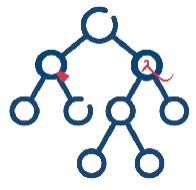
\includegraphics[height=1.0cm]{msca_logo.png}}%
    \end{center}

    \vspace{0.6cm}

    % Main title with Q logos on sides (with clickable links)
    \begin{center}
        \begin{minipage}{0.1\textwidth}
            \centering
            \href{https://quantlet.com}{
\includegraphics[height=1.1cm]{ql_logo.png}}
        \end{minipage}%
        \begin{minipage}{0.78\textwidth}
            \centering
            {\LARGE\bfseries\usebeamercolor[fg]{title}\inserttitle}

            \vspace{0.3cm}

            {\usebeamerfont{subtitle}\usebeamercolor[fg]{title}\insertsubtitle}
        \end{minipage}%
        \begin{minipage}{0.1\textwidth}
            \centering
            \href{https://quantinar.com}{
\includegraphics[height=1.1cm]{qr_logo.png}}
        \end{minipage}
    \end{center}

    \vspace{0.6cm}

    % Authors (left aligned)
    \hspace{0.5cm}{\usebeamerfont{author}\insertauthor}

    \vspace{0.3cm}

    % Institute/Affiliations (left aligned)
    \hspace{0.5cm}\begin{minipage}[t]{0.9\textwidth}
        \raggedright\small\insertinstitute
    \end{minipage}
}

%=============================================================================
% THEOREM ENVIRONMENTS
%=============================================================================
\theoremstyle{definition}
\setbeamertemplate{theorems}[numbered]
\ifdefined\atslang
\newtheorem{defn}{Definiție}
\newtheorem{thm}{Teoremă}
\newtheorem{prop}{Propoziție}
\newtheorem{rmk}{Observație}
\else
\newtheorem{defn}{Definition}
\newtheorem{thm}{Theorem}
\newtheorem{prop}{Proposition}
\newtheorem{rmk}{Remark}
\fi

%=============================================================================
% CENTRED MINIPAGE (no extra vertical space)
%=============================================================================
\newenvironment{cminipage}[1]{%
    \par\noindent\hfill\begin{minipage}{#1}\ignorespaces
}{%
    \end{minipage}\hfill\null\par
}

%=============================================================================
% CUSTOM COMMANDS
%=============================================================================
\newcommand{\E}{\mathbb{E}}
\newcommand{\Var}{\text{Var}}
\newcommand{\Cov}{\text{Cov}}
\newcommand{\Corr}{\text{Corr}}
\newcommand{\R}{\mathbb{R}}
\newcommand{\N}{\mathbb{N}}
\newcommand{\Z}{\mathbb{Z}}
\newcommand{\B}{\mathbf{B}}
\newcommand{\imark}{\textcolor{MainBlue}{\textbullet}}
\newcommand{\RMSE}{\text{RMSE}}
\newcommand{\MAE}{\text{MAE}}
\newcommand{\MAPE}{\text{MAPE}}

% Boldface vector/matrix commands (VAR, VECM, state space)
\newcommand{\bY}{\mathbf{Y}}
\newcommand{\bX}{\mathbf{X}}
\newcommand{\bA}{\mathbf{A}}
\newcommand{\bB}{\mathbf{B}}
\newcommand{\bepsilon}{\boldsymbol{\varepsilon}}
\newcommand{\bSigma}{\boldsymbol{\Sigma}}
\newcommand{\bPhi}{\boldsymbol{\Phi}}
\newcommand{\bGamma}{\boldsymbol{\Gamma}}
\newcommand{\bPi}{\boldsymbol{\Pi}}
\newcommand{\bc}{\mathbf{c}}
\newcommand{\balpha}{\boldsymbol{\alpha}}
\newcommand{\bbeta}{\boldsymbol{\beta}}
\newcommand{\bvarepsilon}{\boldsymbol{\varepsilon}}

% Seminar marks
\newcommand{\correct}{\textcolor{Forest}{\checkmark}}
\newcommand{\incorrect}{\textcolor{Crimson}{\texttimes}}
 se definește
%   \newcommand{\coursename}{Advanced Time Series Analysis and Forecasting}          (EN)
%   \newcommand{\coursename}{Analiza avansată a seriilor de timp și previziune}       (RO)  și  \def\atslang{ro}
% Fișierele .tex se află în EN/Courses, EN/Seminars, RO/Cursuri, RO/Seminarii (două niveluri sub rădăcină).
% Deck-urile sînt generate de latex/build_chapterN.py / build_seminarN.py (vezi latex/ats_build.py).

\documentclass[9pt, aspectratio=169, t]{beamer}
\providecommand{\coursename}{Advanced Time Series Analysis and Forecasting}

% Ensure content fits on slides
\setbeamersize{text margin left=8mm, text margin right=8mm}
% Smaller institute font (title page)
\setbeamerfont{institute}{size=\footnotesize}

%=============================================================================
% THEME AND STYLE CONFIGURATION
%=============================================================================
\usetheme{default}
% Using default theme for clean header/footer control

% Color Palette (matching Redispatch PDF)
\definecolor{MainBlue}{RGB}{26, 58, 110}
\definecolor{AccentBlue}{RGB}{26, 58, 110}
\definecolor{IDAred}{RGB}{205, 0, 0}
\definecolor{DarkGray}{RGB}{51, 51, 51}
\definecolor{MediumGray}{RGB}{128, 128, 128}
\definecolor{LightGray}{RGB}{248, 248, 248}
\definecolor{VeryLightGray}{RGB}{235, 235, 235}
\definecolor{KeynoteGray}{RGB}{218, 218, 218}
\definecolor{SectionGray}{RGB}{120, 120, 120}
\definecolor{FooterGray}{RGB}{100, 100, 100}
\definecolor{Crimson}{RGB}{220, 53, 69}
\definecolor{Forest}{RGB}{46, 125, 50}
\definecolor{Amber}{RGB}{181, 133, 63}
\definecolor{Orange}{RGB}{230, 126, 34}
\definecolor{Purple}{RGB}{142, 68, 173}

% Gradient background (exact Keynote 315° gradient: white to RGB 218,218,218)
\setbeamertemplate{background}{%
    \begin{tikzpicture}[remember picture, overlay]
        \shade[shading=axis, shading angle=315,
        top color=white, bottom color=KeynoteGray]
        (current page.south west) rectangle (current page.north east);
    \end{tikzpicture}%
}
% Fallback solid color for compatibility
\setbeamercolor{background canvas}{bg=}

\setbeamercolor{palette primary}{bg=MainBlue, fg=white}
\setbeamercolor{palette secondary}{bg=MainBlue!85, fg=white}
\setbeamercolor{palette tertiary}{bg=MainBlue!70, fg=white}
\setbeamercolor{structure}{fg=MainBlue}
\setbeamercolor{title}{fg=IDAred}
\setbeamercolor{frametitle}{fg=IDAred, bg=}
\setbeamercolor{block title}{bg=MainBlue, fg=white}
\setbeamercolor{block body}{bg=VeryLightGray, fg=DarkGray}
\setbeamercolor{block title alerted}{bg=Crimson, fg=white}
\setbeamercolor{block body alerted}{bg=Crimson!8, fg=DarkGray}
\setbeamercolor{block title example}{bg=Forest, fg=white}
\setbeamercolor{block body example}{bg=Forest!8, fg=DarkGray}
\setbeamercolor{item}{fg=MainBlue}

% Footer colors (override Madrid theme blue)
\setbeamercolor{author in head/foot}{fg=FooterGray, bg=}
\setbeamercolor{title in head/foot}{fg=FooterGray, bg=}
\setbeamercolor{date in head/foot}{fg=FooterGray, bg=}
\setbeamercolor{section in head/foot}{fg=FooterGray, bg=}
\setbeamercolor{subsection in head/foot}{fg=FooterGray, bg=}

% Bullet styles (apply everywhere including blocks)
\setbeamertemplate{itemize item}{\color{MainBlue}$\boxdot$}
\setbeamertemplate{itemize subitem}{\color{MainBlue}$\blacktriangleright$}
\setbeamertemplate{itemize subsubitem}{\color{MainBlue}\tiny$\bullet$}
\setbeamertemplate{itemize/enumerate body begin}{\normalsize}
\setbeamertemplate{itemize/enumerate subbody begin}{\normalsize}

% Item spacing - compact style
\setlength{\leftmargini}{10pt}       % Level 1: minimal indent
\setlength{\leftmarginii}{10pt}      % Level 2: minimal additional indent
% Compact list spacing (zero extra space before/after lists in blocks)
\makeatletter
\def\@listi{\leftmargin\leftmargini \topsep 0pt \parsep 0pt \itemsep 0pt}
\def\@listii{\leftmargin\leftmarginii \topsep 0pt \parsep 0pt \itemsep 0pt}
\makeatother

\setbeamertemplate{navigation symbols}{}

%=============================================================================
% CUSTOM HEADLINE
%=============================================================================
\setbeamertemplate{headline}{%
    \vskip10pt%
    \hbox to \paperwidth{%
        \hskip0.5cm%
        {\small\color{FooterGray}\renewcommand{\hyperlink}[2]{##2}\insertsectionhead}%
        \hfill%
        \textcolor{FooterGray}{\small\insertframenumber}%
        \hskip0.5cm%
    }%
    \vskip4pt%
    {\color{FooterGray}\hrule height 0.4pt}%
}

%=============================================================================
% CUSTOM FOOTER
%=============================================================================
\usepackage{fontawesome5}

\setbeamertemplate{footline}{%
    {\color{FooterGray}\hrule height 0.4pt}%
    \vskip4pt%
    \hbox to \paperwidth{%
        \hskip0.5cm%
        \textcolor{FooterGray}{\small\coursename}%
        \hfill%
        \raisebox{-0.1em}{%
            \begin{tikzpicture}[x=0.08em, y=0.08em, line width=0.4pt]
                \draw[FooterGray] (0,3) -- (1,4) -- (2,3.5) -- (3,5) -- (4,4) -- (5,6) -- (6,5.5) -- (7,4) -- (8,5) -- (9,7) -- (10,6) -- (11,5) -- (12,6.5) -- (13,8) -- (14,7) -- (15,6) -- (16,7.5) -- (17,9) -- (18,8) -- (19,7) -- (20,8.5) -- (21,10) -- (22,9) -- (23,8) -- (24,9.5);
            \end{tikzpicture}%
        }%
        \hskip0.5cm%
    }%
    \vskip6pt%
}

%=============================================================================
% PACKAGES
%=============================================================================
\usepackage[utf8]{inputenc}
\DeclareUnicodeCharacter{03B1}{\ensuremath{\alpha}}
\usepackage[T1]{fontenc}
\usepackage{amsmath, amssymb, amsthm}
\usepackage{mathtools}
\usepackage{bm}
\usepackage{tikz}
\usetikzlibrary{arrows.meta, positioning, shapes, calc, decorations.pathreplacing, shadings}
\usepackage{booktabs}
\usepackage{multirow}
\usepackage{array}
\usepackage{graphicx}
\usepackage{animate}
\usepackage{hyperref}
\usepackage{colortbl}
\usepackage{listings}
\lstset{language=Python, basicstyle=\ttfamily\scriptsize, keywordstyle=\color{MainBlue}\bfseries,
  commentstyle=\color{Forest}, stringstyle=\color{Crimson}, breaklines=true,
  frame=none, backgroundcolor=\color{VeryLightGray}, xleftmargin=2mm}
\hypersetup{colorlinks=true, linkcolor=MainBlue, urlcolor=MainBlue}
\graphicspath{{../../logos/}{../../charts/}{../../photos/}}
\usepackage{xcolor}
\hfuzz=2pt  % Suppress tiny overfull warnings (<2pt)
\vfuzz=2pt  % Suppress tiny vertical overfull warnings (<2pt)

%=============================================================================
% QUANTLET COMMANDS
%   \quantlet{<displayed name>}{<url>}       (generic)
%   \atsquantlet{Ch_05}{ATS_ch5_garch}       -> https://github.com/danpele/Advanced-Time-Series/tree/main/Quantlets/Ch_05/ATS_ch5_garch
%   \qlurl{<folder>} is defined per chapter by the generator (Quantlets/Ch_NN/<folder>)
%=============================================================================
\newcommand{\atsrepo}{https://github.com/danpele/Advanced-Time-Series}
\newcommand{\atsqlbase}{https://github.com/danpele/Advanced-Time-Series/tree/main/Quantlets}
\newcommand{\quantlet}[2]{%
    \hfill\href{#2}{%
        \raisebox{-0.15em}{
\includegraphics[height=0.7em]{ql_logo.png}}%
        \textcolor{MainBlue}{\tiny\ #1}%
    }%
}
\newcommand{\atsquantlet}[2]{\quantlet{\detokenize{#2}}{\atsqlbase/#1/#2}}

%=============================================================================
% NOTEBOOKS (Google Colab)
%   \colaburl{notebooks/EN/chapter5_seminar_notebook.ipynb} -> the Colab link of a file in the ATS repo
%   \nb: the chapter notebook (each seminar deck redefines it with \renewcommand)
%=============================================================================
\newcommand{\colaburl}[1]{https://colab.research.google.com/github/danpele/Advanced-Time-Series/blob/main/#1}
\newcommand{\nb}{https://colab.research.google.com/github/danpele/Advanced-Time-Series/tree/main/notebooks/EN}
\newcommand{\nbname}{notebooks/EN}

%=============================================================================
% SLIDE HELPERS (used by the generators; the same as in MFM)
%=============================================================================
% local font size for list bodies (the preamble forces \normalsize)
\newcommand{\itemsize}[1]{\setbeamertemplate{itemize/enumerate body begin}{#1}\setbeamertemplate{itemize/enumerate subbody begin}{#1}}
\newcommand{\intitle}[1]{{\hypersetup{urlcolor=white}#1}}   % white links inside coloured title bars
\newcommand{\imgcap}[1]{{\scriptsize #1}\\[0.5mm]}          % caption under a photo
\newcommand{\imgcredit}[2]{{\tiny\color{FooterGray}\href{#1}{#2}}}   % image credit: source URL, author/licence
\newcommand{\aiprompt}[1]{{\ttfamily\color{MainBlue}#1}}     % a prompt to an AI assistant

%=============================================================================
% SEMINARS: student version by default; the instructor wrapper *_solutions.tex sets \solutionstrue
%=============================================================================
\makeatletter\@ifundefined{ifsolutions}{\expandafter\newif\csname ifsolutions\endcsname}{}\makeatother
\newcommand{\solonly}[1]{\ifsolutions #1\fi}
\newcommand{\propsub}{\ifsolutions\else\framesubtitle{\ifdefined\atslang Rezolvarea se discută la seminar\else Solution discussed in class\fi}\fi}

%=============================================================================
% APPENDIX AND CHAPTER LINKS (latex/appendix_links.py writes the calls; it also re-declares these
% macros before \begin{document}, so the decks compile with or without this preamble block)
%=============================================================================
\providecommand{\atsapplink}[3]{\hypertarget{#2}{}\hyperlink{#1}{\beamergotobutton{#3}}}
\providecommand{\atsappback}[2]{\begin{tikzpicture}[remember picture,overlay]\node[anchor=south east] at ([xshift=-3mm,yshift=7mm]current page.south east){\hyperlink{#1}{\beamerreturnbutton{#2}}};\end{tikzpicture}}
\providecommand{\atschlink}[2]{\href{#1}{#2}}
\providecommand{\atschlinkt}[2]{\href{#1}{\usebeamercolor[fg]{frametitle}#2}}

%=============================================================================
% QUANTINAR COMMAND: link către un curs Quantinar (subiecte avansate)
%=============================================================================
\newcommand{\quantinar}[2]{%
    \href{#2}{%
        \raisebox{-0.15em}{
\includegraphics[height=0.8em]{qr_logo.png}}%
        \textcolor{MainBlue}{\scriptsize\ #1}%
    }%
}

%=============================================================================
% CUSTOM TITLE PAGE
%=============================================================================
\defbeamertemplate*{title page}{hybrid}[1][]
{
    \vspace{0.2cm}
    % Logos row - top header (with clickable links)
    \begin{center}
        \href{https://www.ase.ro}{
\includegraphics[height=1.0cm]{ase_logo.png}}\hspace{0.3cm}%
        \href{https://theida.net}{
\includegraphics[height=1.0cm]{ida_logo.png}}\hspace{0.3cm}%
        \href{https://blockchain-research-center.com}{
\includegraphics[height=1.0cm]{brc_logo.png}}\hspace{0.3cm}%
        \href{https://www.ai4efin.ase.ro}{
\includegraphics[height=1.0cm]{ai4efin_logo.png}}\hspace{0.3cm}%
        \href{https://ipe.ro/new}{
\includegraphics[height=1.0cm]{acad_logo.png}}\hspace{0.3cm}%
        \href{https://www.digital-finance-msca.com}{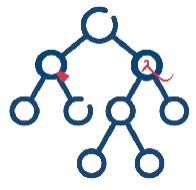
\includegraphics[height=1.0cm]{msca_logo.png}}%
    \end{center}

    \vspace{0.6cm}

    % Main title with Q logos on sides (with clickable links)
    \begin{center}
        \begin{minipage}{0.1\textwidth}
            \centering
            \href{https://quantlet.com}{
\includegraphics[height=1.1cm]{ql_logo.png}}
        \end{minipage}%
        \begin{minipage}{0.78\textwidth}
            \centering
            {\LARGE\bfseries\usebeamercolor[fg]{title}\inserttitle}

            \vspace{0.3cm}

            {\usebeamerfont{subtitle}\usebeamercolor[fg]{title}\insertsubtitle}
        \end{minipage}%
        \begin{minipage}{0.1\textwidth}
            \centering
            \href{https://quantinar.com}{
\includegraphics[height=1.1cm]{qr_logo.png}}
        \end{minipage}
    \end{center}

    \vspace{0.6cm}

    % Authors (left aligned)
    \hspace{0.5cm}{\usebeamerfont{author}\insertauthor}

    \vspace{0.3cm}

    % Institute/Affiliations (left aligned)
    \hspace{0.5cm}\begin{minipage}[t]{0.9\textwidth}
        \raggedright\small\insertinstitute
    \end{minipage}
}

%=============================================================================
% THEOREM ENVIRONMENTS
%=============================================================================
\theoremstyle{definition}
\setbeamertemplate{theorems}[numbered]
\ifdefined\atslang
\newtheorem{defn}{Definiție}
\newtheorem{thm}{Teoremă}
\newtheorem{prop}{Propoziție}
\newtheorem{rmk}{Observație}
\else
\newtheorem{defn}{Definition}
\newtheorem{thm}{Theorem}
\newtheorem{prop}{Proposition}
\newtheorem{rmk}{Remark}
\fi

%=============================================================================
% CENTRED MINIPAGE (no extra vertical space)
%=============================================================================
\newenvironment{cminipage}[1]{%
    \par\noindent\hfill\begin{minipage}{#1}\ignorespaces
}{%
    \end{minipage}\hfill\null\par
}

%=============================================================================
% CUSTOM COMMANDS
%=============================================================================
\newcommand{\E}{\mathbb{E}}
\newcommand{\Var}{\text{Var}}
\newcommand{\Cov}{\text{Cov}}
\newcommand{\Corr}{\text{Corr}}
\newcommand{\R}{\mathbb{R}}
\newcommand{\N}{\mathbb{N}}
\newcommand{\Z}{\mathbb{Z}}
\newcommand{\B}{\mathbf{B}}
\newcommand{\imark}{\textcolor{MainBlue}{\textbullet}}
\newcommand{\RMSE}{\text{RMSE}}
\newcommand{\MAE}{\text{MAE}}
\newcommand{\MAPE}{\text{MAPE}}

% Boldface vector/matrix commands (VAR, VECM, state space)
\newcommand{\bY}{\mathbf{Y}}
\newcommand{\bX}{\mathbf{X}}
\newcommand{\bA}{\mathbf{A}}
\newcommand{\bB}{\mathbf{B}}
\newcommand{\bepsilon}{\boldsymbol{\varepsilon}}
\newcommand{\bSigma}{\boldsymbol{\Sigma}}
\newcommand{\bPhi}{\boldsymbol{\Phi}}
\newcommand{\bGamma}{\boldsymbol{\Gamma}}
\newcommand{\bPi}{\boldsymbol{\Pi}}
\newcommand{\bc}{\mathbf{c}}
\newcommand{\balpha}{\boldsymbol{\alpha}}
\newcommand{\bbeta}{\boldsymbol{\beta}}
\newcommand{\bvarepsilon}{\boldsymbol{\varepsilon}}

% Seminar marks
\newcommand{\correct}{\textcolor{Forest}{\checkmark}}
\newcommand{\incorrect}{\textcolor{Crimson}{\texttimes}}
 se definește
%   \newcommand{\coursename}{Advanced Time Series Analysis and Forecasting}          (EN)
%   \newcommand{\coursename}{Analiza avansată a seriilor de timp și previziune}       (RO)  și  \def\atslang{ro}
% Fișierele .tex se află în EN/Courses, EN/Seminars, RO/Cursuri, RO/Seminarii (două niveluri sub rădăcină).
% Deck-urile sînt generate de latex/build_chapterN.py / build_seminarN.py (vezi latex/ats_build.py).

\documentclass[9pt, aspectratio=169, t]{beamer}
\providecommand{\coursename}{Advanced Time Series Analysis and Forecasting}

% Ensure content fits on slides
\setbeamersize{text margin left=8mm, text margin right=8mm}
% Smaller institute font (title page)
\setbeamerfont{institute}{size=\footnotesize}

%=============================================================================
% THEME AND STYLE CONFIGURATION
%=============================================================================
\usetheme{default}
% Using default theme for clean header/footer control

% Color Palette (matching Redispatch PDF)
\definecolor{MainBlue}{RGB}{26, 58, 110}
\definecolor{AccentBlue}{RGB}{26, 58, 110}
\definecolor{IDAred}{RGB}{205, 0, 0}
\definecolor{DarkGray}{RGB}{51, 51, 51}
\definecolor{MediumGray}{RGB}{128, 128, 128}
\definecolor{LightGray}{RGB}{248, 248, 248}
\definecolor{VeryLightGray}{RGB}{235, 235, 235}
\definecolor{KeynoteGray}{RGB}{218, 218, 218}
\definecolor{SectionGray}{RGB}{120, 120, 120}
\definecolor{FooterGray}{RGB}{100, 100, 100}
\definecolor{Crimson}{RGB}{220, 53, 69}
\definecolor{Forest}{RGB}{46, 125, 50}
\definecolor{Amber}{RGB}{181, 133, 63}
\definecolor{Orange}{RGB}{230, 126, 34}
\definecolor{Purple}{RGB}{142, 68, 173}

% Gradient background (exact Keynote 315° gradient: white to RGB 218,218,218)
\setbeamertemplate{background}{%
    \begin{tikzpicture}[remember picture, overlay]
        \shade[shading=axis, shading angle=315,
        top color=white, bottom color=KeynoteGray]
        (current page.south west) rectangle (current page.north east);
    \end{tikzpicture}%
}
% Fallback solid color for compatibility
\setbeamercolor{background canvas}{bg=}

\setbeamercolor{palette primary}{bg=MainBlue, fg=white}
\setbeamercolor{palette secondary}{bg=MainBlue!85, fg=white}
\setbeamercolor{palette tertiary}{bg=MainBlue!70, fg=white}
\setbeamercolor{structure}{fg=MainBlue}
\setbeamercolor{title}{fg=IDAred}
\setbeamercolor{frametitle}{fg=IDAred, bg=}
\setbeamercolor{block title}{bg=MainBlue, fg=white}
\setbeamercolor{block body}{bg=VeryLightGray, fg=DarkGray}
\setbeamercolor{block title alerted}{bg=Crimson, fg=white}
\setbeamercolor{block body alerted}{bg=Crimson!8, fg=DarkGray}
\setbeamercolor{block title example}{bg=Forest, fg=white}
\setbeamercolor{block body example}{bg=Forest!8, fg=DarkGray}
\setbeamercolor{item}{fg=MainBlue}

% Footer colors (override Madrid theme blue)
\setbeamercolor{author in head/foot}{fg=FooterGray, bg=}
\setbeamercolor{title in head/foot}{fg=FooterGray, bg=}
\setbeamercolor{date in head/foot}{fg=FooterGray, bg=}
\setbeamercolor{section in head/foot}{fg=FooterGray, bg=}
\setbeamercolor{subsection in head/foot}{fg=FooterGray, bg=}

% Bullet styles (apply everywhere including blocks)
\setbeamertemplate{itemize item}{\color{MainBlue}$\boxdot$}
\setbeamertemplate{itemize subitem}{\color{MainBlue}$\blacktriangleright$}
\setbeamertemplate{itemize subsubitem}{\color{MainBlue}\tiny$\bullet$}
\setbeamertemplate{itemize/enumerate body begin}{\normalsize}
\setbeamertemplate{itemize/enumerate subbody begin}{\normalsize}

% Item spacing - compact style
\setlength{\leftmargini}{10pt}       % Level 1: minimal indent
\setlength{\leftmarginii}{10pt}      % Level 2: minimal additional indent
% Compact list spacing (zero extra space before/after lists in blocks)
\makeatletter
\def\@listi{\leftmargin\leftmargini \topsep 0pt \parsep 0pt \itemsep 0pt}
\def\@listii{\leftmargin\leftmarginii \topsep 0pt \parsep 0pt \itemsep 0pt}
\makeatother

\setbeamertemplate{navigation symbols}{}

%=============================================================================
% CUSTOM HEADLINE
%=============================================================================
\setbeamertemplate{headline}{%
    \vskip10pt%
    \hbox to \paperwidth{%
        \hskip0.5cm%
        {\small\color{FooterGray}\renewcommand{\hyperlink}[2]{##2}\insertsectionhead}%
        \hfill%
        \textcolor{FooterGray}{\small\insertframenumber}%
        \hskip0.5cm%
    }%
    \vskip4pt%
    {\color{FooterGray}\hrule height 0.4pt}%
}

%=============================================================================
% CUSTOM FOOTER
%=============================================================================
\usepackage{fontawesome5}

\setbeamertemplate{footline}{%
    {\color{FooterGray}\hrule height 0.4pt}%
    \vskip4pt%
    \hbox to \paperwidth{%
        \hskip0.5cm%
        \textcolor{FooterGray}{\small\coursename}%
        \hfill%
        \raisebox{-0.1em}{%
            \begin{tikzpicture}[x=0.08em, y=0.08em, line width=0.4pt]
                \draw[FooterGray] (0,3) -- (1,4) -- (2,3.5) -- (3,5) -- (4,4) -- (5,6) -- (6,5.5) -- (7,4) -- (8,5) -- (9,7) -- (10,6) -- (11,5) -- (12,6.5) -- (13,8) -- (14,7) -- (15,6) -- (16,7.5) -- (17,9) -- (18,8) -- (19,7) -- (20,8.5) -- (21,10) -- (22,9) -- (23,8) -- (24,9.5);
            \end{tikzpicture}%
        }%
        \hskip0.5cm%
    }%
    \vskip6pt%
}

%=============================================================================
% PACKAGES
%=============================================================================
\usepackage[utf8]{inputenc}
\DeclareUnicodeCharacter{03B1}{\ensuremath{\alpha}}
\usepackage[T1]{fontenc}
\usepackage{amsmath, amssymb, amsthm}
\usepackage{mathtools}
\usepackage{bm}
\usepackage{tikz}
\usetikzlibrary{arrows.meta, positioning, shapes, calc, decorations.pathreplacing, shadings}
\usepackage{booktabs}
\usepackage{multirow}
\usepackage{array}
\usepackage{graphicx}
\usepackage{animate}
\usepackage{hyperref}
\usepackage{colortbl}
\usepackage{listings}
\lstset{language=Python, basicstyle=\ttfamily\scriptsize, keywordstyle=\color{MainBlue}\bfseries,
  commentstyle=\color{Forest}, stringstyle=\color{Crimson}, breaklines=true,
  frame=none, backgroundcolor=\color{VeryLightGray}, xleftmargin=2mm}
\hypersetup{colorlinks=true, linkcolor=MainBlue, urlcolor=MainBlue}
\graphicspath{{../../logos/}{../../charts/}{../../photos/}}
\usepackage{xcolor}
\hfuzz=2pt  % Suppress tiny overfull warnings (<2pt)
\vfuzz=2pt  % Suppress tiny vertical overfull warnings (<2pt)

%=============================================================================
% QUANTLET COMMANDS
%   \quantlet{<displayed name>}{<url>}       (generic)
%   \atsquantlet{Ch_05}{ATS_ch5_garch}       -> https://github.com/danpele/Advanced-Time-Series/tree/main/Quantlets/Ch_05/ATS_ch5_garch
%   \qlurl{<folder>} is defined per chapter by the generator (Quantlets/Ch_NN/<folder>)
%=============================================================================
\newcommand{\atsrepo}{https://github.com/danpele/Advanced-Time-Series}
\newcommand{\atsqlbase}{https://github.com/danpele/Advanced-Time-Series/tree/main/Quantlets}
\newcommand{\quantlet}[2]{%
    \hfill\href{#2}{%
        \raisebox{-0.15em}{
\includegraphics[height=0.7em]{ql_logo.png}}%
        \textcolor{MainBlue}{\tiny\ #1}%
    }%
}
\newcommand{\atsquantlet}[2]{\quantlet{\detokenize{#2}}{\atsqlbase/#1/#2}}

%=============================================================================
% NOTEBOOKS (Google Colab)
%   \colaburl{notebooks/EN/chapter5_seminar_notebook.ipynb} -> the Colab link of a file in the ATS repo
%   \nb: the chapter notebook (each seminar deck redefines it with \renewcommand)
%=============================================================================
\newcommand{\colaburl}[1]{https://colab.research.google.com/github/danpele/Advanced-Time-Series/blob/main/#1}
\newcommand{\nb}{https://colab.research.google.com/github/danpele/Advanced-Time-Series/tree/main/notebooks/EN}
\newcommand{\nbname}{notebooks/EN}

%=============================================================================
% SLIDE HELPERS (used by the generators; the same as in MFM)
%=============================================================================
% local font size for list bodies (the preamble forces \normalsize)
\newcommand{\itemsize}[1]{\setbeamertemplate{itemize/enumerate body begin}{#1}\setbeamertemplate{itemize/enumerate subbody begin}{#1}}
\newcommand{\intitle}[1]{{\hypersetup{urlcolor=white}#1}}   % white links inside coloured title bars
\newcommand{\imgcap}[1]{{\scriptsize #1}\\[0.5mm]}          % caption under a photo
\newcommand{\imgcredit}[2]{{\tiny\color{FooterGray}\href{#1}{#2}}}   % image credit: source URL, author/licence
\newcommand{\aiprompt}[1]{{\ttfamily\color{MainBlue}#1}}     % a prompt to an AI assistant

%=============================================================================
% SEMINARS: student version by default; the instructor wrapper *_solutions.tex sets \solutionstrue
%=============================================================================
\makeatletter\@ifundefined{ifsolutions}{\expandafter\newif\csname ifsolutions\endcsname}{}\makeatother
\newcommand{\solonly}[1]{\ifsolutions #1\fi}
\newcommand{\propsub}{\ifsolutions\else\framesubtitle{\ifdefined\atslang Rezolvarea se discută la seminar\else Solution discussed in class\fi}\fi}

%=============================================================================
% APPENDIX AND CHAPTER LINKS (latex/appendix_links.py writes the calls; it also re-declares these
% macros before \begin{document}, so the decks compile with or without this preamble block)
%=============================================================================
\providecommand{\atsapplink}[3]{\hypertarget{#2}{}\hyperlink{#1}{\beamergotobutton{#3}}}
\providecommand{\atsappback}[2]{\begin{tikzpicture}[remember picture,overlay]\node[anchor=south east] at ([xshift=-3mm,yshift=7mm]current page.south east){\hyperlink{#1}{\beamerreturnbutton{#2}}};\end{tikzpicture}}
\providecommand{\atschlink}[2]{\href{#1}{#2}}
\providecommand{\atschlinkt}[2]{\href{#1}{\usebeamercolor[fg]{frametitle}#2}}

%=============================================================================
% QUANTINAR COMMAND: link către un curs Quantinar (subiecte avansate)
%=============================================================================
\newcommand{\quantinar}[2]{%
    \href{#2}{%
        \raisebox{-0.15em}{
\includegraphics[height=0.8em]{qr_logo.png}}%
        \textcolor{MainBlue}{\scriptsize\ #1}%
    }%
}

%=============================================================================
% CUSTOM TITLE PAGE
%=============================================================================
\defbeamertemplate*{title page}{hybrid}[1][]
{
    \vspace{0.2cm}
    % Logos row - top header (with clickable links)
    \begin{center}
        \href{https://www.ase.ro}{
\includegraphics[height=1.0cm]{ase_logo.png}}\hspace{0.3cm}%
        \href{https://theida.net}{
\includegraphics[height=1.0cm]{ida_logo.png}}\hspace{0.3cm}%
        \href{https://blockchain-research-center.com}{
\includegraphics[height=1.0cm]{brc_logo.png}}\hspace{0.3cm}%
        \href{https://www.ai4efin.ase.ro}{
\includegraphics[height=1.0cm]{ai4efin_logo.png}}\hspace{0.3cm}%
        \href{https://ipe.ro/new}{
\includegraphics[height=1.0cm]{acad_logo.png}}\hspace{0.3cm}%
        \href{https://www.digital-finance-msca.com}{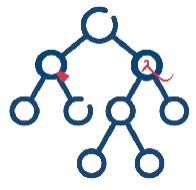
\includegraphics[height=1.0cm]{msca_logo.png}}%
    \end{center}

    \vspace{0.6cm}

    % Main title with Q logos on sides (with clickable links)
    \begin{center}
        \begin{minipage}{0.1\textwidth}
            \centering
            \href{https://quantlet.com}{
\includegraphics[height=1.1cm]{ql_logo.png}}
        \end{minipage}%
        \begin{minipage}{0.78\textwidth}
            \centering
            {\LARGE\bfseries\usebeamercolor[fg]{title}\inserttitle}

            \vspace{0.3cm}

            {\usebeamerfont{subtitle}\usebeamercolor[fg]{title}\insertsubtitle}
        \end{minipage}%
        \begin{minipage}{0.1\textwidth}
            \centering
            \href{https://quantinar.com}{
\includegraphics[height=1.1cm]{qr_logo.png}}
        \end{minipage}
    \end{center}

    \vspace{0.6cm}

    % Authors (left aligned)
    \hspace{0.5cm}{\usebeamerfont{author}\insertauthor}

    \vspace{0.3cm}

    % Institute/Affiliations (left aligned)
    \hspace{0.5cm}\begin{minipage}[t]{0.9\textwidth}
        \raggedright\small\insertinstitute
    \end{minipage}
}

%=============================================================================
% THEOREM ENVIRONMENTS
%=============================================================================
\theoremstyle{definition}
\setbeamertemplate{theorems}[numbered]
\ifdefined\atslang
\newtheorem{defn}{Definiție}
\newtheorem{thm}{Teoremă}
\newtheorem{prop}{Propoziție}
\newtheorem{rmk}{Observație}
\else
\newtheorem{defn}{Definition}
\newtheorem{thm}{Theorem}
\newtheorem{prop}{Proposition}
\newtheorem{rmk}{Remark}
\fi

%=============================================================================
% CENTRED MINIPAGE (no extra vertical space)
%=============================================================================
\newenvironment{cminipage}[1]{%
    \par\noindent\hfill\begin{minipage}{#1}\ignorespaces
}{%
    \end{minipage}\hfill\null\par
}

%=============================================================================
% CUSTOM COMMANDS
%=============================================================================
\newcommand{\E}{\mathbb{E}}
\newcommand{\Var}{\text{Var}}
\newcommand{\Cov}{\text{Cov}}
\newcommand{\Corr}{\text{Corr}}
\newcommand{\R}{\mathbb{R}}
\newcommand{\N}{\mathbb{N}}
\newcommand{\Z}{\mathbb{Z}}
\newcommand{\B}{\mathbf{B}}
\newcommand{\imark}{\textcolor{MainBlue}{\textbullet}}
\newcommand{\RMSE}{\text{RMSE}}
\newcommand{\MAE}{\text{MAE}}
\newcommand{\MAPE}{\text{MAPE}}

% Boldface vector/matrix commands (VAR, VECM, state space)
\newcommand{\bY}{\mathbf{Y}}
\newcommand{\bX}{\mathbf{X}}
\newcommand{\bA}{\mathbf{A}}
\newcommand{\bB}{\mathbf{B}}
\newcommand{\bepsilon}{\boldsymbol{\varepsilon}}
\newcommand{\bSigma}{\boldsymbol{\Sigma}}
\newcommand{\bPhi}{\boldsymbol{\Phi}}
\newcommand{\bGamma}{\boldsymbol{\Gamma}}
\newcommand{\bPi}{\boldsymbol{\Pi}}
\newcommand{\bc}{\mathbf{c}}
\newcommand{\balpha}{\boldsymbol{\alpha}}
\newcommand{\bbeta}{\boldsymbol{\beta}}
\newcommand{\bvarepsilon}{\boldsymbol{\varepsilon}}

% Seminar marks
\newcommand{\correct}{\textcolor{Forest}{\checkmark}}
\newcommand{\incorrect}{\textcolor{Crimson}{\texttimes}}


\newcommand{\qlurl}[1]{https://github.com/danpele/Advanced-Time-Series/tree/main/Quantlets/Ch_05/#1}

% Clickable citations (DOIs verified via Crossref)
\newcommand{\refADS}{\href{https://doi.org/10.1198/jbes.2009.07205}{Aruoba, Diebold and Scotti (2009)}}
\newcommand{\refAGK}{\href{https://doi.org/10.1080/07350015.2013.767199}{Andreou, Ghysels and Kourtellos (2013)}}
\newcommand{\refBBE}{\href{https://doi.org/10.1162/0033553053327452}{Bernanke, Boivin and Eliasz (2005)}}
\newcommand{\refBGMR}{\href{https://doi.org/10.1016/B978-0-444-53683-9.00004-9}{Bańbura, Giannone, Modugno and Reichlin (2013)}}
\newcommand{\refBGP}{\href{https://doi.org/10.1016/S0169-2070(03)00067-0}{Baffigi, Golinelli and Parigi (2004)}}
\newcommand{\refBGR}{\href{https://doi.org/10.1002/jae.1137}{Bańbura, Giannone and Reichlin (2010)}}
\newcommand{\refBM}{\href{https://doi.org/10.1002/jae.2306}{Bańbura and Modugno (2014)}}
\newcommand{\refBN}{\href{https://doi.org/10.1111/1468-0262.00273}{Bai and Ng (2002)}}
\newcommand{\refBai}{\href{https://doi.org/10.1111/1468-0262.00392}{Bai (2003)}}
\newcommand{\refBDA}{\href{https://doi.org/10.1201/b16018}{Gelman et al.\ (2013)}}
\newcommand{\refCCMa}{\href{https://doi.org/10.1080/07350015.2015.1040116}{Carriero, Clark and Marcellino (2016)}}
\newcommand{\refCCMb}{\href{https://doi.org/10.1016/j.jeconom.2019.04.024}{Carriero, Clark and Marcellino (2019)}}
\newcommand{\refCG}{\href{https://doi.org/10.1198/073500108000000015}{Clements and Galvão (2008)}}
\newcommand{\refChan}{\href{https://doi.org/10.1007/978-3-030-31150-6_4}{Chan (2020)}}
\newcommand{\refClark}{\href{https://doi.org/10.1198/jbes.2010.09248}{Clark (2011)}}
\newcommand{\refCR}{\href{https://doi.org/10.2307/1912275}{Chamberlain and Rothschild (1983)}}
\newcommand{\refCS}{\href{https://doi.org/10.1016/S0304-4076(01)00072-0}{Croushore and Stark (2001)}}
\newcommand{\refDGRa}{\href{https://doi.org/10.1016/j.jeconom.2008.08.011}{De Mol, Giannone and Reichlin (2008)}}
\newcommand{\refDGRb}{\href{https://doi.org/10.1016/j.jeconom.2011.02.012}{Doz, Giannone and Reichlin (2011)}}
\newcommand{\refDGRc}{\href{https://doi.org/10.1162/REST_a_00225}{Doz, Giannone and Reichlin (2012)}}
\newcommand{\refDK}{\href{https://doi.org/10.1093/acprof:oso/9780199641178.001.0001}{Durbin and Koopman (2012)}}
\newcommand{\refDLS}{\href{https://doi.org/10.1080/07474938408800053}{Doan, Litterman and Sims (1984)}}
\newcommand{\refFHLR}{\href{https://doi.org/10.1162/003465300559037}{Forni, Hallin, Lippi and Reichlin (2000)}}
\newcommand{\refFMS}{\href{https://doi.org/10.1111/rssa.12043}{Foroni, Marcellino and Schumacher (2015)}}
\newcommand{\refGG}{\href{https://doi.org/10.1109/TPAMI.1984.4767596}{Geman and Geman (1984)}}
\newcommand{\refGh}{\href{https://doi.org/10.1016/j.jeconom.2016.04.008}{Ghysels (2016)}}
\newcommand{\refGLP}{\href{https://doi.org/10.1162/REST_a_00483}{Giannone, Lenza and Primiceri (2015)}}
\newcommand{\refGLPb}{\href{https://doi.org/10.3982/ECTA17842}{Giannone, Lenza and Primiceri (2021)}}
\newcommand{\refGR}{\href{https://doi.org/10.1214/ss/1177011136}{Gelman and Rubin (1992)}}
\newcommand{\refGRS}{\href{https://doi.org/10.1016/j.jmoneco.2008.05.010}{Giannone, Reichlin and Small (2008)}}
\newcommand{\refGS}{\href{https://doi.org/10.1080/01621459.1990.10476213}{Gelfand and Smith (1990)}}
\newcommand{\refGSV}{\href{https://doi.org/10.1016/j.jeconom.2005.01.004}{Ghysels, Santa-Clara and Valkanov (2006)}}
\newcommand{\refGSVb}{\href{https://doi.org/10.1080/07474930600972467}{Ghysels, Sinko and Valkanov (2007)}}
\newcommand{\refHam}{\href{https://doi.org/10.2307/j.ctv14jx6sm}{Hamilton (1994)}}
\newcommand{\refKarl}{\href{https://doi.org/10.1016/B978-0-444-62731-5.00015-4}{Karlsson (2013)}}
\newcommand{\refKK}{\href{https://doi.org/10.1002/(SICI)1099-1255(199703)12:2\%3C99::AID-JAE429\%3E3.0.CO;2-A}{Kadiyala and Karlsson (1997)}}
\newcommand{\refKL}{\href{https://doi.org/10.1017/9781108164818}{Kilian and Lütkepohl (2017)}}
\newcommand{\refKoKo}{\href{https://doi.org/10.1561/0800000013}{Koop and Korobilis (2010)}}
\newcommand{\refKoop}{\href{https://doi.org/10.1002/jae.1270}{Koop (2013)}}
\newcommand{\refKR}{\href{https://doi.org/10.1080/01621459.1995.10476572}{Kass and Raftery (1995)}}
\newcommand{\refLit}{\href{https://doi.org/10.1080/07350015.1986.10509491}{Litterman (1986)}}
\newcommand{\refLP}{\href{https://doi.org/10.1002/jae.2895}{Lenza and Primiceri (2022)}}
\newcommand{\refMM}{\href{https://doi.org/10.1002/jae.695}{Mariano and Murasawa (2003)}}
\newcommand{\refMN}{\href{https://doi.org/10.1080/07350015.2015.1086655}{McCracken and Ng (2016)}}
\newcommand{\refPet}{\href{https://doi.org/10.1016/j.ijforecast.2021.11.001}{Petropoulos et al.\ (2022)}}
\newcommand{\refPrim}{\href{https://doi.org/10.1111/j.1467-937X.2005.00353.x}{Primiceri (2005)}}
\newcommand{\refSims}{\href{https://www.nber.org/books-and-chapters/business-cycles-indicators-and-forecasting/nine-variable-probabilistic-macroeconomic-forecasting-model}{Sims (1993)}}
\newcommand{\refSS}{\href{https://doi.org/10.1080/07350015.2014.954707}{Schorfheide and Song (2015)}}
\newcommand{\refSWa}{\href{https://doi.org/10.1198/016214502388618960}{Stock and Watson (2002a)}}
\newcommand{\refSWb}{\href{https://doi.org/10.1198/073500102317351921}{Stock and Watson (2002b)}}
\newcommand{\refSWc}{\href{https://doi.org/10.1016/bs.hesmac.2016.04.002}{Stock and Watson (2016)}}
\newcommand{\refSWd}{\href{https://doi.org/10.1086/654119}{Stock and Watson (1989)}}
\newcommand{\refSZ}{\href{https://doi.org/10.2307/2527347}{Sims and Zha (1998)}}
\newcommand{\refVGS}{\href{https://doi.org/10.1214/20-BA1221}{Vehtari et al.\ (2021)}}

\title[Advanced Time Series Analysis and Forecasting]{Advanced Time Series Analysis and Forecasting}
\subtitle{Chapter 5: Bayesian VAR, factor models and nowcasting}
\author[D.T. Pele]{Daniel Traian PELE}
\institute{Bucharest University of Economic Studies\\
IDA Institute Digital Assets\\
Blockchain Research Center\\
AI4EFin Artificial Intelligence for Energy Finance\\
Romanian Academy, Institute for Economic Forecasting\\
MSCA Digital Finance}
\date{}

%=============================================================================
\providecommand{\atsapplink}[3]{\hypertarget{#2}{}\hyperlink{#1}{\beamergotobutton{#3}}}  % APPLINKS-MACROS
\providecommand{\atsappback}[2]{\begin{tikzpicture}[remember picture,overlay]\node[anchor=south east] at ([xshift=-3mm,yshift=7mm]current page.south east){\hyperlink{#1}{\beamerreturnbutton{#2}}};\end{tikzpicture}}  % APPLINKS-MACROS
\providecommand{\atschlink}[2]{\href{#1}{#2}}  % APPLINKS-MACROS
\providecommand{\atschlinkt}[2]{\href{#1}{\usebeamercolor[fg]{frametitle}#2}}  % APPLINKS-MACROS
\begin{document}
%=============================================================================

{
\setbeamertemplate{headline}{}
\setbeamertemplate{footline}{}
\begin{frame}[noframenumbering]
    \titlepage
\end{frame}
}
% BEGIN-ACRONYMS (generat de latex/acronyms.py; nu editati manual)
\begin{frame}{Acronyms used in this material (1/2)}
\setbeamertemplate{itemize/enumerate body begin}{\tiny}
\begin{columns}[T]
\begin{column}{0.49\textwidth}
\begin{itemize}\setlength{\itemsep}{0pt}
    \item \textbf{ADL-MIDAS}: Autoregressive Distributed Lag MIDAS
    \item \textbf{AI}: Artificial Intelligence
    \item \textbf{AR}: AutoRegressive (model); in event studies: Abnormal Return
    \item \textbf{BGR}: Bańbura–Giannone–Reichlin (large Bayesian VARs, 2010)
    \item \textbf{BIC}: Bayesian Information Criterion
    \item \textbf{BVAR}: Bayesian Vector AutoRegression
    \item \textbf{CPI}: Consumer Price Index
    \item \textbf{CUMFNS}: Capacity utilisation, manufacturing (FRED series code)
    \item \textbf{DFM}: Dynamic Factor Model
    \item \textbf{DI}: Diffusion Index (forecast)
    \item \textbf{DI-AR}: Diffusion Index forecast with AutoRegressive lags
    \item \textbf{EM}: Expectation–Maximisation (algorithm)
    \item \textbf{EMPL}: employment (total private payrolls)
\end{itemize}
\end{column}
\begin{column}{0.49\textwidth}
\begin{itemize}\setlength{\itemsep}{0pt}
    \item \textbf{ESI}: Economic Sentiment Indicator (European Commission)
    \item \textbf{ESS}: Effective Sample Size
    \item \textbf{FAVAR}: Factor-Augmented Vector AutoRegression
    \item \textbf{FFR}: Federal Funds Rate
    \item \textbf{FRED}: Federal Reserve Economic Data
    \item \textbf{FRED-MD}: FRED Monthly Database for macroeconomic research (McCracken–Ng)
    \item \textbf{GDP}: Gross Domestic Product
    \item \textbf{GLP}: Giannone–Lenza–Primiceri (hierarchical prior selection, 2015)
    \item \textbf{INS}: Institutul Național de Statistică (the National Institute of Statistics (Romania))
    \item \textbf{IP}: Industrial Production
    \item \textbf{LARGE}: the large system of BGR (all series observed over the sample)
    \item \textbf{LLM}: Large Language Model
    \item \textbf{MCMC}: Markov Chain Monte Carlo
\end{itemize}
\end{column}
\end{columns}
\end{frame}
\begin{frame}{Acronyms used in this material (2/2)}
\setbeamertemplate{itemize/enumerate body begin}{\tiny}
\begin{columns}[T]
\begin{column}{0.49\textwidth}
\begin{itemize}\setlength{\itemsep}{0pt}
    \item \textbf{MEDIUM}: the 20-variable system of BGR
    \item \textbf{MIDAS}: MIxed DAta Sampling (regression)
    \item \textbf{ML}: Machine Learning
    \item \textbf{MSE}: Mean Squared Error
    \item \textbf{MSFE}: Mean Squared Forecast Error
    \item \textbf{NBER}: National Bureau of Economic Research
    \item \textbf{NIW}: Normal–inverse-Wishart (prior)
    \item \textbf{NLS}: Nonlinear Least Squares
    \item \textbf{OLS}: Ordinary Least Squares
    \item \textbf{PCA}: Principal Component Analysis
    \item \textbf{RMSE}: Root Mean Squared Error
    \item \textbf{SE}: Standard Error
    \item \textbf{SMALL}: the 3-variable system of BGR (employment, CPI, federal funds rate)
\end{itemize}
\end{column}
\begin{column}{0.49\textwidth}
\begin{itemize}\setlength{\itemsep}{0pt}
    \item \textbf{TSA}: Time Series Analysis
    \item \textbf{UNRATE}: Unemployment Rate (FRED series code)
    \item \textbf{US}: United States
    \item \textbf{USREC}: NBER recession indicator (FRED series code)
    \item \textbf{VAR}: Vector AutoRegression
\end{itemize}
\end{column}
\end{columns}
\end{frame}
% END-ACRONYMS

\begin{frame}{Today's question and route}
\itemsize{\small}
\begin{itemize}
    \item \textbf{Question}: how do we forecast and analyse an economy described by a hundred series, some of them published monthly and late, others quarterly?
    \begin{itemize}
        \item an unrestricted VAR with 100 variables and 13 lags has more than 130\,000 coefficients: the data alone cannot pin them down
    \end{itemize}
    \item \textbf{Route} of the chapter
    \begin{itemize}
        \item the curse of dimensionality; Bayesian inference at the depth we need (conjugacy, Gibbs sampling, MCMC diagnostics)
        \item Minnesota and Normal--inverse-Wishart priors, dummy observations, shrinkage chosen by the marginal likelihood, large BVARs
        \item factor models: principal components, the number of factors, diffusion indexes, FAVAR, dynamic factor models
        \item mixed frequencies and nowcasting: bridge equations, MIDAS, the Kalman filter with a ragged edge, news; Romanian GDP
    \end{itemize}
    \item We build on \atschlink{https://danpele.github.io/Time-Series-Analysis/EN/Courses/chapter6_var_models_granger_causality.pdf}{TSA, Chapter 6} (VAR), \atschlink{https://danpele.github.io/Time-Series-Analysis/EN/Courses/chapter10_state_space_kalman_markov_switching.pdf}{TSA, Chapter 10} (Kalman filter) and \atschlink{https://danpele.github.io/Advanced-Time-Series/EN/Courses/chapter3_structural_var_local_projections.pdf}{Chapter 3} (structural VAR); Seminar 5 comes before this lecture
\end{itemize}
\end{frame}

\begin{frame}{Learning outcomes}
\itemsize{\small}
\begin{itemize}
    \item Derive conjugate posteriors, run a Gibbs sampler and judge its convergence with trace plots, effective sample size and $\widehat R$
    \item Write the Minnesota prior in natural conjugate form and with dummy observations, and explain each hyperparameter
    \item Choose the tightness of a large BVAR by the marginal likelihood or by the in-sample fit rule, and evaluate the forecasts out of sample
    \item Estimate approximate factor models by principal components, select the number of factors and build diffusion-index forecasts and a FAVAR
    \item Nowcast quarterly GDP from monthly data with bridge equations, MIDAS and a dynamic factor model, and decompose each revision into news
\end{itemize}
\end{frame}

\begin{frame}{Reading, data and tools}
\itemsize{\small}
\begin{itemize}
    \item Backbone: \refKL, Ch.~5 (Bayesian VAR) and Ch.~16 (large VARs, factors); \refKarl; \refSWc
    \begin{itemize}
        \item Bayesian background: \refBDA; state space: \refDK; nowcasting survey: \refBGMR
    \end{itemize}
    \item Python Quantlets of this chapter: \href{https://github.com/danpele/Advanced-Time-Series/tree/main/Quantlets/Ch_05}{Quantlets/Ch\_05}
    \begin{itemize}
        \item Minnesota and Normal--inverse-Wishart BVAR, marginal likelihood, PCA with EM, Bai--Ng, FAVAR, Kalman filter and news written in \texttt{numpy}
        \item comparison packages: \texttt{statsmodels} (DynamicFactorMQ, EM estimation of the nowcasting model) and \texttt{bvar} of the Bank of England (GLP hyperparameters)
    \end{itemize}
    \item Lecture notebook: \href{\colaburl{notebooks/EN/chapter5_lecture_notebook.ipynb}}{open in Google Colab}
\end{itemize}
\end{frame}

\begin{frame}{Data used in this chapter}
\itemsize{\footnotesize}
\begin{center}
\scriptsize
\begin{tabular}{>{\raggedright\arraybackslash}p{5.0cm}>{\raggedright\arraybackslash}p{4.6cm}>{\raggedright\arraybackslash}p{2.4cm}}
\toprule
\textbf{Series} & \textbf{Source} & \textbf{Use} \\
\midrule
117 US monthly series in the FRED-MD format (output, labour, housing, orders, money, rates, prices), 1960:1--2026:7 & FRED (St.~Louis Fed), one CSV per series; FRED-MD transformation codes \refMN{} & BVAR, factors, FAVAR \\
NBER recession dates; US capacity utilisation, unemployment rate & FRED (USREC, CUMFNS, UNRATE) & charts, Gibbs \\
Romania: IP, retail trade, construction, unemployment, six confidence indicators (11 monthly series); euro-area IP & Eurostat (sts\_inpr\_m, sts\_trtu\_m, sts\_copr\_m, une\_rt\_m, ei\_bssi\_m\_r2) & nowcasting \\
Romanian real GDP, quarterly, seasonally and calendar adjusted & Eurostat (namq\_10\_gdp) & target \\
\bottomrule
\end{tabular}
\end{center}
\begin{itemize}
    \item All sources are public and need no account or key; FRED-MD codes: 1 level, 2 difference, 4 log, 5 log difference, 6 second log difference
    \item October 2025: the US household survey and CPI were not collected (federal shutdown); the isolated missing month is interpolated
\end{itemize}
\end{frame}

\begin{frame}{Shrinkage was born in Minneapolis}
\itemsize{\footnotesize}
\begin{columns}[T]
\begin{column}{0.40\textwidth}
\centering
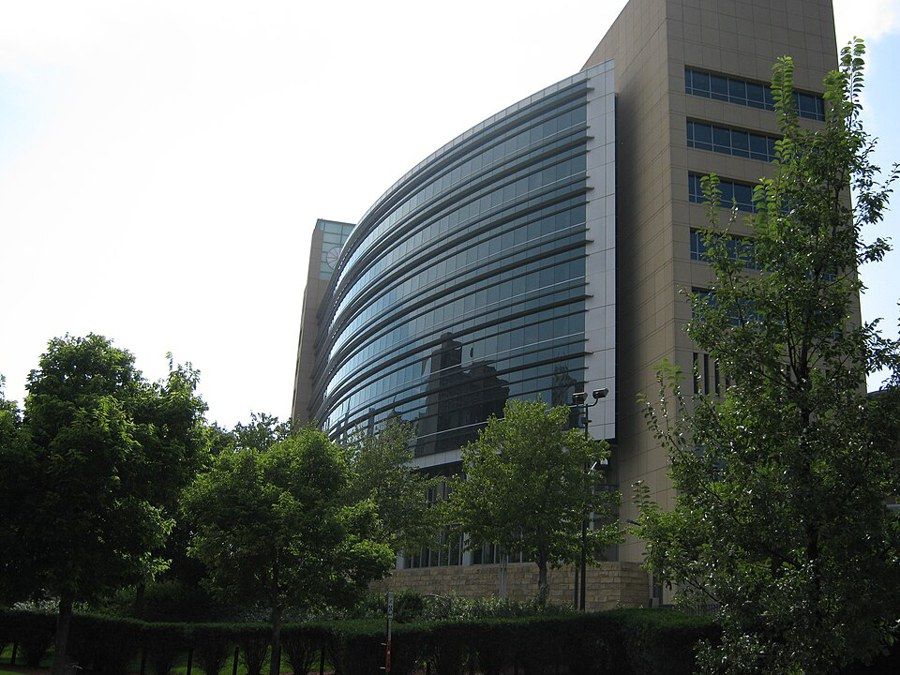
\includegraphics[height=0.34\textheight]{ch5_minneapolis_fed_2010.jpg}\\[1mm]
\imgcap{Federal Reserve Bank of Minneapolis, 2010}
\imgcredit{https://commons.wikimedia.org/wiki/File:Federal_Reserve_Bank_of_Minneapolis_building_2.jpg}{Photo: Innotata (2010); CC BY-SA 3.0; Wikimedia Commons}
\end{column}
\begin{column}{0.58\textwidth}
\begin{itemize}
    \item Early 1980s: Litterman forecasts with Bayesian VARs at the Minneapolis Fed \refLit; the ``Minnesota prior''
    \begin{itemize}
        \item \refDLS: sum-of-coefficients and conditional projections; \refSims, \refSZ: dummy initial observations
    \end{itemize}
    \item 1989--2002: dynamic factor indexes \refSWd, generalised dynamic factors \refFHLR, diffusion indexes \refSWa
    \item 2005--2015: FAVAR \refBBE, nowcasting \refGRS, large BVARs \refBGR, hierarchical priors \refGLP
    \item One idea throughout: when parameters outnumber observations, add information (a prior) or reduce dimension (factors)
\end{itemize}
\end{column}
\end{columns}
\end{frame}


%=============================================================================
\section{The curse of dimensionality}
%=============================================================================

\begin{frame}{Counting parameters}
\itemsize{\small}
\begin{itemize}
    \item VAR($p$) in $n$ variables: $k = np + 1$ regressors per equation, $n k$ slope coefficients and $n(n + 1)/2$ covariances
    \begin{itemize}
        \item $n = 3$, $p = 13$: $k = 40$; $n = 20$: $k = 261$; $n = 102$: $k = 1\,327$ per equation
        \item a 10-year window has $T = 120$ months: with $k > T$, OLS does not exist ($X'X$ is singular)
    \end{itemize}
    \item Even with $k < T$, the estimation error grows with $k/T$: one-step MSE $\approx \sigma^2(1 + k/T)$ for a correctly specified regression
    \begin{itemize}
        \item overfitting: in-sample fit improves, out-of-sample accuracy deteriorates
    \end{itemize}
    \item Three remedies: (i) shrinkage (Bayesian priors, ridge, LASSO); (ii) dimension reduction (factors); (iii) variable selection
\end{itemize}
\end{frame}

\begin{frame}{Simulation: OLS VAR against a Minnesota BVAR}
\itemsize{\footnotesize}
\begin{center}
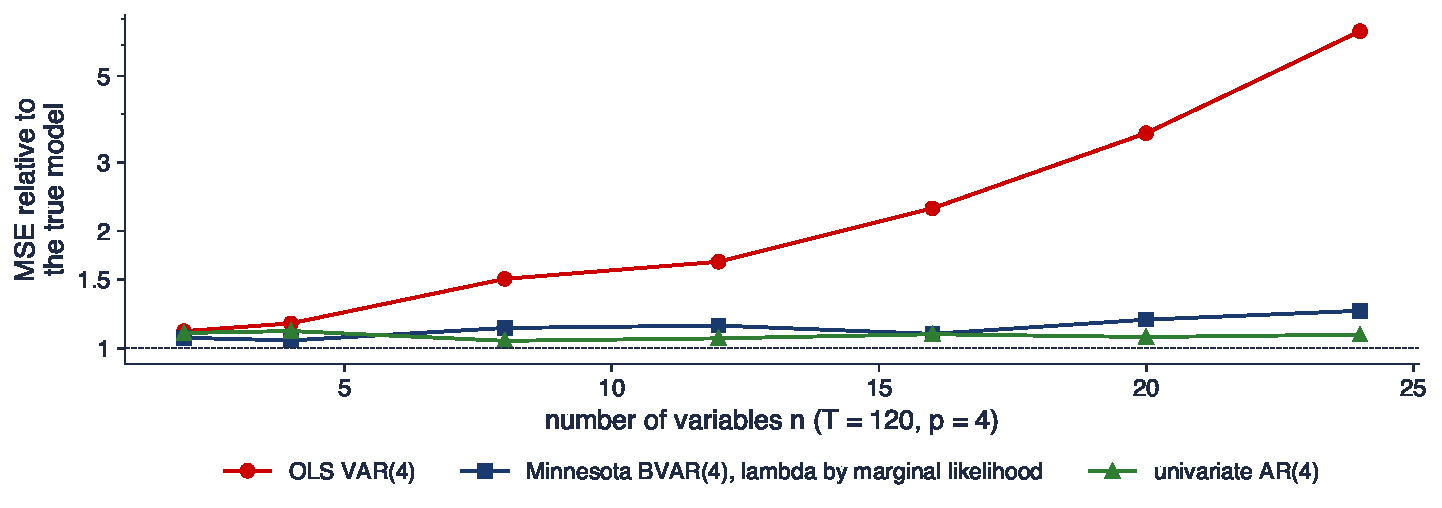
\includegraphics[width=0.97\textwidth,height=0.5\textheight,keepaspectratio]{ats_ch5_curse.pdf}
\end{center}
\vspace{-0.25cm}
\begin{itemize}
    \item True model: stationary VAR(1) $A = 0.5I + (0.3/n)\mathbf{1}\mathbf{1}'$; estimated VAR(4), $T = 120$; one-step MSE of variable 1 relative to the true model; 200 replications
\end{itemize}
\quantlet{ATS\_ch5\_bvar}{\qlurl{ATS_ch5_bvar}}
\end{frame}

\begin{frame}{Interpreting the simulation}
\itemsize{\small}
\begin{itemize}
    \item OLS: the relative MSE climbs to 6.52 at $n = 24$ ($k = 97$ regressors for 116 observations)
    \item BVAR: 1.25 at $n = 24$; the tightness chosen by the marginal likelihood falls from 0.31 ($n = 2$) to 0.14 ($n = 24$)
    \item A univariate AR(4) stays near 1.08: the cross-variable information is real but small, and OLS spends it on noise
    \item The larger the system, the tighter the prior should be: the theme of the whole chapter \refDGRa
\end{itemize}
\end{frame}

\begin{frame}{Recap: The curse of dimensionality}
\itemsize{\small}
\begin{itemize}
    \item Parameters grow with $n^2p$; observations do not
    \item Shrinkage trades a small bias for a large reduction of variance
    \item Factors summarise many series by a few common components
\end{itemize}
\end{frame}


%=============================================================================
\section{Bayesian inference: what we need}
%=============================================================================

\begin{frame}{Prior, likelihood, posterior}
\itemsize{\footnotesize}
\begin{columns}[T]
\begin{column}{0.34\textwidth}
\centering
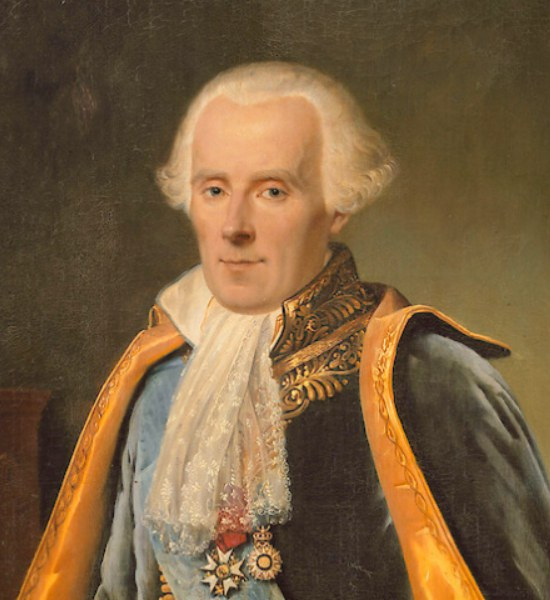
\includegraphics[height=0.36\textheight]{ch5_laplace_guerin_1838.jpg}\\[1mm]
\imgcap{Pierre-Simon Laplace, who developed inverse probability}
\imgcredit{https://commons.wikimedia.org/wiki/File:Pierre-Simon_Laplace.jpg}{Portrait: Paulin Guérin (1838); public domain; Wikimedia Commons}
\end{column}
\begin{column}{0.64\textwidth}
\begin{itemize}
    \item Bayes: $p(\theta\mid y) = p(y\mid\theta)p(\theta)/p(y)$, with $p(y) = \int p(y\mid\theta)p(\theta)\,d\theta$
    \begin{itemize}
        \item $\theta$: the parameters; $y$: the data; $p(\theta)$: \textbf{prior}; $p(y\mid\theta)$: likelihood; $p(\theta\mid y)$: \textbf{posterior}
        \item $p(y)$: \textbf{marginal likelihood}, the evidence for the model and its prior
    \end{itemize}
    \item Conjugacy: prior and posterior in the same family, so the posterior has a closed form
    \begin{itemize}
        \item Normal mean with known variance: Normal; regression coefficients and variance: Normal--inverse-gamma
    \end{itemize}
    \item Point summaries: posterior mean (quadratic loss), median (absolute loss); credible sets from posterior quantiles
\end{itemize}
\end{column}
\end{columns}
\end{frame}

\begin{frame}{The Normal update is a precision-weighted average (1/2)}
\itemsize{\small}
\begin{itemize}
    \item Data: $\hat\beta\mid\beta \sim N(\beta, s^2)$ with $s^2 = \sigma^2/\sum x_t^2$; prior: $\beta \sim N(m_0, v_0)$
    \begin{itemize}
        \item $\hat\beta$: the OLS estimate of a slope $\beta$ on regressor $x_t$; $\sigma^2$: the error variance, taken as known; $s^2$: the sampling variance of $\hat\beta$
        \item $m_0$, $v_0$: the prior mean and variance; precision = 1/variance
    \end{itemize}
    \item Complete the square in $\beta$: the posterior is Normal, $\beta\mid y \sim N(m_1, v_1)$
    \begin{itemize}
        \item precisions add: $v_1^{-1} = v_0^{-1} + s^{-2}$
        \item means average: $m_1 = w\,m_0 + (1 - w)\hat\beta$, with prior weight $w = v_0^{-1}/(v_0^{-1} + s^{-2}) \in (0, 1)$
        \item $w$ is large when the prior is tight ($v_0$ small) or the data are weak ($s^2$ large)
    \end{itemize}
\end{itemize}
\end{frame}

\begin{frame}{The Normal update is a precision-weighted average (2/2)}
\itemsize{\small}
\begin{itemize}
    \item In regression form: \[ \bar\beta = (V_0^{-1} + X'X/\sigma^2)^{-1}(V_0^{-1}m_0 + X'y/\sigma^2) \]
    \begin{itemize}
        \item $y$ ($T\times 1$), $X$ ($T\times k$): the data; $m_0$, $V_0$: prior mean vector and covariance matrix; $\bar\beta$: the posterior mean
        \item the same weighting: prior precision $V_0^{-1}$ plus data precision $X'X/\sigma^2$
    \end{itemize}
    \item With $m_0 = 0$ and $V_0 = \tau^2I$ this is ridge regression with penalty $\sigma^2/\tau^2$
    \begin{itemize}
        \item $\tau^2$: the prior variance of every coefficient; a small $\tau^2$ shrinks more towards 0
    \end{itemize}
    \item As $T \to \infty$, $X'X$ grows and the prior weight $w \to 0$: the prior matters in small samples and in large models
    \item Seminar 5, A1: the update by hand and the empirical-Bayes choice of $\tau^2$
\end{itemize}
\end{frame}

\begin{frame}{Updating an AR(1) coefficient}
\itemsize{\footnotesize}
\begin{center}
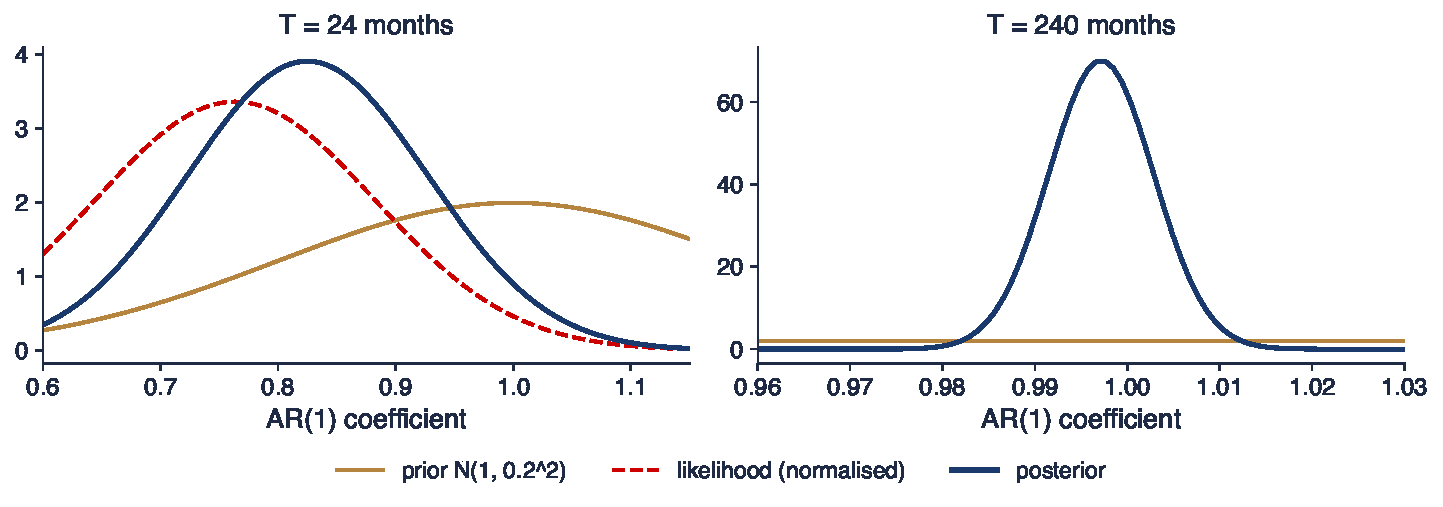
\includegraphics[width=0.97\textwidth,height=0.5\textheight,keepaspectratio]{ats_ch5_conjugate.pdf}
\end{center}
\vspace{-0.25cm}
\begin{itemize}
    \item US unemployment rate, monthly, windows ending December 2019; prior $N(1, 0.2^2)$ (random walk), $\sigma^2$ at its OLS estimate
\end{itemize}
\quantlet{ATS\_ch5\_bayes}{\qlurl{ATS_ch5_bayes}}
\end{frame}

\begin{frame}{Interpreting the update}
\itemsize{\small}
\begin{itemize}
    \item $T = 24$: OLS 0.763 (SE 0.119), posterior mean 0.825 (sd 0.102); the prior has weight 26.0\%
    \item $T = 240$: OLS 0.997, posterior 0.997; the prior weight falls to 0.1\%
    \item In a VAR, each equation has hundreds of coefficients but the same $T$: the prior keeps the weight it has at $T = 24$ here
\end{itemize}
\end{frame}

\begin{frame}{Marginal likelihood and Bayes factors}
\itemsize{\small}
\begin{itemize}
    \item $p(y\mid M) = \int p(y\mid\theta, M)p(\theta\mid M)\,d\theta$: the density of the data \emph{before} seeing them
    \begin{itemize}
        \item $M$: a model, i.e.\ a likelihood together with its prior; the integral averages the likelihood over the prior
        \item prediction-error decomposition: $\ln p(y) = \sum_t \ln p(y_t\mid y_{1:t-1})$, a sum of one-step log scores (\atschlink{https://danpele.github.io/Advanced-Time-Series/EN/Courses/chapter1_forecast_evaluation.pdf}{Chapter 1}); $y_{1:t-1}$: the data up to $t - 1$
        \item it penalises complexity automatically: a diffuse prior spreads probability over data that never occur
    \end{itemize}
    \item Bayes factor $B_{12} = p(y\mid M_1)/p(y\mid M_2)$; $2\ln B_{12} > 6$ is ``strong'' evidence \refKR
    \begin{itemize}
        \item sensitive to the prior: with an improper prior it is not defined
    \end{itemize}
    \item Hierarchical use: treat the hyperparameters $\gamma$ of the prior as parameters and maximise $p(y\mid\gamma)$ (empirical Bayes) or put a hyperprior on them \refGLP
\end{itemize}
\end{frame}

\begin{frame}{Gibbs sampling (1/2)}
\itemsize{\small}
\begin{itemize}
    \item When the joint posterior has no closed form but each \textbf{full conditional} does: draw $\theta_1\mid\theta_2, y$, then $\theta_2\mid\theta_1, y$, and repeat \refGG, \refGS
    \begin{itemize}
        \item $\theta_1$, $\theta_2$: two blocks of parameters; full conditional: the distribution of one block given the other and the data
        \item the draws form a Markov chain whose stationary distribution is the posterior
        \item discard a burn-in, then average functions of the draws (ergodic theorem)
    \end{itemize}
    \item In VARs: stochastic volatility, non-conjugate priors and set-identified SVARs (\atschlink{https://danpele.github.io/Advanced-Time-Series/EN/Courses/chapter3_structural_var_local_projections.pdf}{Chapter 3}) need Gibbs or Metropolis--Hastings steps
\end{itemize}
\end{frame}

\begin{frame}{Gibbs sampling (2/2): the linear regression}
\itemsize{\small}
\begin{itemize}
    \item Regression $y = X\beta + e$ with independent priors $\beta \sim N(b_0, V_0)$, $\sigma^2 \sim IG(a_0, d_0)$
    \begin{itemize}
        \item $b_0$, $V_0$: prior mean and covariance of $\beta$; $IG(a_0, d_0)$: inverse gamma with shape $a_0$ and scale $d_0$
    \end{itemize}
    \item Step 1, the coefficients given the variance: $\beta\mid\sigma^2, y \sim N(\bar b, \bar V)$
    \begin{itemize}
        \item $\bar V = (V_0^{-1} + X'X/\sigma^2)^{-1}$, $\bar b = \bar V(V_0^{-1}b_0 + X'y/\sigma^2)$: the Normal update of the previous slides
    \end{itemize}
    \item Step 2, the variance given the coefficients: $\sigma^2\mid\beta, y \sim IG(a_0 + T/2,\ d_0 + e'e/2)$
    \begin{itemize}
        \item $e = y - X\beta$: the residuals at the current draw of $\beta$; the data add $T/2$ to the shape and half the residual sum of squares to the scale
    \end{itemize}
\end{itemize}
\end{frame}

\begin{frame}{MCMC diagnostics}
\itemsize{\small}
\begin{itemize}
    \item \textbf{Effective sample size}: $\mathrm{ESS} = M/(1 + 2\sum_{k\ge1}\rho_k)$: the number of independent draws with the same precision
    \begin{itemize}
        \item $M$: the number of draws kept; $\rho_k$: the autocorrelation of the draws at lag $k$
        \item AR(1)-type chain: $\mathrm{ESS} = M(1 - \rho)/(1 + \rho)$; $\rho = 0.9$ keeps about 5\% of the draws
    \end{itemize}
    \item \textbf{$\widehat R$} \refGR: several chains from dispersed starts; $\widehat R = \sqrt{\hat V/W}$, $\hat V = \frac{n-1}{n}W + B/n$
    \begin{itemize}
        \item $n$: draws per chain; $W$: within-chain variance; $B$: $n\times$ the variance of the chain means; $\hat V$: the pooled variance estimate
        \item $\widehat R \approx 1$: the chains agree; current practice: rank-normalised split-$\widehat R < 1.01$ \refVGS
    \end{itemize}
    \item \textbf{Geweke} $z$: compares the mean of the first 10\% and of the last 50\% of a chain, with spectral variances; $|z| > 2$ signals non-convergence
    \item None of them proves convergence; each can reveal a failure
\end{itemize}
\end{frame}

\begin{frame}{Gibbs sampling: a bad and a good parametrisation}
\itemsize{\footnotesize}
\begin{center}
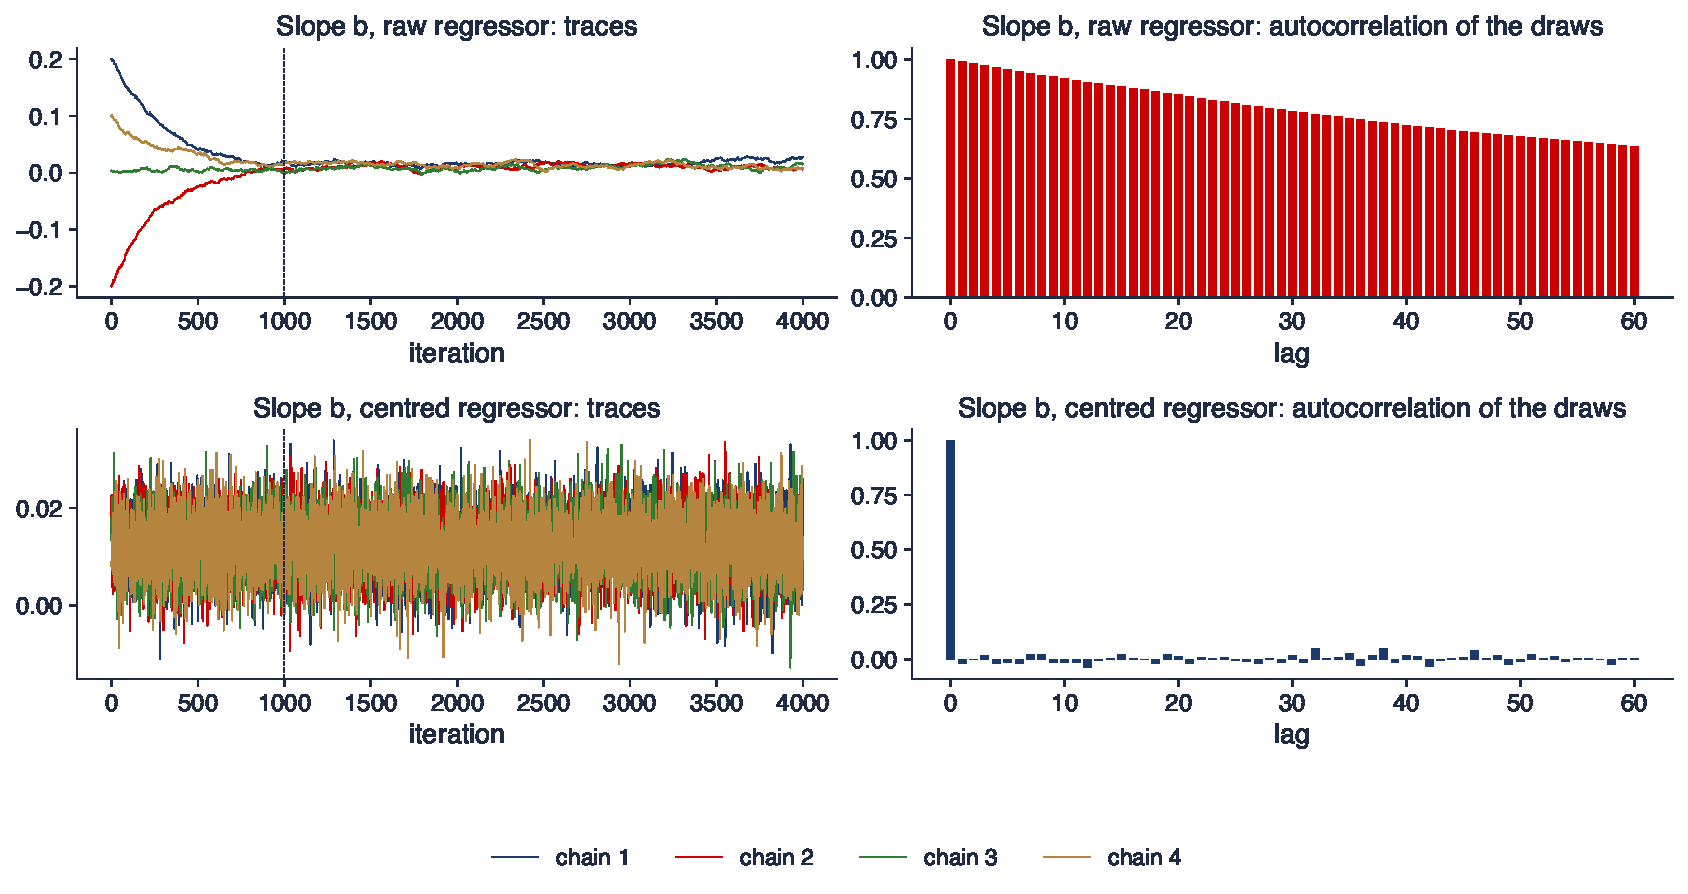
\includegraphics[width=0.97\textwidth,height=0.56\textheight,keepaspectratio]{ats_ch5_gibbs.pdf}
\end{center}
\vspace{-0.25cm}
\begin{itemize}
    \item Monthly US IP growth on lagged capacity utilisation (mean 79.0\%, sd 4.7), 1967--2019, $T = 635$; one-at-a-time Gibbs, four chains, 4\,000 draws, burn-in 1\,000
\end{itemize}
\quantlet{ATS\_ch5\_bayes}{\qlurl{ATS_ch5_bayes}}
\end{frame}

\begin{frame}{Interpreting the two samplers}
\itemsize{\small}
\begin{itemize}
    \item Raw regressor: the posterior correlation of intercept and slope is \ensuremath{-}0.998, so each conditional step moves very little
    \begin{itemize}
        \item lag-1 autocorrelation 0.992; ESS = 53 out of 12\,000 draws; $\widehat R$ = 1.32; Geweke $z$ = \ensuremath{-}2.27
    \end{itemize}
    \item Centred regressor: correlation \ensuremath{-}0.001, ESS = 11\,529, $\widehat R$ = 1.00, Geweke $z$ = 0.01
    \begin{itemize}
        \item same model, same posterior of the slope (mean 0.0123); only the sampler changed
    \end{itemize}
    \item Lesson: reparametrise or draw correlated blocks jointly; conjugate BVARs avoid the problem by drawing $B$ in one block
\end{itemize}
\end{frame}

\begin{frame}{Recap: Bayesian inference}
\itemsize{\small}
\begin{itemize}
    \item Posterior precision = prior precision + data precision; the mean is a weighted average
    \item The marginal likelihood scores a model with its prior and can choose hyperparameters
    \item Gibbs sampling needs full conditionals; check ESS, $\widehat R$ and Geweke before trusting the draws
\end{itemize}
\end{frame}


%=============================================================================
\section{The Minnesota prior and its conjugate form}
%=============================================================================

\begin{frame}{The Minnesota prior}
\itemsize{\small}
\begin{itemize}
    \item VAR($p$): $y_t = c + A_1y_{t-1} + \dots + A_py_{t-p} + u_t$; $(A_l)_{ij}$: the effect of variable $j$ at lag $l$ on variable $i$
    \begin{itemize}
        \item prior means \refLit: $\E[(A_1)_{ii}] = \delta_i$, all other coefficients 0; $\delta_i = 1$ (random walk) for persistent series, 0 (white noise) otherwise
        \item prior variances \refBGR, eq.~(2): $\Var[(A_l)_{ij}] = \lambda^2/l^2$ if $j = i$, $\vartheta\lambda^2\sigma_i^2/(l^2\sigma_j^2)$ if $j \ne i$
    \end{itemize}
    \item Hyperparameters: $\lambda$ overall tightness, $1/l^2$ lag decay, $\vartheta \in (0, 1]$ cross-variable shrinkage
    \begin{itemize}
        \item $\sigma_i^2$: residual variance of a univariate AR for $y_i$, so that $\sigma_i^2/\sigma_j^2$ fixes units
        \item $\lambda = 0$: posterior = prior; $\lambda \to \infty$: posterior mean = OLS
    \end{itemize}
    \item Original version: $\Sigma$ diagonal and fixed, each equation a separate ridge-type regression with a diffuse constant
\end{itemize}
\end{frame}

\begin{frame}{The natural conjugate prior (1/2)}
\itemsize{\small}
\begin{itemize}
    \item The VAR as a multivariate regression $Y = XB + U$, rows of $U$ i.i.d.\ $N(0, \Sigma)$
    \begin{itemize}
        \item $Y$ ($T\times n$): the observations; $X$ ($T\times k$): constant and $p$ lags; $B$ ($k\times n$): the coefficients, one column per equation
    \end{itemize}
    \item Prior \refKK: $\mathrm{vec}(B)\mid\Sigma \sim N(\mathrm{vec}(B_0), \Sigma\otimes\Omega_0)$, $\Sigma \sim IW(\Psi, d)$
    \begin{itemize}
        \item $\mathrm{vec}$: stacks the columns; $\otimes$: Kronecker product; $B_0$: prior mean; $\Omega_0$ ($k\times k$): prior covariance across regressors
        \item $IW(\Psi, d)$: inverse Wishart with scale matrix $\Psi$ and $d$ degrees of freedom
    \end{itemize}
    \item Posterior: the same families, with updated parameters
    \begin{itemize}
        \item $\bar\Omega^{-1} = \Omega_0^{-1} + X'X$, $\bar B = \bar\Omega(\Omega_0^{-1}B_0 + X'Y)$: the precision-weighted average again
        \item $\Sigma\mid Y \sim IW(\bar\Psi, T + d)$, $\bar\Psi = \Psi + \hat U'\hat U + (\bar B - B_0)'\Omega_0^{-1}(\bar B - B_0)$, $\hat U = Y - X\bar B$
    \end{itemize}
\end{itemize}
\end{frame}

\begin{frame}{The natural conjugate prior (2/2)}
\itemsize{\small}
\begin{itemize}
    \item Price of conjugacy: the Kronecker structure gives every equation the same $\Omega_0$, so $\vartheta = 1$
    \begin{itemize}
        \item Minnesota moments with $\Omega_0 = \mathrm{diag}(\lambda^2/(l^2\sigma_j^2))$ and $\E\Sigma = \mathrm{diag}(\sigma_i^2)$ ($d = n + 2$, $\Psi = \mathrm{diag}(\sigma_i^2)$)
    \end{itemize}
    \item Gain: one $k\times k$ inversion for all equations; exact draws without MCMC; a closed-form marginal likelihood (\atsapplink{atsapp1}{atssrc1}{appendix})
\end{itemize}
\end{frame}

\begin{frame}{Dummy observations}
\itemsize{\small}
\begin{itemize}
    \item Theil mixed estimation: add $T_d$ artificial rows $(Y_d, X_d)$ and run OLS on $\binom{Y_d}{Y}$, $\binom{X_d}{X}$; each row states a prior belief as if it were data
    \begin{itemize}
        \item equivalent to the NIW prior with $B_0 = (X_d'X_d)^{-1}X_d'Y_d$, $\Omega_0 = (X_d'X_d)^{-1}$ \refBGR, eq.~(5)
        \item Minnesota block: $Y_d = \mathrm{diag}(\delta_i\sigma_i)/\lambda$, $X_d = J_p\otimes\mathrm{diag}(\sigma_i)/\lambda$, $J_p = \mathrm{diag}(1, \dots, p)$
    \end{itemize}
    \item \textbf{Sum of coefficients} \refDLS: $Y_d = \mathrm{diag}(\bar y_i)/\mu$, $X_d = (\mathbf{1}_p'\otimes\mathrm{diag}(\bar y_i)/\mu,\ 0)$
    \begin{itemize}
        \item $\bar y_i$: the mean of the first $p$ observations of $y_i$; $\mathbf{1}_p$: a vector of $p$ ones; $\mu > 0$: the tightness of this prior
        \item shrinks $\Pi = I - \sum_l A_l$ to 0 (``inexact differencing''): $\mu \to 0$ gives a VAR in differences without cointegration
    \end{itemize}
    \item \textbf{Dummy initial observation} \refSims, \refSZ: one row $y = \bar y'/\phi$, $x = (\bar y'/\phi, \dots, \bar y'/\phi, 1/\phi)$
    \begin{itemize}
        \item $\bar y$: the vector of the $\bar y_i$; $\phi > 0$: its tightness; it pushes towards unit roots \emph{or} towards a stationary model whose mean is $\bar y$: allows cointegration (\atschlink{https://danpele.github.io/Advanced-Time-Series/EN/Courses/chapter4_cointegration_vecm_ardl_panel.pdf}{Chapter 4})
    \end{itemize}
\end{itemize}
\end{frame}

\begin{frame}{How much shrinkage? In-sample fit against out-of-sample accuracy}
\itemsize{\footnotesize}
\begin{center}
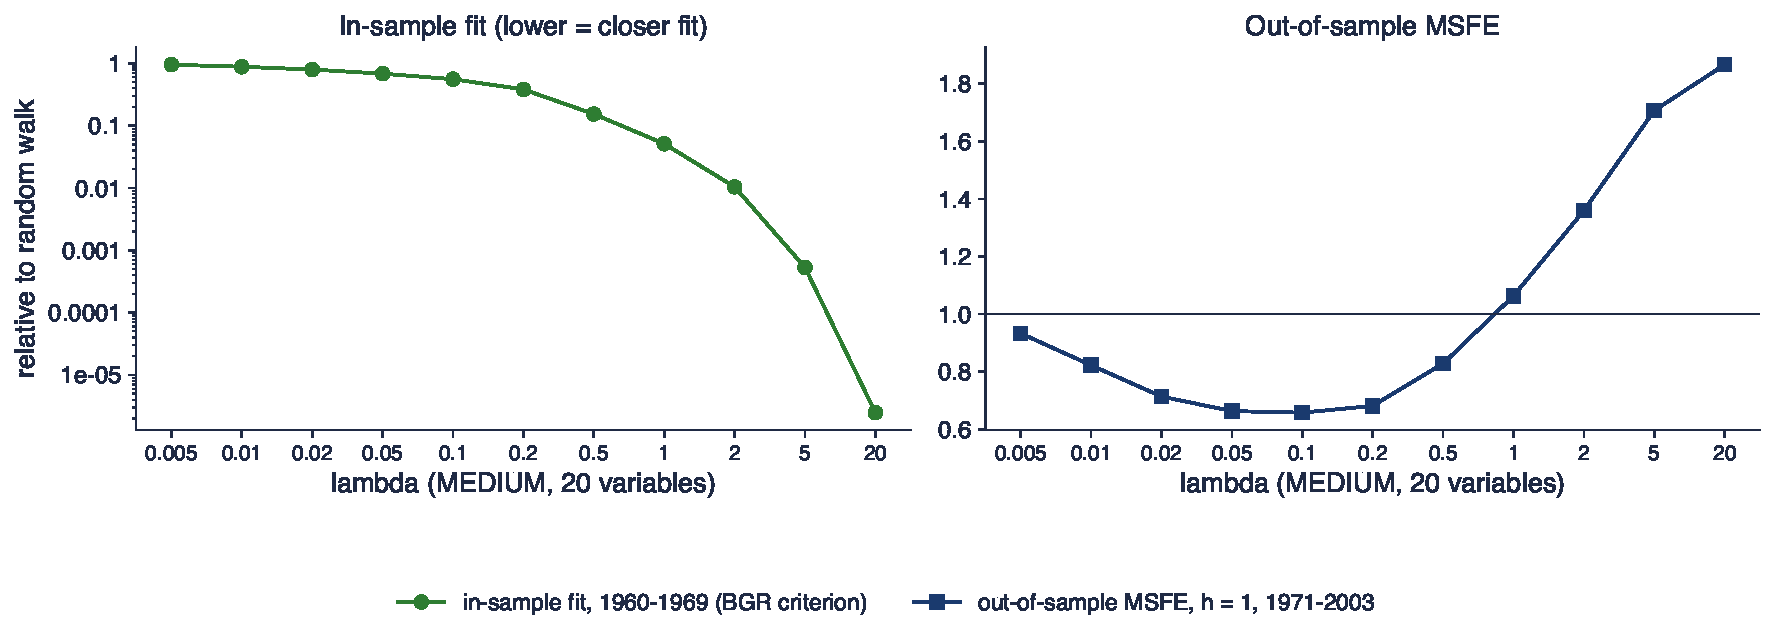
\includegraphics[width=0.97\textwidth,height=0.5\textheight,keepaspectratio]{ats_ch5_tradeoff.pdf}
\end{center}
\vspace{-0.25cm}
\begin{itemize}
    \item MEDIUM system (20 variables, $p = 13$, $k = 261$), BGR prior, rolling 10-year windows; out-of-sample: one-step MSFE of employment, CPI and the funds rate, 1971--2003, relative to a random walk
\end{itemize}
\quantlet{ATS\_ch5\_large\_bvar}{\qlurl{ATS_ch5_large_bvar}}
\end{frame}

\begin{frame}{Interpreting the trade-off}
\itemsize{\small}
\begin{itemize}
    \item The in-sample fit improves without limit as $\lambda$ grows: with $k = 261$ and $T = 120$, a loose prior interpolates the data
    \item Out of sample: U-shape; minimum 0.66 at $\lambda = 0.10$; 0.93 with $\lambda = 0.005$ (almost the random walk); 1.87 with $\lambda = 20$
    \item The shrinkage must be chosen without looking at the evaluation sample: by a fit rule (BGR) or by the marginal likelihood (GLP)
\end{itemize}
\end{frame}

\begin{frame}{Recap: Minnesota and NIW priors}
\itemsize{\small}
\begin{itemize}
    \item Minnesota: centre each equation on a random walk or white noise; shrink distant lags and other variables more
    \item The natural conjugate form keeps closed forms at the cost of $\vartheta = 1$
    \item Dummy observations implement the prior by OLS and add sum-of-coefficients and initial-observation beliefs
\end{itemize}
\end{frame}


%=============================================================================
\section{Choosing the shrinkage: hierarchical priors}
%=============================================================================

\begin{frame}{Giannone, Lenza and Primiceri (2015)}
\itemsize{\small}
\begin{itemize}
    \item Treat $\gamma = (\lambda, \mu, \phi)$ as parameters with hyperpriors: $p(\gamma\mid y) \propto p(y\mid\gamma)p(\gamma)$ \refGLP
    \begin{itemize}
        \item $p(y\mid\gamma)$ is known in closed form for the NIW prior with dummies: data plus dummies, minus dummies alone
        \item hyperpriors: Gamma with mode 0.2 and sd 0.4 for $\lambda$, mode 1 and sd 1 for $\mu$ and $\phi$
    \end{itemize}
    \item Interpretation: the marginal likelihood is an out-of-sample score of one-step predictive densities (previous section)
    \begin{itemize}
        \item so it trades fit against complexity without an evaluation sample
    \end{itemize}
    \item Use the posterior mode of $\gamma$ (as here) or integrate $\gamma$ out by Metropolis--Hastings; GLP find both forecast about as well as factor models
\end{itemize}
\end{frame}

\begin{frame}{The marginal likelihood as a function of the tightness}
\itemsize{\footnotesize}
\begin{center}
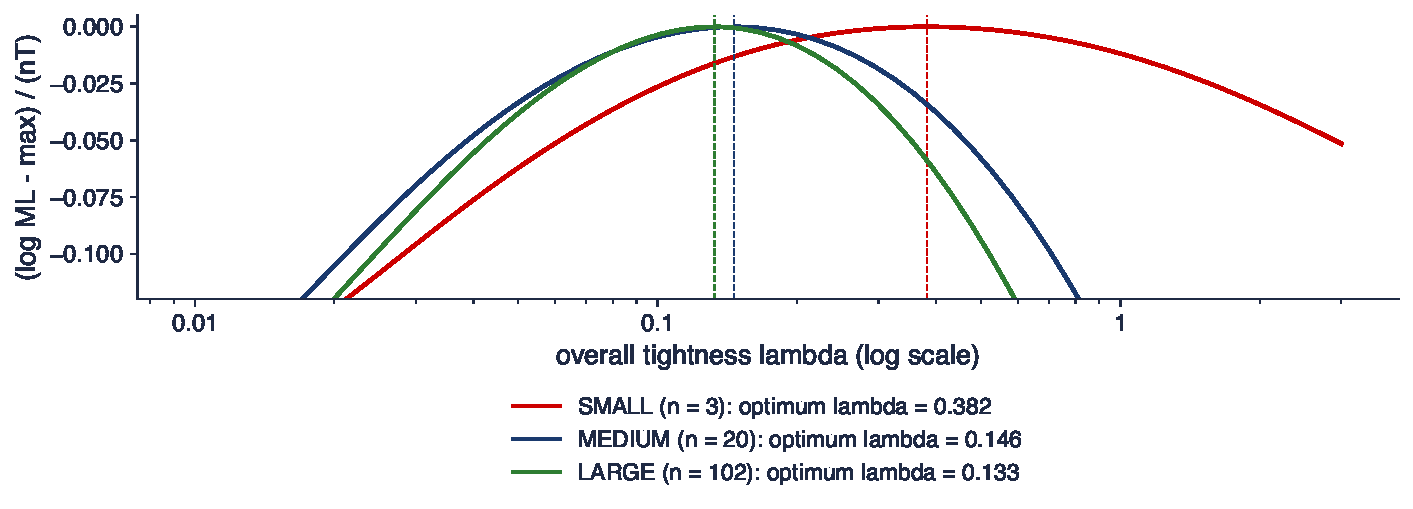
\includegraphics[width=0.97\textwidth,height=0.5\textheight,keepaspectratio]{ats_ch5_lambda.pdf}
\end{center}
\vspace{-0.25cm}
\begin{itemize}
    \item SMALL ($n = 3$), MEDIUM ($n = 20$), LARGE ($n = 102$), $p = 13$, 1960:1--2019:12 ($T = 707$); $\mu = \phi = 1$; log ML minus its maximum, divided by $nT$
\end{itemize}
\quantlet{ATS\_ch5\_large\_bvar}{\qlurl{ATS_ch5_large_bvar}}
\end{frame}

\begin{frame}{Interpreting the marginal likelihood}
\itemsize{\small}
\begin{itemize}
    \item Optimal tightness: 0.382 (SMALL), 0.146 (MEDIUM), 0.133 (LARGE): bigger systems need a tighter prior
    \item Using the textbook value $\lambda = 0.2$ costs \ensuremath{-}46.9 log points for MEDIUM and \ensuremath{-}597.2 for LARGE; $\lambda = 1$ costs \ensuremath{-}15571.6 for LARGE
    \item Joint mode with the hyperpriors: SMALL $\mu = 0.20$, $\phi = 0.44$; MEDIUM $\mu = 0.13$, $\phi = 0.44$: the data ask for tight sum-of-coefficients and initial-observation priors
\end{itemize}
\end{frame}

\begin{frame}{Two rules for one hyperparameter}
\itemsize{\small}
\begin{itemize}
    \item \textbf{BGR fit rule}: choose $\lambda$ so that the in-sample one-step fit of the key variables equals that of a small OLS VAR \refBGR, Section~3
    \begin{itemize}
        \item $\mathrm{Fit}(\lambda) = \frac13\sum_{i\in I}\mathrm{msfe}_i^{(\lambda)}/\mathrm{msfe}_i^{(0)}$ on 1960--1969; here the target is 0.43
        \item $I$: the three key variables; $\mathrm{msfe}_i^{(\lambda)}$: in-sample one-step mean squared error of variable $i$ with tightness $\lambda$; $\lambda = 0$: the prior mean alone
        \item our values: MEDIUM 0.158, LARGE 0.059 (BGR Table~1: 0.108 and 0.035 on their data set)
    \end{itemize}
    \item \textbf{GLP marginal likelihood}: re-estimated on each window; on 10-year windows the median mode is 0.34 (SMALL) and 0.28 (MEDIUM)
    \begin{itemize}
        \item 10\%--90\% range of the MEDIUM mode across windows: [0.23, 0.33]
    \end{itemize}
    \item The Python package \texttt{bvar} of the Bank of England implements the GLP optimisation for the conjugate model; the notebook compares it with our \texttt{numpy} code
\end{itemize}
\end{frame}

\begin{frame}{Recap: Hierarchical priors}
\itemsize{\small}
\begin{itemize}
    \item The marginal likelihood chooses the shrinkage; it falls as the system grows
    \item Sum-of-coefficients and initial-observation priors are chosen in the same way
    \item A fit rule is a transparent alternative when the evaluation must mimic a published study
\end{itemize}
\end{frame}


%=============================================================================
\section{Case study: large Bayesian VARs}
%=============================================================================

\begin{frame}{Bańbura, Giannone and Reichlin (2010): the design}
\itemsize{\small}
\begin{itemize}
    \item \refBGR: can a VAR with 131 variables forecast and identify shocks? Systems SMALL (employment, CPI, funds rate), MEDIUM (20), LARGE (all)
    \begin{itemize}
        \item $p = 13$; rolling 10-year windows; posterior-mean point forecasts iterated to $h = 12$; benchmark: random walk with drift
        \item Minnesota NIW prior plus sum-of-coefficients with $\tau = 10\lambda$ (Section~3.3); $\lambda$ by the fit rule on 1960--1969
    \end{itemize}
    \item Our data: FRED-MD-format panel; LARGE = the 102 series observed over 1960--2026 (aggregates and components)
    \begin{itemize}
        \item MEDIUM: the BGR list, with the S\&P 500, the effective exchange rate and nonborrowed reserves replaced by the Baa yield, the 3-month bill rate and building permits (not available for 1960--2026 or negative after 2008)
    \end{itemize}
    \item Evaluation: targets 1971--2003 (the paper), 2004--2019 and 2004--2026 (extensions); 678 forecast origins; GLP SMALL and MEDIUM added
\end{itemize}
\end{frame}

\begin{frame}{Forecast accuracy, 1971--2003}
\itemsize{\footnotesize}
\begin{center}
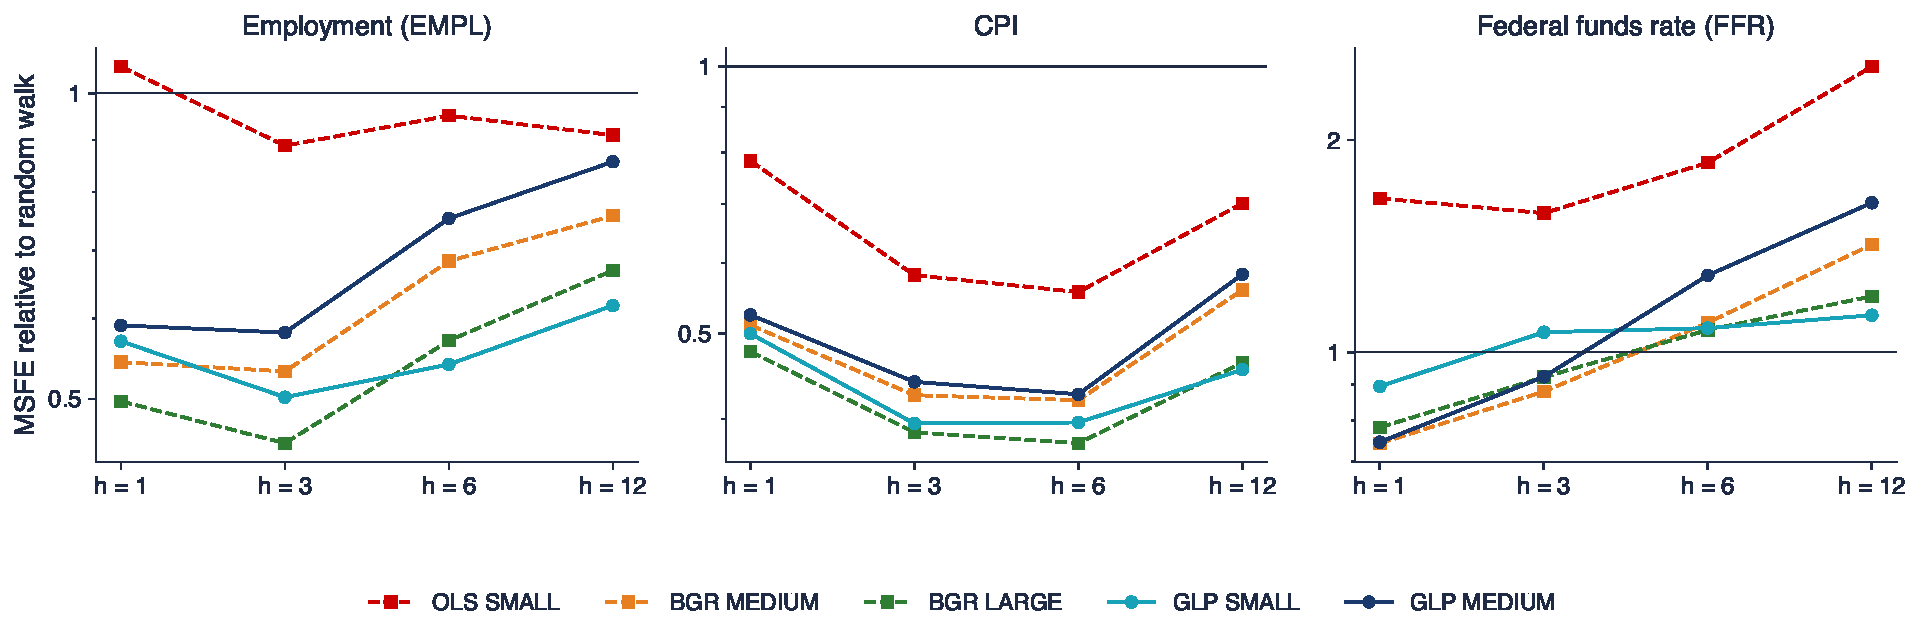
\includegraphics[width=0.97\textwidth,height=0.5\textheight,keepaspectratio]{ats_ch5_bgr.pdf}
\end{center}
\vspace{-0.25cm}
\begin{itemize}
    \item MSFE relative to the random walk with drift (log scale; below 1 = better), employment and CPI in 100 $\times$ log levels, funds rate in percent
\end{itemize}
\quantlet{ATS\_ch5\_large\_bvar}{\qlurl{ATS_ch5_large_bvar}}
\end{frame}

\begin{frame}{Interpreting the forecast comparison}
\itemsize{\small}
\begin{itemize}
    \item $h = 1$, employment: OLS SMALL 1.06, BGR MEDIUM 0.54, LARGE 0.50 (BGR Table~1: 1.14, 0.54, 0.46)
    \begin{itemize}
        \item CPI: 0.78, 0.51, 0.48; funds rate: 1.65, 0.74, 0.78
    \end{itemize}
    \item Adding variables with more shrinkage helps: LARGE beats SMALL for every variable at $h \le 6$
    \item GLP SMALL is nearly as good as the large systems for employment and CPI (0.57, 0.50): most of the gain comes from the prior, not only from the variables
    \item The funds rate beyond 3 months is hard for all models (LARGE 1.20 at $h = 12$)
\end{itemize}
\end{frame}

\begin{frame}{After 2003: the extension and March 2020}
\itemsize{\footnotesize}
\begin{center}
\scriptsize
\begin{tabular}{lcccccc}
\toprule
\textbf{Model} & \textbf{EMPL, 1} & \textbf{EMPL, 12} & \textbf{CPI, 1} & \textbf{CPI, 12} & \textbf{FFR, 1} & \textbf{FFR, 12} \\
\midrule
OLS SMALL & 0.38 & 1.08 & 1.26 & 2.43 & 0.98 & 3.51 \\
BGR MEDIUM & 0.20 & 0.66 & 0.97 & 6.49 & 0.55 & 1.91 \\
BGR LARGE & 0.19 & 0.67 & 0.92 & 3.73 & 0.45 & 1.79 \\
GLP SMALL & 0.24 & 0.33 & 0.93 & 1.07 & 0.61 & 0.67 \\
GLP MEDIUM & 0.20 & 0.28 & 0.95 & 2.55 & 0.57 & 0.91 \\
\bottomrule
\end{tabular}
\end{center}
\begin{itemize}
    \item Targets 2004:1--2019:12, relative MSFE (random walk with drift = 1)
    \item Including 2020--2026, the 12-month employment MSFE explodes: BGR MEDIUM 500.06, GLP SMALL 8.64: windows containing April 2020 fit the collapse as dynamics
    \item Remedy: scale the residual variance of the pandemic months by estimated factors \refLP, or stochastic volatility (next section)
\end{itemize}
\end{frame}

\begin{frame}{A monetary policy shock in a large VAR}
\itemsize{\small}
\begin{itemize}
    \item Recursive scheme of \refBGR, Section~4: $y_t = (X_t, r_t, Z_t)$, slow variables $X_t$ (real activity, prices), the funds rate $r_t$, fast variables $Z_t$ (money, rates, exchange rates)
    \begin{itemize}
        \item only the position of $r_t$ matters (\atschlink{https://danpele.github.io/Advanced-Time-Series/EN/Courses/chapter3_structural_var_local_projections.pdf}{Chapter 3}): no ordering inside the blocks is needed
    \end{itemize}
    \item Bayesian bands: for each draw $(B, \Sigma)$ from the NIW posterior, compute the Cholesky impact column and the responses; report posterior quantiles
    \begin{itemize}
        \item 500 draws, 100 bp shock, sample 1961--2002, $p = 13$; SMALL with a nearly flat prior
    \end{itemize}
    \item These are the posterior bands \atschlink{https://danpele.github.io/Advanced-Time-Series/EN/Courses/chapter3_structural_var_local_projections.pdf}{Chapter 3} announced: pointwise credible intervals, conditional on the identifying assumption
\end{itemize}
\end{frame}

\begin{frame}{Responses to a 100 bp funds-rate shock}
\itemsize{\footnotesize}
\begin{center}
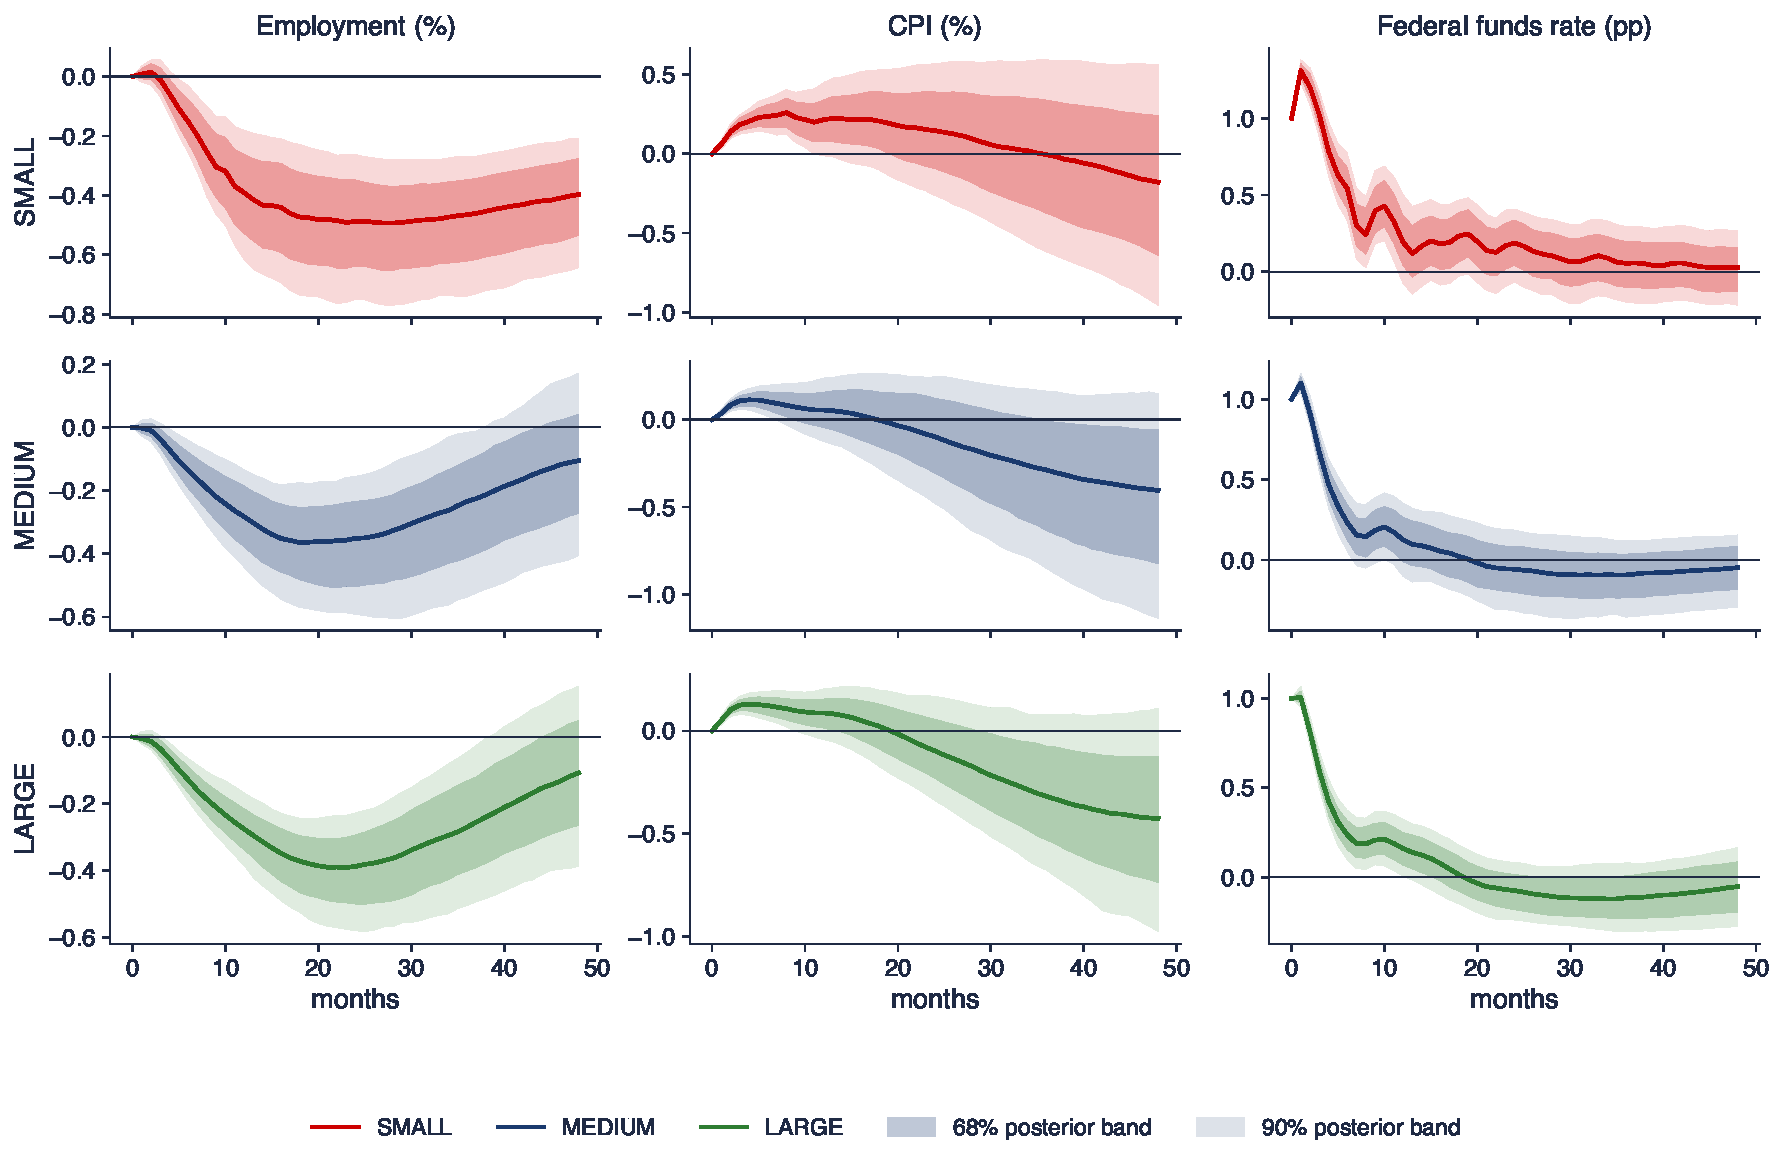
\includegraphics[width=0.97\textwidth,height=0.6\textheight,keepaspectratio]{ats_ch5_bvar_irf.pdf}
\end{center}
\vspace{-0.25cm}
\begin{itemize}
    \item Posterior medians with 68\% and 90\% bands; rows: SMALL, MEDIUM, LARGE; employment and CPI in percent
\end{itemize}
\quantlet{ATS\_ch5\_large\_bvar}{\qlurl{ATS_ch5_large_bvar}}
\end{frame}

\begin{frame}{Interpreting the responses}
\itemsize{\small}
\begin{itemize}
    \item Employment: trough \ensuremath{-}0.49\% (SMALL, month 28), \ensuremath{-}0.39\% (LARGE, month 23); after four years LARGE is back to \ensuremath{-}0.11\% (band [\ensuremath{-}0.39, 0.15])
    \item CPI: the price puzzle shrinks from 0.26\% (SMALL) to 0.13\% (LARGE); after four years LARGE gives \ensuremath{-}0.43\% (band [\ensuremath{-}0.97, 0.11])
    \item As in BGR: more information makes the employment response less persistent and the price response more plausible
    \item The bands do not widen with 102 variables: the prior pays for the extra coefficients
\end{itemize}
\end{frame}

\begin{frame}{Recap: Large BVARs}
\itemsize{\small}
\begin{itemize}
    \item With shrinkage that grows with the system, a 102-variable VAR forecasts better than a 3-variable OLS VAR
    \item The 1971--2003 results of BGR replicate on today's data; after 2020 the homoskedastic BVAR fails
    \item Large information sets reduce the price puzzle of small monetary VARs
\end{itemize}
\end{frame}


%=============================================================================
\section{Stochastic volatility in BVARs}
%=============================================================================

\begin{frame}{Large BVARs with stochastic volatility}
\itemsize{\small}
\begin{itemize}
    \item \textbf{Common volatility} \refCCMa: $u_t = \sqrt{f_t}\,\varepsilon_t$, $\varepsilon_t \sim N(0, \Sigma)$, $\ln f_t = \phi\ln f_{t-1} + \nu_t$
    \begin{itemize}
        \item $u_t$: the VAR residual; $f_t > 0$: a volatility factor common to all equations; $\phi$: its persistence; $\nu_t$: its shock
        \item given $f_{1:T}$, the model is a weighted conjugate BVAR (rows divided by $\sqrt{f_t}$); $f_t$ is drawn by a Kim--Shephard--Chib step
    \end{itemize}
    \item \textbf{Variable-specific volatilities} \refCCMb, \refClark: $\Sigma_t = A^{-1}H_tA^{-1\prime}$, $H_t$ diagonal with log-AR volatilities \refPrim
    \begin{itemize}
        \item $A$: lower triangular with unit diagonal (the contemporaneous relations); $H_t$: the time-varying variances of the orthogonalised shocks
        \item conjugacy is lost; the triangular algorithm draws the equations one at a time and makes $n = 100$ feasible
    \end{itemize}
    \item Gains: mainly in density forecasts (calibrated intervals) and in robustness to outliers such as 2020
\end{itemize}
\end{frame}

\begin{frame}{A common volatility factor in the BVAR residuals}
\itemsize{\footnotesize}
\begin{center}
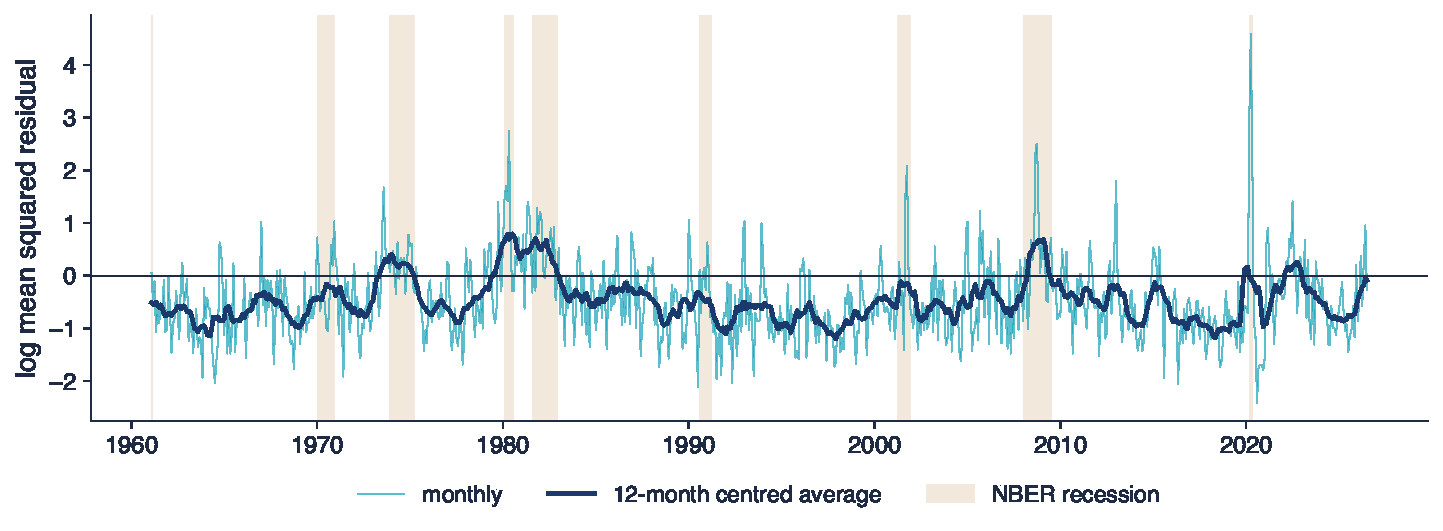
\includegraphics[width=0.97\textwidth,height=0.5\textheight,keepaspectratio]{ats_ch5_common_vol.pdf}
\end{center}
\vspace{-0.25cm}
\begin{itemize}
    \item MEDIUM BVAR (GLP hyperparameters), 1960--2026: log of the cross-sectional mean of the squared standardised residuals
\end{itemize}
\quantlet{ATS\_ch5\_large\_bvar}{\qlurl{ATS_ch5_large_bvar}}
\end{frame}

\begin{frame}{Interpreting the volatility proxy}
\itemsize{\small}
\begin{itemize}
    \item Common movements: the residual variance rises in every recession and falls in the Great Moderation (1960--1984 is 1.28 times 1985--2007)
    \item April 2020 is 176 times the median month: a homoskedastic Gaussian BVAR treats it as an ordinary observation
    \item This is the case for the common-volatility model (one extra state) before the full variable-specific model; \atschlink{https://danpele.github.io/Advanced-Time-Series/EN/Courses/chapter6_state_space_models_bayesian_filtering.pdf}{Chapter 6} gives the filtering tools
\end{itemize}
\end{frame}


%=============================================================================
\section{Approximate factor models}
%=============================================================================

\begin{frame}{The approximate factor model}
\itemsize{\small}
\begin{itemize}
    \item $x_{it} = \lambda_i'F_t + e_{it}$, $i = 1, \dots, N$, $t = 1, \dots, T$; $F_t$: $r$ common factors, $\lambda_i$: loadings, $e_{it}$: idiosyncratic
    \begin{itemize}
        \item \emph{approximate} \refCR: the $e_{it}$ may be weakly correlated across $i$ and over $t$, provided the correlation is bounded as $N \to \infty$
        \item $\Lambda$ ($N\times r$): the stacked loadings; $X$ ($T\times N$): the panel; $\Sigma_\Lambda$: a positive definite limit
        \item pervasiveness: $\Lambda'\Lambda/N \to \Sigma_\Lambda > 0$, every factor affects many series; the $r$ largest eigenvalues of $XX'$ grow with $N$, the others do not
    \end{itemize}
    \item Identification: $\Lambda F_t = (\Lambda H)(H^{-1}F_t)$ for any invertible $H$: only the factor space is identified
    \begin{itemize}
        \item normalisation for PCA: $F'F/T = I_r$ and $\Lambda'\Lambda$ diagonal
    \end{itemize}
    \item Static form of a dynamic model: lags of the dynamic factors are stacked in $F_t$ \refSWc; the generalised dynamic model works in the frequency domain \refFHLR
\end{itemize}
\end{frame}

\begin{frame}{Principal components}
\itemsize{\small}
\begin{itemize}
    \item Least squares: $\min_{F, \Lambda}\sum_{i,t}(x_{it} - \lambda_i'F_t)^2$ with $F'F/T = I$: $\hat F = \sqrt T\times$ the first $r$ eigenvectors of $XX'$, $\hat\Lambda = X'\hat F/T$
    \begin{itemize}
        \item standardise each series first: PCA is not scale invariant
    \end{itemize}
    \item Consistency \refSWa, \refBai: $\hat F_t \to HF_t$ as $N, T \to \infty$ at rate $\min(\sqrt N, \sqrt T)$
    \begin{itemize}
        \item $H$: an invertible $r\times r$ rotation; PCA recovers the factors up to this rotation
        \item if $\sqrt T/N \to 0$, the estimated factors can be used as regressors as if observed (no generated-regressor correction)
    \end{itemize}
    \item Missing values and mixed start dates: EM \refSWb, \refMN: fill with 0, run PCA, refill the missing cells with $\hat\lambda_i'\hat F_t$, iterate
\end{itemize}
\end{frame}

\begin{frame}{The FRED-MD database}
\itemsize{\small}
\begin{itemize}
    \item \refMN: about 130 US monthly series since 1959, updated monthly, with a transformation code per series and vintages for real-time work
    \begin{itemize}
        \item eight groups: output and income, labour market, housing, consumption and orders, money and credit, interest and exchange rates, prices, stock market
        \item outliers: an observation more than 10 interquartile ranges from the median is set to missing (3 cells here)
    \end{itemize}
    \item Our panel: 117 FRED-MD series that FRED distributes (stock-market series are not), 1960:1--2026:7, 4.5\% missing cells
    \begin{itemize}
        \item the official file (current.csv of the St.~Louis Fed) can replace it in the notebook with one line
    \end{itemize}
    \item Current vintage only: the results are pseudo out of sample, not real time \refCS
\end{itemize}
\end{frame}

\begin{frame}{Factors of the FRED-MD panel}
\itemsize{\footnotesize}
\begin{center}
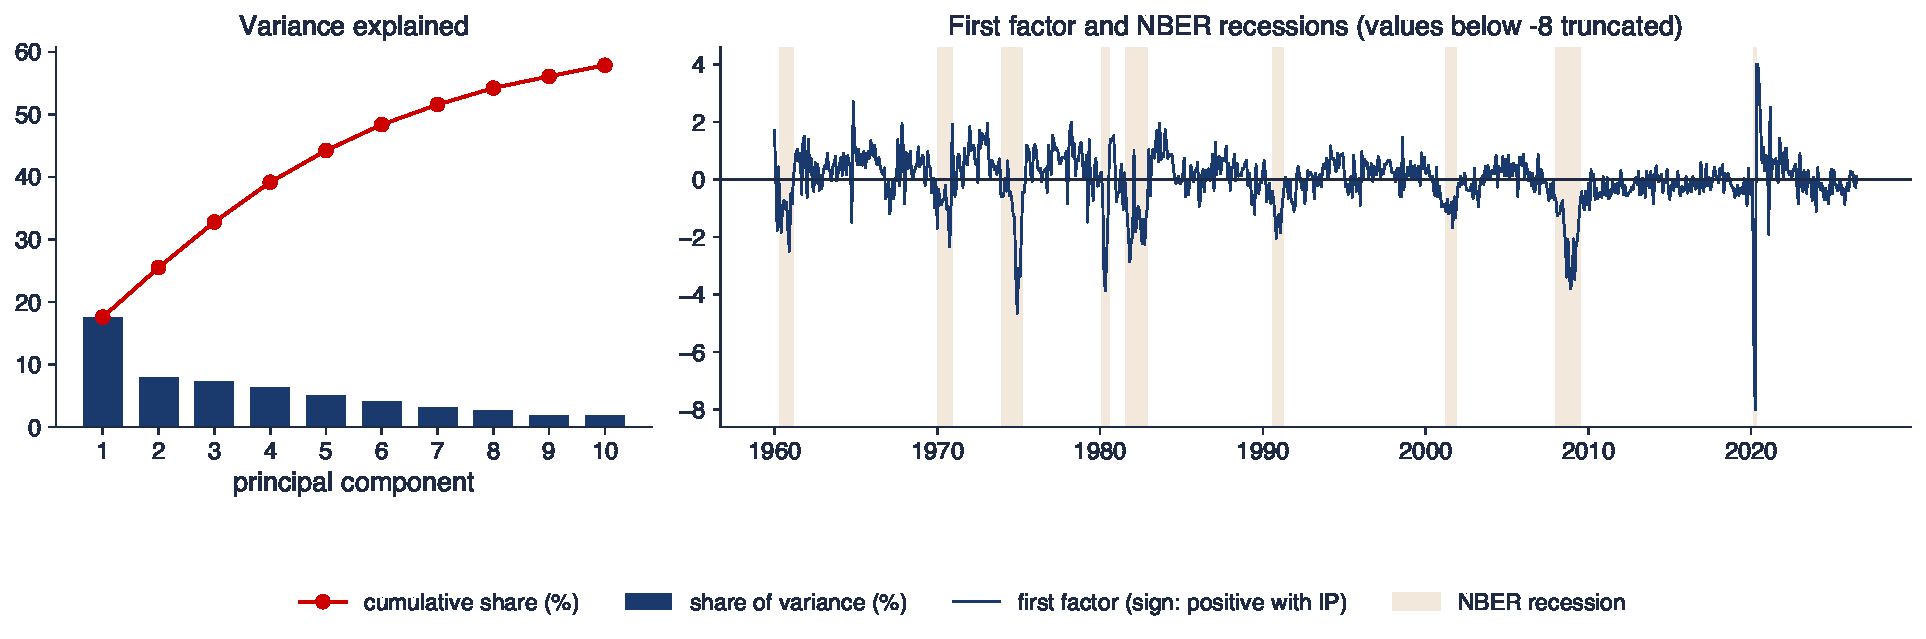
\includegraphics[width=0.97\textwidth,height=0.5\textheight,keepaspectratio]{ats_ch5_factors.pdf}
\end{center}
\vspace{-0.25cm}
\begin{itemize}
    \item Left: share of the variance of the standardised panel explained by each principal component; right: the first factor (EM, 8 factors), NBER recessions shaded
\end{itemize}
\quantlet{ATS\_ch5\_factors}{\qlurl{ATS_ch5_factors}}
\end{frame}

\begin{frame}{Interpreting the factors}
\itemsize{\small}
\begin{itemize}
    \item The first component explains 17.6\%, the second 7.9\%; five explain 44.2\%, eight 54.2\%
    \item The first factor is a real activity index: correlation \ensuremath{-}0.58 with the NBER recession indicator; its minimum is April 2020
    \item No component dominates: macro panels have a few strong factors and a long tail of weak ones, which makes the number of factors a real question
\end{itemize}
\end{frame}

\begin{frame}{How many factors? Bai and Ng (2002)}
\itemsize{\small}
\begin{itemize}
    \item $V(k) = (NT)^{-1}\sum_{i,t}(x_{it} - \hat\lambda_i'\hat F_t)^2$ after $k$ components; it falls with $k$, so it needs a penalty \refBN
    \begin{itemize}
        \item $IC_{p1}(k) = \ln V(k) + k\frac{N + T}{NT}\ln\frac{NT}{N + T}$, $IC_{p2}(k) = \ln V(k) + k\frac{N + T}{NT}\ln C_{NT}^2$, $C_{NT}^2 = \min(N, T)$
        \item $IC_{p3}(k) = \ln V(k) + k\ln C_{NT}^2/C_{NT}^2$; choose the $k$ that minimises the criterion; the penalty grows with $k$ and vanishes as $N, T \to \infty$
        \item $PC_{p}$ versions: $V(k) + k\hat\sigma^2 g(N, T)$ with $\hat\sigma^2 = V(k_{\max})$, $g(N, T)$ the same penalties: depend on $k_{\max}$, the largest $k$ tried
    \end{itemize}
    \item Our panel ($k_{\max} = 15$): $IC_{p1}$ = 8, $IC_{p2}$ = 8, $IC_{p3}$ = 10, $PC_{p1}$ = 13, $PC_{p2}$ = 11
    \begin{itemize}
        \item the criteria disagree when the eigenvalues decline slowly; report the choice and its sensitivity
    \end{itemize}
    \item For forecasting, the number of factors in the regression is chosen separately (by BIC), as in diffusion-index forecasts
\end{itemize}
\end{frame}

\begin{frame}{The economic content of the factors}
\itemsize{\footnotesize}
\begin{center}
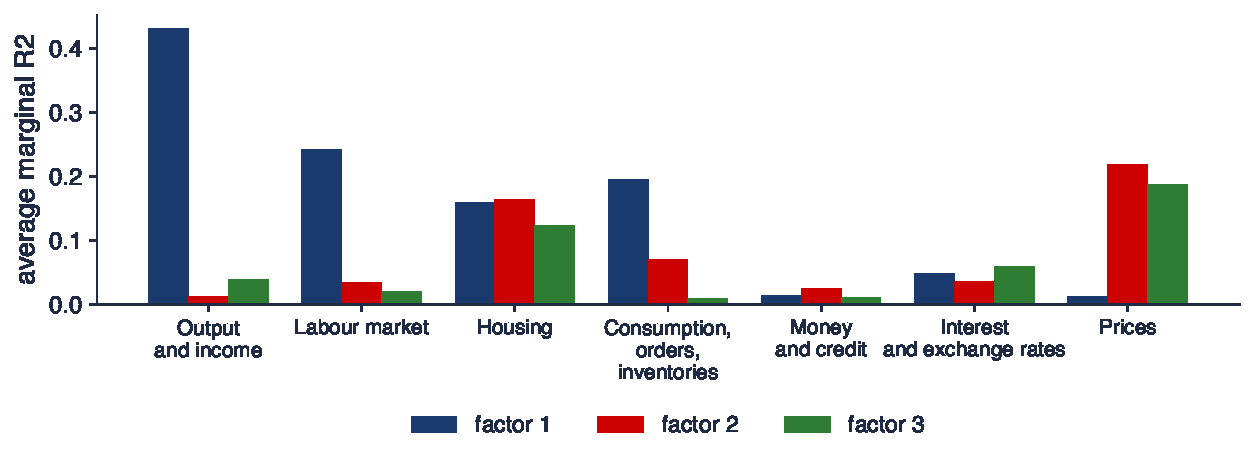
\includegraphics[width=0.97\textwidth,height=0.5\textheight,keepaspectratio]{ats_ch5_mr2.pdf}
\end{center}
\vspace{-0.25cm}
\begin{itemize}
    \item Average marginal $R^2$ of the regression of each standardised series on one factor, by group (as in McCracken and Ng 2016)
\end{itemize}
\quantlet{ATS\_ch5\_factors}{\qlurl{ATS_ch5_factors}}
\end{frame}

\begin{frame}{Interpreting the marginal R2}
\itemsize{\small}
\begin{itemize}
    \item Factor 1 is real activity: $R^2$ 0.43 for output, 0.24 for labour; the best single series has 0.78
    \item Factors 2 and 3 load on prices (0.22, 0.19) and housing (0.16, 0.12)
    \item Interest rates load weakly on the first three factors: monetary information sits in later factors or in the rates themselves, the motivation for the FAVAR
    \item Labels are a rotation choice: the factor space, not each factor, is identified
\end{itemize}
\end{frame}

\begin{frame}{Diffusion-index forecasts: Stock and Watson (2002)}
\itemsize{\small}
\begin{itemize}
    \item \refSWb: $y_{t+h}^h = \alpha_h + \beta_h'\hat F_t + \sum_{j=0}^{p}\gamma_{hj}z_{t-j} + \varepsilon_{t+h}$ (direct forecast, one equation per $h$)
    \begin{itemize}
        \item $y_{t+h}^h$: the target over the next $h$ months, annualised; $\hat F_t$: the estimated factors; $z_t$: the target's own current growth; $\alpha_h$, $\beta_h$, $\gamma_{hj}$: coefficients estimated by OLS for each $h$
        \item real series: $y_{t+h}^h = \frac{1200}{h}\ln(Y_{t+h}/Y_t)$; prices: $\frac{1200}{h}\ln(P_{t+h}/P_t) - 1200\ln(P_t/P_{t-1})$ ($Y_t$, $P_t$: levels)
        \item DI: factors only, $k \in \{1, \dots, 12\}$ by BIC; DI-AR, Lag: factors and $p \in \{0, \dots, 5\}$ lags by BIC; benchmark: AR with BIC lags
    \end{itemize}
    \item Recursive: factors re-estimated at each origin by EM on the data available then; origins from 1970:1
    \begin{itemize}
        \item evaluation 1970--1998 (the paper) and 1999--2019 (extension), by forecast origin
    \end{itemize}
    \item Targets: industrial production, payroll employment, CPI inflation; $h = 1, 6, 12$ months
\end{itemize}
\end{frame}

\begin{frame}{Diffusion-index forecasts against an AR}
\itemsize{\footnotesize}
\begin{center}
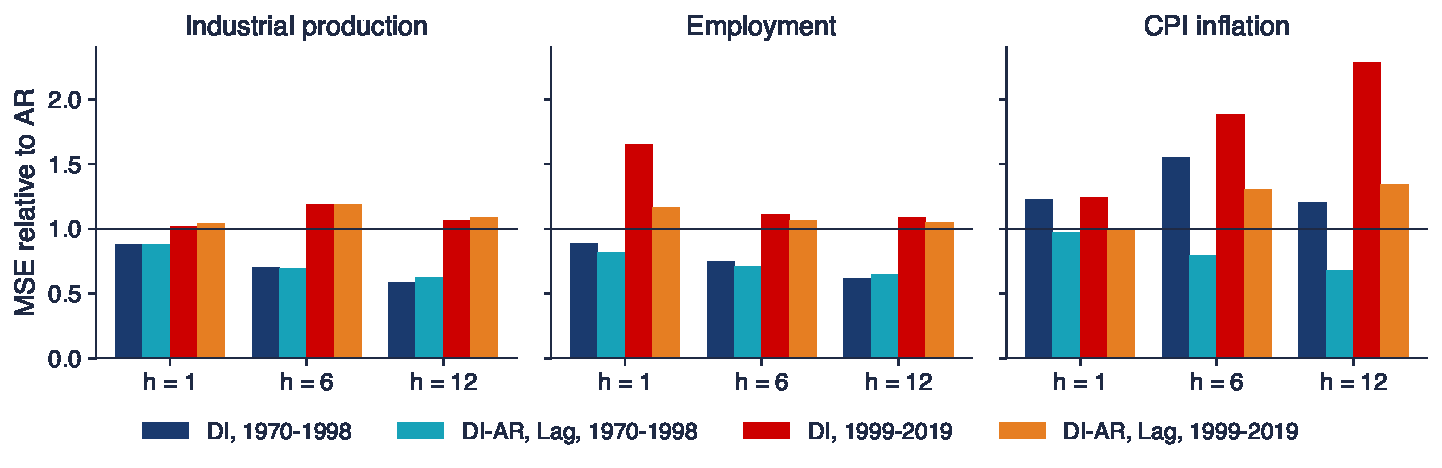
\includegraphics[width=0.97\textwidth,height=0.5\textheight,keepaspectratio]{ats_ch5_di.pdf}
\end{center}
\vspace{-0.25cm}
\begin{itemize}
    \item MSE relative to the AR forecast with BIC lags (below 1 = better)
\end{itemize}
\quantlet{ATS\_ch5\_factors}{\qlurl{ATS_ch5_factors}}
\end{frame}

\begin{frame}{Interpreting the diffusion indexes}
\itemsize{\small}
\begin{itemize}
    \item 1970--1998: large gains for real activity at $h = 12$: IP 0.58, employment 0.62; for inflation only with own lags (DI-AR, Lag 0.68)
    \item 1999--2019: the gains vanish (IP 1.07, employment 1.09, inflation 1.35): the Great Moderation made activity less predictable from the panel
    \item BIC selects a median of 7 factors (10\%--90\%: 5--12) for DI-AR, Lag at $h = 12$
    \item Bayesian shrinkage and principal components give highly correlated forecasts in large panels \refDGRa: two ways to use the same information
\end{itemize}
\end{frame}

\begin{frame}{Recap: Factor models}
\itemsize{\small}
\begin{itemize}
    \item A few factors summarise a hundred series; PCA estimates the factor space consistently as $N, T \to \infty$
    \item Bai--Ng criteria choose the number of factors; check their sensitivity
    \item Diffusion indexes helped strongly before 1999 and much less after: evaluate on more than one period
\end{itemize}
\end{frame}


%=============================================================================
\section{Factor-augmented VARs}
%=============================================================================

\begin{frame}{FAVAR: Bernanke, Boivin and Eliasz (2005)}
\itemsize{\footnotesize}
\begin{columns}[T]
\begin{column}{0.30\textwidth}
\centering
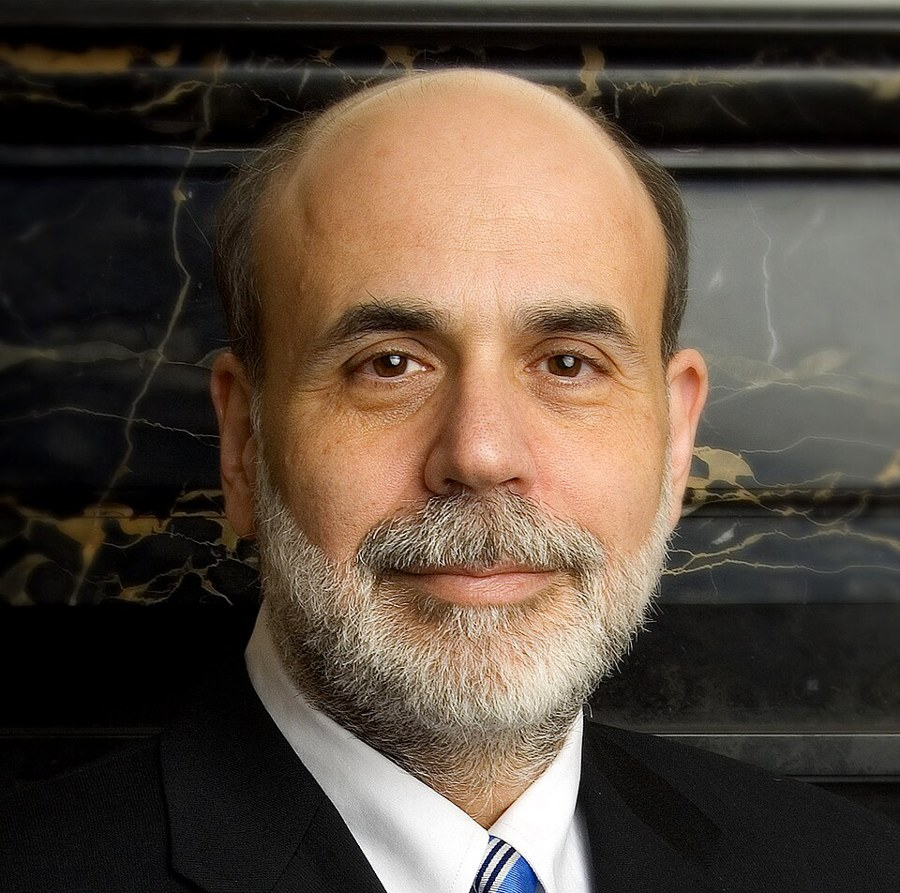
\includegraphics[height=0.32\textheight]{ch5_bernanke_2008.jpg}\\[1mm]
\imgcap{Ben Bernanke, 2008}
\imgcredit{https://commons.wikimedia.org/wiki/File:Ben_Bernanke_official_portrait_(cropped).jpg}{Photo: Federal Reserve (2008); public domain; Wikimedia Commons}
\end{column}
\begin{column}{0.68\textwidth}
\begin{itemize}
    \item \refBBE: $\binom{F_t}{Y_t} = \Phi(L)\binom{F_{t-1}}{Y_{t-1}} + v_t$, $X_t = \Lambda^fF_t + \Lambda^yY_t + e_t$, $Y_t$ = funds rate
    \begin{itemize}
        \item $F_t$: $K$ unobserved factors; $X_t$: the large panel; $\Lambda^f$, $\Lambda^y$: loadings; $\Phi(L)$: a lag polynomial; $v_t$, $e_t$: errors
        \item the VAR sees the information of 100 series through $K$ factors; responses are available for every series in $X_t$
    \end{itemize}
    \item Two-step estimation (Section III): principal components $\hat C_t$ of $X_t$; slow factors from slow-moving series; remove $Y_t$: $\hat F_t = \hat C_t - \hat b_Y Y_t$
    \begin{itemize}
        \item $K = 3$, VAR(13), 1960:1--2001:8 (ours: $T = 500$, $N = 102$ balanced series, 76 slow); Cholesky with $Y_t$ last; 25 bp shock
    \end{itemize}
    \item Prices and money enter as monthly growth rates; responses are cumulated to levels
\end{itemize}
\end{column}
\end{columns}
\end{frame}

\begin{frame}{FAVAR responses to a 25 bp monetary policy shock}
\itemsize{\footnotesize}
\begin{center}
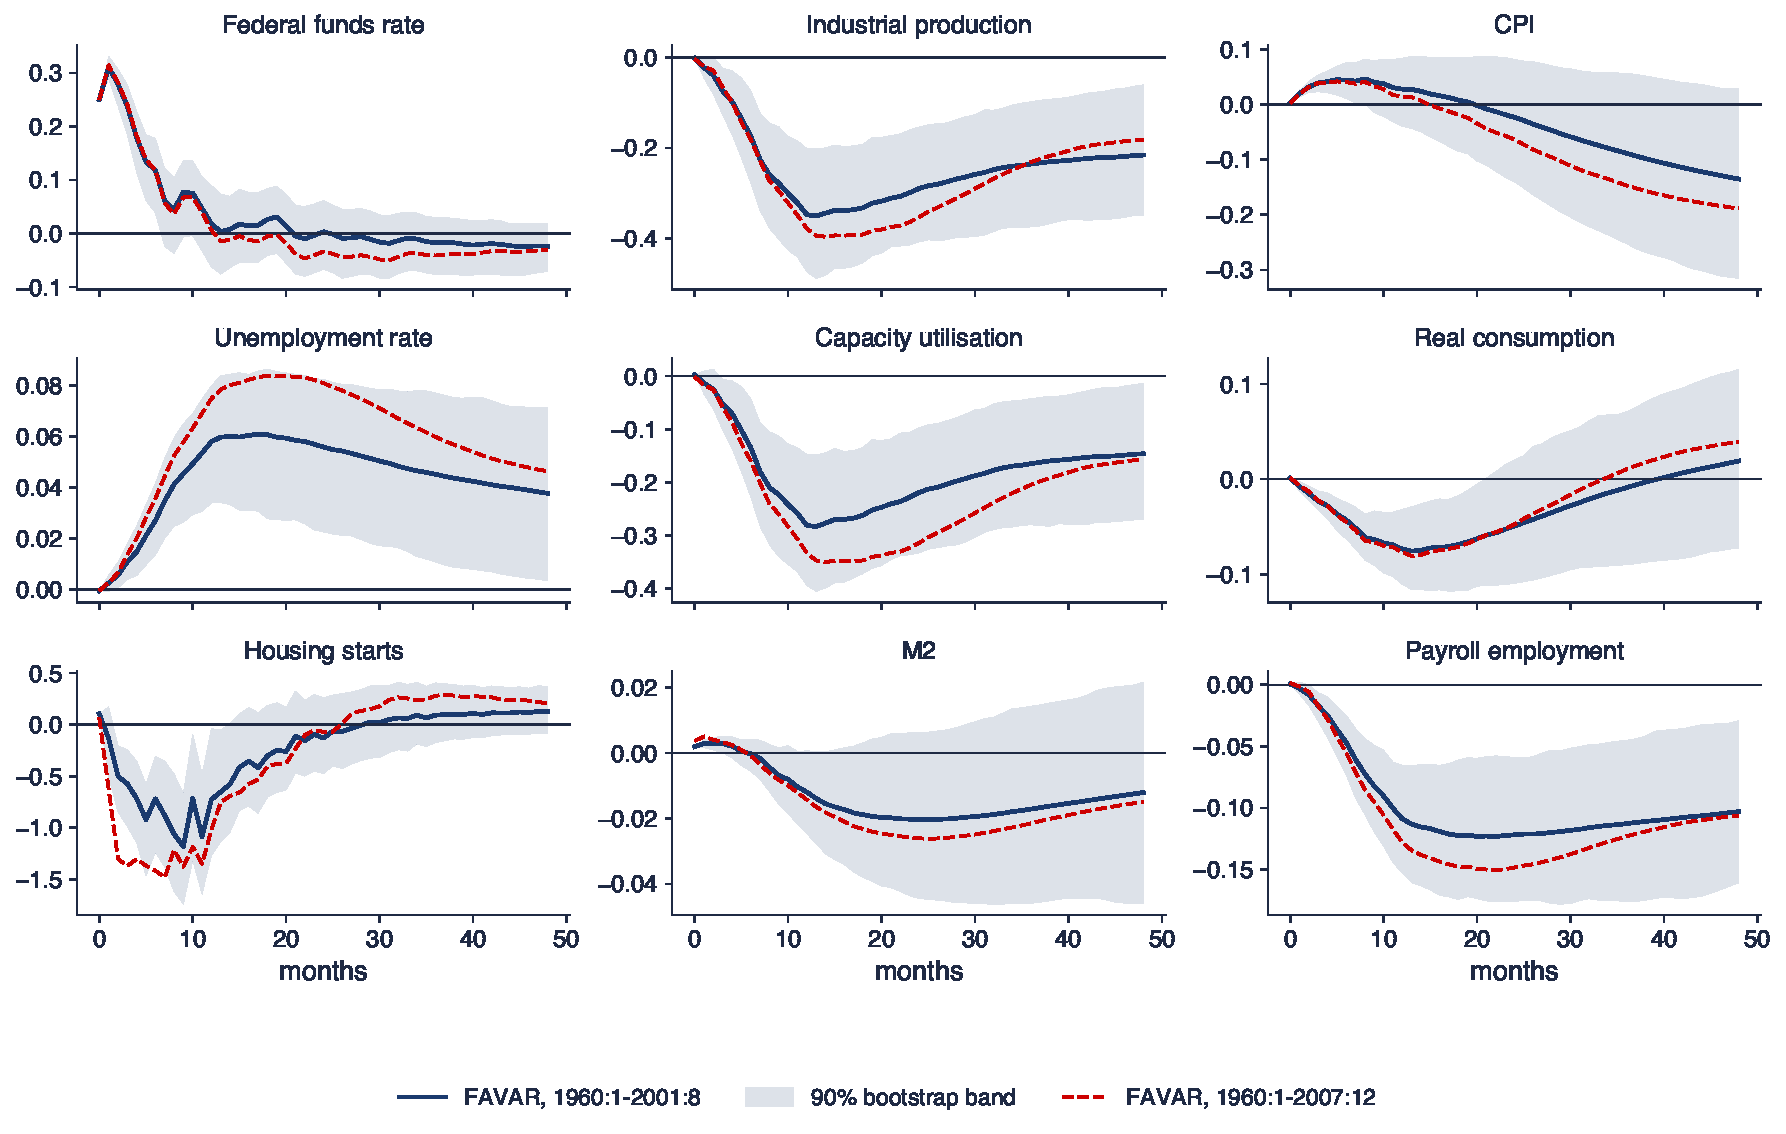
\includegraphics[width=0.97\textwidth,height=0.6\textheight,keepaspectratio]{ats_ch5_favar.pdf}
\end{center}
\vspace{-0.25cm}
\begin{itemize}
    \item Levels in percent (rates and unemployment in pp); 90\% residual-bootstrap bands, factors treated as data; dashed: sample to 2007:12
\end{itemize}
\quantlet{ATS\_ch5\_favar}{\qlurl{ATS_ch5_favar}}
\end{frame}

\begin{frame}{Interpreting the FAVAR}
\itemsize{\small}
\begin{itemize}
    \item Real activity falls with a lag: IP trough \ensuremath{-}0.35\% after 13 months, capacity utilisation \ensuremath{-}0.28 pp, payrolls \ensuremath{-}0.12\%, unemployment up by 0.061 pp
    \item Housing starts react first and most (\ensuremath{-}1.18\% after 9 months): the interest-sensitive sector
    \item The price puzzle is small (at most 0.046\%, month 8); CPI ends at \ensuremath{-}0.14\% after 48 months (band [\ensuremath{-}0.32, 0.03]); to 2007: \ensuremath{-}0.19\%
    \item Seminar 5, B4: with $K = 1$ or $K = 5$ the puzzle returns; the choice of $K$ is an identifying assumption, not a detail
\end{itemize}
\end{frame}


%=============================================================================
\section{Dynamic factor models in state-space form}
%=============================================================================

\begin{frame}{The dynamic factor model}
\itemsize{\small}
\begin{itemize}
    \item Measurement: $x_t = \Lambda f_t + e_t$, $e_t \sim N(0, \Psi)$, $\Psi$ diagonal; transition: $f_t = A_1f_{t-1} + \dots + A_qf_{t-q} + u_t$, $u_t \sim N(0, Q)$
    \begin{itemize}
        \item $x_t$: the $N$ observed series; $f_t$: the $r$ factors; $\Lambda$: loadings; $e_t$: idiosyncratic errors with diagonal covariance $\Psi$; $A_j$: factor VAR($q$) matrices; $Q$: covariance of the factor shocks $u_t$
        \item a state-space model (\atschlink{https://danpele.github.io/Time-Series-Analysis/EN/Courses/chapter10_state_space_kalman_markov_switching.pdf}{TSA, Chapter 10}; \atschlink{https://danpele.github.io/Advanced-Time-Series/EN/Courses/chapter6_state_space_models_bayesian_filtering.pdf}{Chapter 6}): state $s_t = (f_t', \dots, f_{t-m}')'$, $m \ge q - 1$ lags; Kalman filter and smoother
    \end{itemize}
    \item \textbf{Two-step} \refDGRb: PCA for $\hat f_t$, OLS for $\Lambda$ and $\Psi$, a VAR on $\hat f_t$ for $A$ and $Q$, then the Kalman smoother re-estimates $f_t$
    \begin{itemize}
        \item consistent for large $N$ and $T$ even though $\Psi$ diagonal is misspecified
    \end{itemize}
    \item \textbf{Quasi-maximum likelihood by EM} \refDGRc, \refBM: E-step = Kalman smoother, M-step = regressions on smoothed moments; handles any pattern of missing data and idiosyncratic AR(1) terms
\end{itemize}
\end{frame}

\begin{frame}{Missing data are not a problem for the Kalman filter}
\itemsize{\small}
\begin{itemize}
    \item At time $t$, keep only the observed rows: $x_t^o = W_tx_t$, $\Lambda_t = W_t\Lambda$, $\Psi_t = W_t\Psi W_t'$ with $W_t$ a selection matrix
    \begin{itemize}
        \item if nothing is observed, the update step is skipped and the prediction is carried forward
    \end{itemize}
    \item \textbf{Ragged edge}: at the end of the sample each series stops at a different month (publication lags); the filter uses whatever is there
    \begin{itemize}
        \item the same mechanism handles series that start late (services confidence from 2002) and quarterly series observed every third month
    \end{itemize}
    \item This is why nowcasting is a filtering problem, and why \atschlink{https://danpele.github.io/Advanced-Time-Series/EN/Courses/chapter6_state_space_models_bayesian_filtering.pdf}{Chapter 6} develops the filter in full
\end{itemize}
\end{frame}


%=============================================================================
\section{Mixed frequencies and nowcasting}
%=============================================================================

\begin{frame}{The nowcasting problem}
\itemsize{\footnotesize}
\begin{columns}[T]
\begin{column}{0.32\textwidth}
\centering
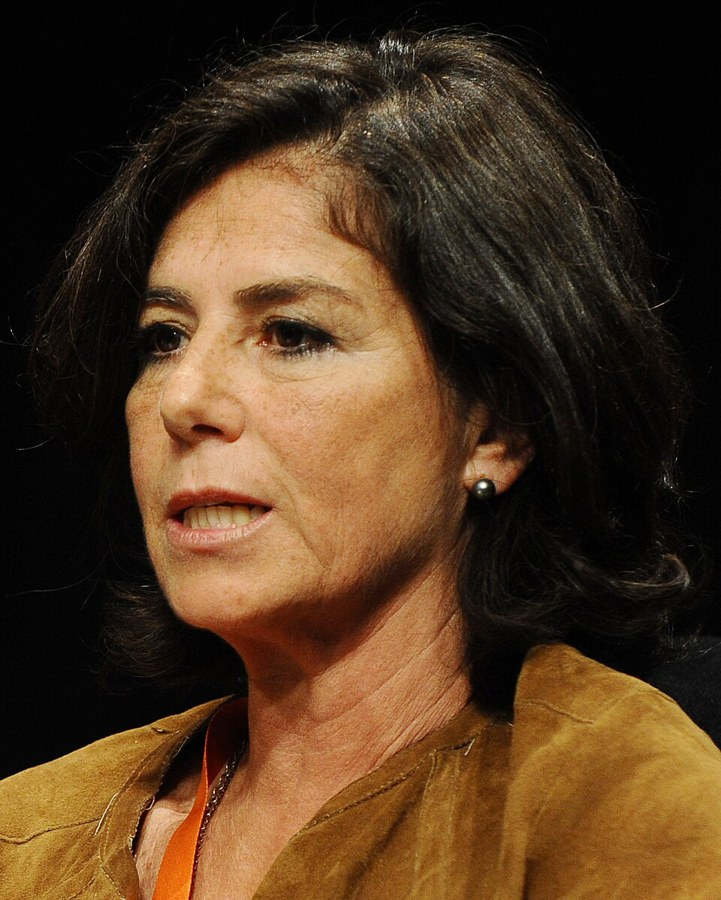
\includegraphics[height=0.34\textheight]{ch5_reichlin_2013.jpg}\\[1mm]
\imgcap{Lucrezia Reichlin, 2013}
\imgcredit{https://commons.wikimedia.org/wiki/File:Lucrezia_Reichlin_-_Festival_Economia_2013_(cropped).JPG}{Photo: Niccolò Caranti (2013); CC BY-SA 3.0; Wikimedia Commons}
\end{column}
\begin{column}{0.66\textwidth}
\begin{itemize}
    \item \textbf{Nowcasting}: estimating the present and the recent past of a low-frequency variable (GDP) from timelier high-frequency data \refGRS, \refBGMR
    \begin{itemize}
        \item backcast (last quarter, not yet published), nowcast (this quarter), forecast (next quarter)
    \end{itemize}
    \item Three difficulties: mixed frequencies, many indicators, asynchronous releases (the ragged edge)
    \begin{itemize}
        \item surveys are out at the end of the month; industrial production more than a month later; GDP weeks after the quarter
    \end{itemize}
    \item Tools: bridge equations \refBGP, MIDAS \refGSV, \refGSVb, mixed-frequency DFM \refMM, \refBM{} and mixed-frequency VARs \refSS
\end{itemize}
\end{column}
\end{columns}
\end{frame}

\begin{frame}{Bridge equations and MIDAS}
\itemsize{\small}
\begin{itemize}
    \item \textbf{Bridge}: forecast the missing months of each indicator (AR), aggregate to the quarter, regress GDP on the quarterly aggregates \refBGP
    \begin{itemize}
        \item simple and transparent; the error of the monthly AR forecasts passes into the nowcast
    \end{itemize}
    \item \textbf{MIDAS} \refGSV: $y_\tau = \beta_0 + \beta_1\sum_{j=0}^{K-1}w_j(\theta)x_{m_\tau - j} + \rho y_{\tau - s} + \varepsilon_\tau$, with the latest monthly value $x_{m_\tau}$
    \begin{itemize}
        \item $\tau$: the quarter; $m_\tau$: its latest available month; $x$: a monthly indicator with $K$ lags; $w_j(\theta)$: weights summing to 1; $y_{\tau - s}$: lagged GDP growth
        \item exponential Almon: $w_j(\theta) = e^{\theta_1j + \theta_2j^2}/\sum_ke^{\theta_1k + \theta_2k^2}$; two parameters for $K$ lags, estimated by NLS
        \item MIDAS with leads \refAGK, \refCG: one regression per information set; U-MIDAS leaves $w_j$ unrestricted when $K$ is small \refFMS
    \end{itemize}
    \item Neither uses the joint dynamics of the indicators; the DFM does
\end{itemize}
\end{frame}

\begin{frame}{Linking months and quarters: Mariano and Murasawa (2003)}
\itemsize{\small}
\begin{itemize}
    \item Let $Y_t^M$ be a latent monthly level and the quarterly GDP the 3-month average, observed in the third month
    \begin{itemize}
        \item geometric-mean approximation: $\ln Y_t^Q \approx \frac13(\ln Y_t^M + \ln Y_{t-1}^M + \ln Y_{t-2}^M)$
        \item quarterly growth $y_t^Q = \ln Y_t^Q - \ln Y_{t-3}^Q = \frac13(y_t + 2y_{t-1} + 3y_{t-2} + 2y_{t-3} + y_{t-4})$, $y_t$ = monthly growth \refMM
    \end{itemize}
    \item In the DFM: $y_t^Q = \lambda_y'\sum_{j=0}^{4}w_jf_{t-j} + e_t^Q$, $w = (1, 2, 3, 2, 1)/3$: the state must hold five lags of $f_t$
    \begin{itemize}
        \item $\lambda_y$: the loadings of GDP growth; $w_j$: the Mariano--Murasawa weights; $e_t^Q$: the idiosyncratic error of GDP
        \item GDP is a monthly variable observed every third month: missing in months 1 and 2 of each quarter
    \end{itemize}
    \item Seminar 5, A7: the weights by hand
\end{itemize}
\end{frame}

\begin{frame}{Case study: nowcasting Romanian GDP}
\itemsize{\footnotesize}
\begin{columns}[T]
\begin{column}{0.34\textwidth}
\centering
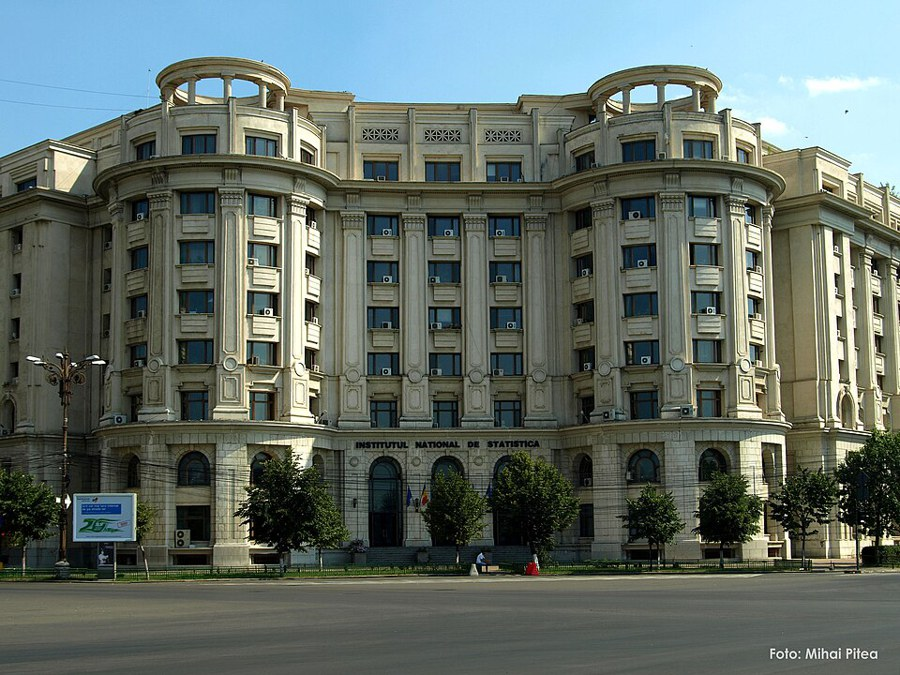
\includegraphics[height=0.3\textheight]{ch5_ins_bucharest_2009.jpg}\\[1mm]
\imgcap{Institutul Național de Statistică, Bucharest}
\imgcredit{https://commons.wikimedia.org/wiki/File:Institutul_Național_de_Statistică.jpg}{Photo: Dan Mihai Pitea (2009); CC BY-SA 3.0; Wikimedia Commons}
\end{column}
\begin{column}{0.64\textwidth}
\begin{itemize}
    \item Target: q/q growth of real GDP (Eurostat), 94 quarters to 2026Q2; monthly panel: 11 series from 2003 (Eurostat)
    \begin{itemize}
        \item hard data in monthly growth: IP, retail, construction, euro-area IP; change of unemployment; levels of six confidence balances
    \end{itemize}
    \item Stylised release lags at the end of each month: surveys 0, unemployment 1, hard data 2 months; GDP 2 months after the quarter
    \begin{itemize}
        \item current-vintage data: pseudo real time (no revisions)
    \end{itemize}
    \item Models: AR(1), bridge (IP, retail, ESI), MIDAS (IP, ESI; $K = 6$), DFM with two factors (two-step and EM)
\end{itemize}
\end{column}
\end{columns}
\end{frame}

\begin{frame}{Romanian GDP and two monthly indicators}
\itemsize{\footnotesize}
\begin{center}
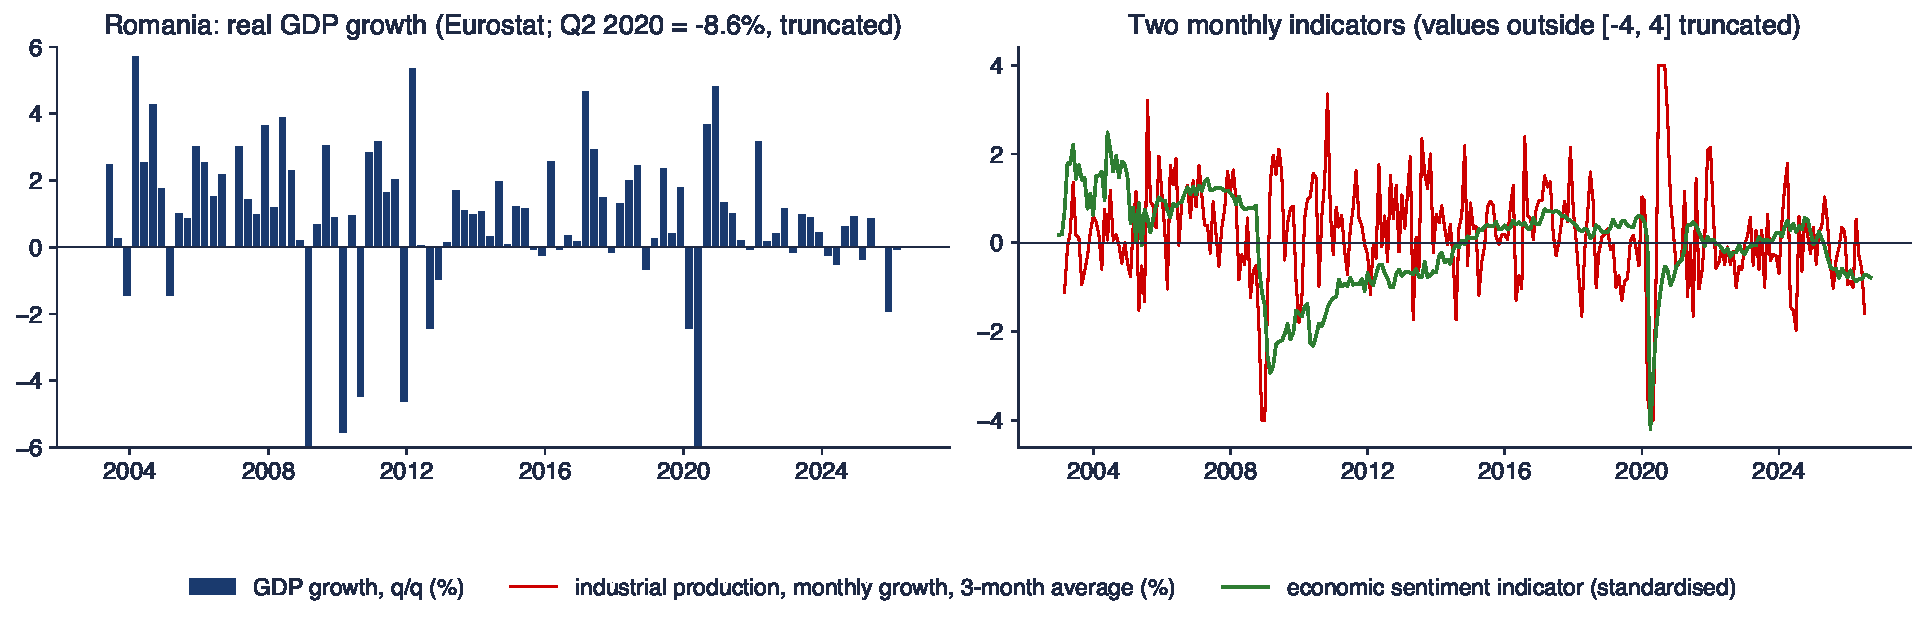
\includegraphics[width=0.97\textwidth,height=0.5\textheight,keepaspectratio]{ats_ch5_ro_data.pdf}
\end{center}
\vspace{-0.25cm}
\begin{itemize}
    \item Quarterly GDP growth (2020Q2: \ensuremath{-}8.6\%, truncated); IP growth (3-month average) and the standardised ESI
\end{itemize}
\quantlet{ATS\_ch5\_nowcast}{\qlurl{ATS_ch5_nowcast}}
\end{frame}

\begin{frame}{Interpreting the Romanian data}
\itemsize{\small}
\begin{itemize}
    \item Quarterly growth is volatile: 2009--2012 swings of $\pm 5$ pp and the 2020 collapse dominate the variance
    \item The ESI (3-month average) has correlation 0.44 with GDP growth before 2020: informative, far from perfect
    \item Latest published quarter: 2026Q2, growth 0.00\%; the nowcast target is 2026Q3
\end{itemize}
\end{frame}

\begin{frame}{MIDAS weights for Romania}
\itemsize{\footnotesize}
\begin{center}
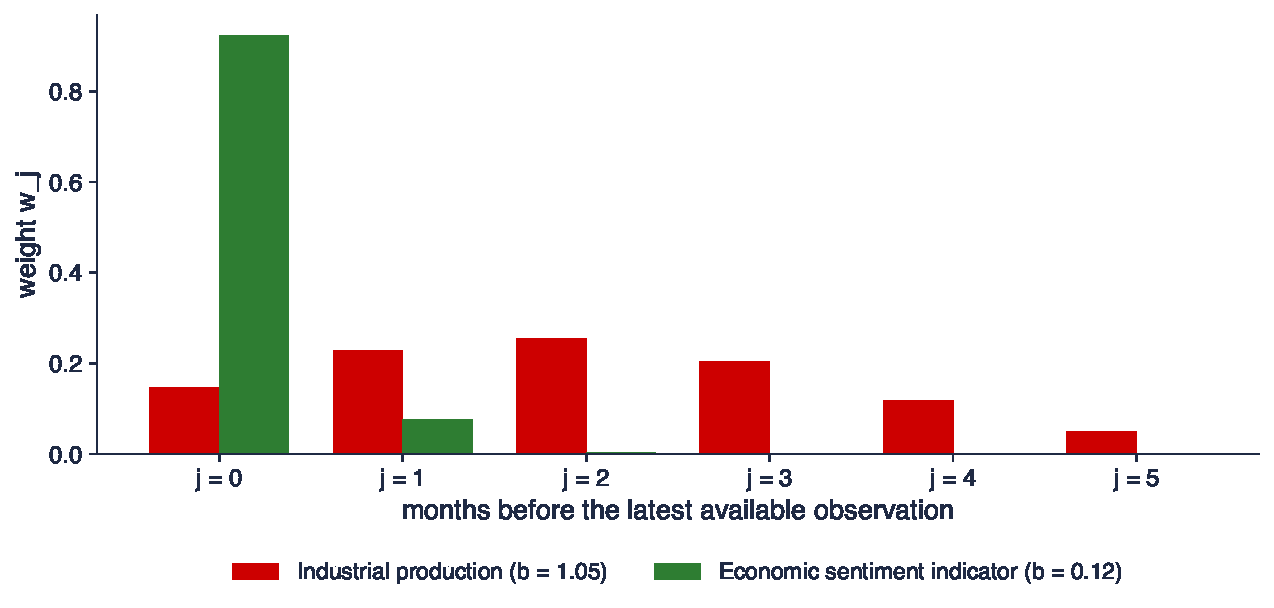
\includegraphics[width=0.97\textwidth,height=0.48\textheight,keepaspectratio]{ats_ch5_midas.pdf}
\end{center}
\vspace{-0.25cm}
\begin{itemize}
    \item ADL-MIDAS with exponential Almon weights at the end of the third month of the quarter, 2003--2026
\end{itemize}
\quantlet{ATS\_ch5\_nowcast}{\qlurl{ATS_ch5_nowcast}}
\end{frame}

\begin{frame}{Interpreting the MIDAS weights}
\itemsize{\small}
\begin{itemize}
    \item IP: hump-shaped weights peaking at lag 2 (0.25): the months of the quarter itself matter, as the Mariano--Murasawa weights predict
    \item ESI: weight 0.92 on the latest month: a level indicator already summarises the past
    \item Lagged GDP growth has coefficient \ensuremath{-}0.28: the noisy q/q series mean-reverts
\end{itemize}
\end{frame}

\begin{frame}{Pseudo-real-time evaluation}
\itemsize{\small}
\begin{itemize}
    \item For each quarter 2013Q1--2026Q2, nowcasts at the ends of months 1, 2, 3 of the quarter and of month 1 after it
    \begin{itemize}
        \item all parameters re-estimated on the data available at that date; 2020Q2--Q3 excluded from the RMSE (also reported with them)
    \end{itemize}
    \item The evaluation sample starts in 2013 because the 2009--2012 swings are larger than any model error; from 2010 the RMSEs rise to about 2 pp for every model
    \begin{itemize}
        \item standard deviation of the target 2013--2026 (without 2020Q2--Q3): 1.33 pp
    \end{itemize}
    \item Question: does the RMSE fall as the quarter unfolds, and by how much relative to an AR?
\end{itemize}
\end{frame}

\begin{frame}{Nowcast accuracy by information set}
\itemsize{\footnotesize}
\begin{center}
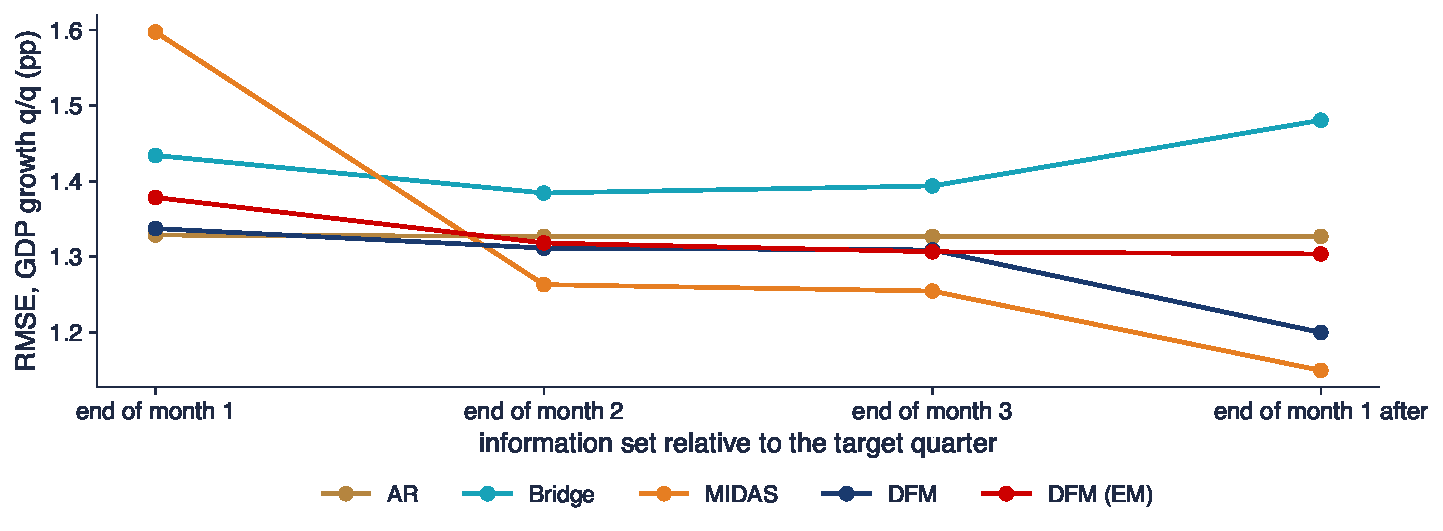
\includegraphics[width=0.97\textwidth,height=0.5\textheight,keepaspectratio]{ats_ch5_nowcast.pdf}
\end{center}
\vspace{-0.25cm}
\begin{itemize}
    \item RMSE of the nowcasts of q/q GDP growth, 2013Q1--2026Q2 without 2020Q2--Q3
\end{itemize}
\quantlet{ATS\_ch5\_nowcast}{\qlurl{ATS_ch5_nowcast}}
\end{frame}

\begin{frame}{Interpreting the nowcast accuracy}
\itemsize{\small}
\begin{itemize}
    \item AR: 1.33 pp throughout; DFM: 1.34 (month 1) to 1.20 (month 1 after); MIDAS: 1.60 to 1.15
    \item Bridge does not beat the AR (1.39); the EM estimate of the DFM is close to the AR (1.31 at month 3)
    \item Diebold--Mariano DFM against AR at month 3: $t = \ensuremath{-}0.30$, $p = 0.76$: the gain is not significant on 54 quarters
    \item With 2020: AR 1.90, DFM 1.30 at month 1 after: the monthly data catch the collapse, the AR cannot
\end{itemize}
\end{frame}

\begin{frame}{News and revisions: Bańbura and Modugno (2014)}
\itemsize{\small}
\begin{itemize}
    \item Information sets $\Omega_v \subset \Omega_{v+1}$; the new releases $x_j$, $j \in J_{v+1}$; the \textbf{news} is $I_j = x_j - \E[x_j\mid\Omega_v]$, not $x_j$
    \begin{itemize}
        \item with fixed parameters the revision of the nowcast of $y$ is a weighted sum of the news: $\E[y\mid\Omega_{v+1}] - \E[y\mid\Omega_v] = \E[yI']\E[II']^{-1}I = \sum_j w_jI_j$ \refBM
        \item $I$: the vector of news $I_j$; $w_j$: the weight of release $j$
    \end{itemize}
    \item In the DFM: $I_j = \lambda_j'(f_{t_j} - \hat f_{t_j\mid v}) + e_j$, so $\E[II'] = H P_{\mid v}H' + \Psi_J$ and $\E[yI'] = z_y'P_{\mid v}H'$
    \begin{itemize}
        \item $\lambda_j$: the loadings of release $j$; $t_j$: its reference month; $\hat f_{t_j\mid v}$: the factor estimate given $\Omega_v$; $H$: the stacked $\lambda_j'$; $\Psi_J$: their idiosyncratic variances; $z_y$: the loading of the target
        \item $P_{\mid v}$: the covariance of the stacked state given $\Omega_v$, from the Kalman filter
    \end{itemize}
    \item A large release that was expected moves nothing; a small surprise in a heavily weighted series moves a lot; correlated releases share their weight
\end{itemize}
\end{frame}

\begin{frame}{Nowcasting 2026Q3, and where the revision came from}
\itemsize{\footnotesize}
\begin{center}
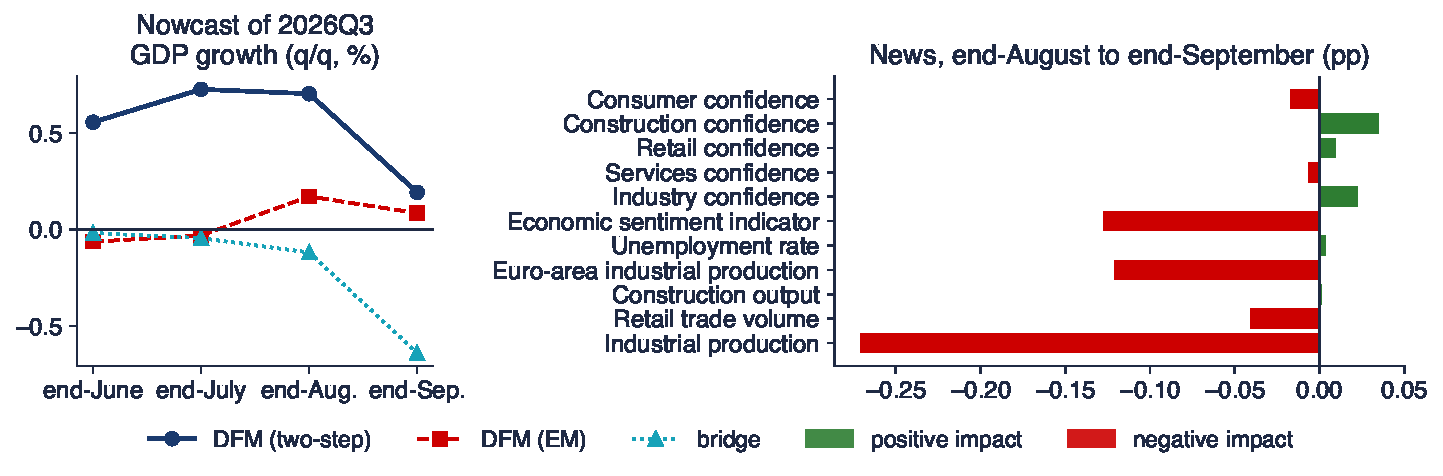
\includegraphics[width=0.97\textwidth,height=0.5\textheight,keepaspectratio]{ats_ch5_news.pdf}
\end{center}
\vspace{-0.25cm}
\begin{itemize}
    \item Left: nowcasts at the ends of June--September 2026; right: news decomposition of the two-step DFM nowcast between the August and September information sets
\end{itemize}
\quantlet{ATS\_ch5\_nowcast}{\qlurl{ATS_ch5_nowcast}}
\end{frame}

\begin{frame}{Interpreting the news}
\itemsize{\small}
\begin{itemize}
    \item DFM nowcast of 2026Q3: 0.70\% at the end of August, 0.19\% at the end of September; the 11 new releases add up to \ensuremath{-}0.51 pp exactly
    \item The July IP release was \ensuremath{-}3.7 pp below the model's expectation; with weight 0.073 it cut the nowcast by \ensuremath{-}0.27 pp; ESI \ensuremath{-}0.13, euro-area IP \ensuremath{-}0.12
    \item Other models at the end of September: EM DFM 0.08\%, bridge \ensuremath{-}0.64\%, AR 0.76\%: the first official estimate for 2026Q3 will judge them
    \item The news decomposition turns a number into a story that a central bank can check release by release
\end{itemize}
\end{frame}

\begin{frame}{Recap: Nowcasting}
\itemsize{\small}
\begin{itemize}
    \item Nowcasting = filtering a mixed-frequency system with a ragged edge
    \item Bridge, MIDAS and DFM share the Mariano--Murasawa link between months and quarters
    \item For Romania, monthly data improve the nowcast late in the quarter; the gain is modest and not significant
    \item Every revision decomposes exactly into news with fixed parameters
\end{itemize}
\end{frame}


%=============================================================================
\section{AI for scientific discovery}
%=============================================================================

\begin{frame}{An open question}
\itemsize{\small}
\begin{itemize}
    \item Can a nowcasting model beat a simple AR for Romanian GDP growth in a statistically significant way, and which releases carry the information?
    \begin{itemize}
        \item formal: $H_0$: equal MSE of the DFM and AR nowcasts at the end of month 3 (Diebold--Mariano, \atschlink{https://danpele.github.io/Advanced-Time-Series/EN/Courses/chapter1_forecast_evaluation.pdf}{Chapter 1}), pre-registered sample, models and lags
        \item falsified by a rejection on quarters the model never saw, with real-time vintages of GDP
    \end{itemize}
    \item Why it matters: fiscal and monetary decisions in 2025--2026 were taken with GDP known only weeks after each quarter
    \begin{itemize}
        \item literature to start from: \refGRS, \refBM, \refBGMR, \refGLPb, \refSS
    \end{itemize}
\end{itemize}
\end{frame}

\begin{frame}{The discovery loop with an AI assistant}
\itemsize{\footnotesize}
\begin{itemize}
    \item An AI assistant (an LLM such as Claude, ChatGPT, Gemini or Copilot) speeds up each step; Semantic Scholar and Elicit help with the literature
    \begin{itemize}
        \item \textbf{literature}: \aiprompt{List peer-reviewed papers that nowcast GDP of Central and Eastern European countries with factor models or MIDAS; give DOIs.} Then check every DOI on Crossref
        \item \textbf{hypothesis}: \aiprompt{Which Romanian monthly releases should carry news about GDP, and in which month of the quarter?}
        \item \textbf{code and replication}: ask for a Kalman filter with missing data, then reproduce a known number first (the news sum of this lecture)
        \item \textbf{robustness and critique}: \aiprompt{Act as a hostile referee of a nowcasting paper: list the ways the pseudo-real-time design could flatter the model.}
    \end{itemize}
    \item Report: what was asked, what was kept, what was rejected (AI\_USE.md, AI\_ERRORS.md)
\end{itemize}
\end{frame}

\begin{frame}{What the human checks}
\itemsize{\small}
\begin{itemize}
    \item Every reference exists and says what is claimed (DOI resolves, title matches, the result is in the paper)
    \item The information set at each date contains only data published by then; current-vintage data overstate accuracy
    \item Hyperparameters, factors and lags are chosen inside each estimation window, never on the evaluation sample
    \item The evaluation period and the treatment of 2020 are fixed before the results; all variants are reported
    \item A claim of ``better nowcasts'' is backed by a test, not by a lower RMSE alone
\end{itemize}
\end{frame}

\begin{frame}{Mini-case: how robust is one ranking?}
\itemsize{\footnotesize}
\begin{center}
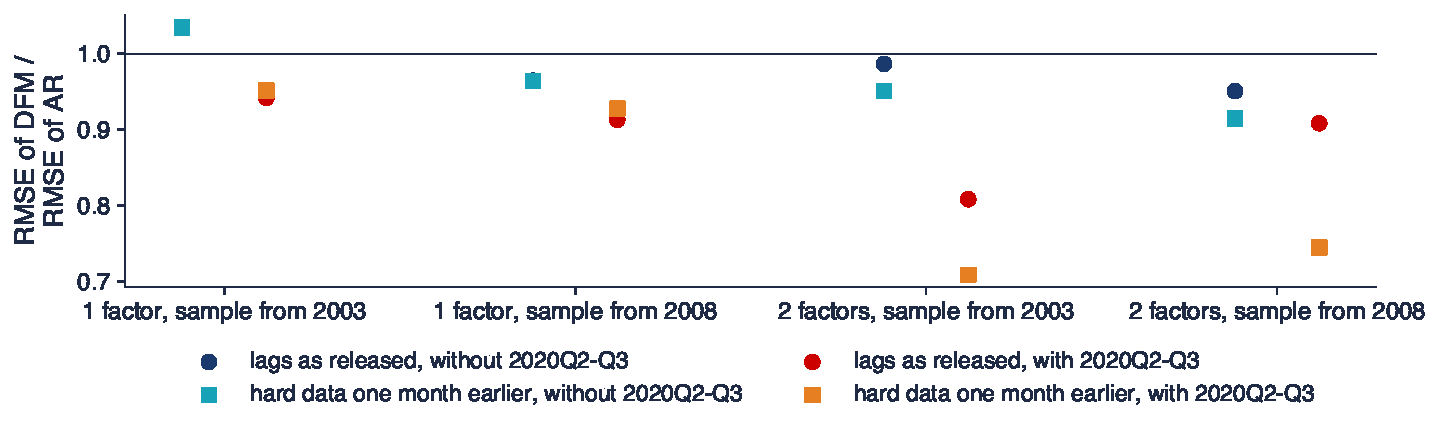
\includegraphics[width=0.97\textwidth,height=0.48\textheight,keepaspectratio]{ats_ch5_ai_case.pdf}
\end{center}
\vspace{-0.25cm}
\begin{itemize}
    \item RMSE of the DFM nowcast relative to the AR at the end of month 3, 2013--2026, across factors, sample start, release lags and the treatment of 2020
    \item 16 variants range from 0.71 to 1.03; the DFM wins in 14 of them: an AI summary that reports the best variant as ``the'' result is wrong
\end{itemize}
\quantlet{ATS\_ch5\_nowcast}{\qlurl{ATS_ch5_nowcast}}
\end{frame}

\begin{frame}{Project idea}
\itemsize{\small}
\begin{itemize}
    \item \textbf{A real-time nowcasting model for Romanian GDP}: replicate first, then extend
    \begin{itemize}
        \item replicate: the news decomposition of this lecture (\ensuremath{-}0.51 pp between August and September 2026) and the BGR table for 1971--2003
        \item extend: real release dates (INS calendar), GDP vintages saved from now on, blocks of factors for hard and soft data, a mixed-frequency BVAR, density nowcasts
        \item pre-register: target, quarters, models, information sets, the treatment of 2020 and the Diebold--Mariano test
    \end{itemize}
    \item Deliverables follow the course rules: repository, report, AI\_USE.md, AI\_ERRORS.md, oral defence
\end{itemize}
\end{frame}


%=============================================================================
\section{Wrap-up}
%=============================================================================

\begin{frame}{Key takeaways}
\itemsize{\small}
\begin{itemize}
    \item Many series and few observations: shrink (priors) or compress (factors)
    \item The Minnesota prior in conjugate form gives closed-form posteriors, exact draws and a marginal likelihood that chooses the shrinkage
    \item Bigger systems need tighter priors; then they forecast better and give more plausible responses
    \item Principal components estimate the factor space; Bai--Ng chooses its dimension; FAVAR and DFM put it to work
    \item Nowcasting is Kalman filtering with a ragged edge; every revision is a sum of news
\end{itemize}
\end{frame}

\begin{frame}{Self-assessment}
\itemsize{\small}
\begin{columns}[T]
\begin{column}{0.56\textwidth}
\begin{block}{Questions}
\begin{itemize}
    \item What happens to the Minnesota posterior mean when $\lambda \to 0$?
    \item Why does the natural conjugate prior force $\vartheta = 1$?
    \item Which prior allows cointegration: sum-of-coefficients or initial observation?
    \item Why can PCA identify only the factor space?
    \item Why is a large but expected release not news?
\end{itemize}
\end{block}
\end{column}
\begin{column}{0.40\textwidth}
\begin{block}{Next: \atschlink{https://danpele.github.io/Advanced-Time-Series/EN/Courses/chapter6_state_space_models_bayesian_filtering.pdf}{Chapter 6}}
\begin{itemize}
    \item State space models and Bayesian filtering
    \item The Kalman filter and smoother in full; EM, particle filters, stochastic volatility
\end{itemize}
\end{block}
\end{column}
\end{columns}
\end{frame}


%=============================================================================
\section{Appendix}
%=============================================================================

\begin{frame}{Appendix: the natural conjugate posterior}
\hypertarget{atsapp1}{}\atsappback{atssrc1}{Back}
\itemsize{\small}
\begin{itemize}
    \item Likelihood: $p(Y\mid B, \Sigma) \propto |\Sigma|^{-T/2}\exp\{-\frac12\mathrm{tr}[\Sigma^{-1}(Y - XB)'(Y - XB)]\}$
    \item Prior: $|\Sigma|^{-k/2}\exp\{-\frac12\mathrm{tr}[\Sigma^{-1}(B - B_0)'\Omega_0^{-1}(B - B_0)]\}\times|\Sigma|^{-(d + n + 1)/2}\exp\{-\frac12\mathrm{tr}(\Sigma^{-1}\Psi)\}$
    \item Complete the square in $B$: $(Y - XB)'(Y - XB) + (B - B_0)'\Omega_0^{-1}(B - B_0) = (B - \bar B)'\bar\Omega^{-1}(B - \bar B) + \hat U'\hat U + (\bar B - B_0)'\Omega_0^{-1}(\bar B - B_0)$
    \item Hence $B\mid\Sigma, Y \sim MN(\bar B, \bar\Omega, \Sigma)$ and $\Sigma\mid Y \sim IW(\bar\Psi, T + d)$: the same families as the prior
\end{itemize}
\end{frame}

\begin{frame}{Appendix: the marginal likelihood in closed form}
\hypertarget{atsapp2}{}\atsappback{atssrc1}{Back}
\itemsize{\small}
\begin{itemize}
    \item Integrating $B$ and $\Sigma$ out (GLP, appendix): $p(Y) = \pi^{-nT/2}\frac{\Gamma_n(\frac{T + d}2)}{\Gamma_n(\frac d2)}|\Omega_0|^{-\frac n2}|X'X + \Omega_0^{-1}|^{-\frac n2}|\Psi|^{\frac d2}|\bar\Psi|^{-\frac{T + d}2}$
    \item $|\Omega_0|\,|X'X + \Omega_0^{-1}| = |I + \Omega_0X'X|$: the complexity penalty, growing with $\lambda$
    \item $|\bar\Psi|$: the fit term, falling with $\lambda$; the optimum balances the two
    \item With dummies: $\ln p(Y\mid\gamma) = \ln p(Y, Y_d\mid\gamma) - \ln p(Y_d\mid\gamma)$, each by the formula above
\end{itemize}
\end{frame}


%=============================================================================
\section{References}
%=============================================================================

\begin{frame}{References (1/5)}
\itemsize{\tiny}
\begin{itemize}
    \item Andreou, E., Ghysels, E., \& Kourtellos, A. (2013). Should macroeconomic forecasters use daily financial data and how? \textit{Journal of Business \& Economic Statistics}, 31(2), 240--251. \href{https://doi.org/10.1080/07350015.2013.767199}{doi:10.1080/07350015.2013.767199}
    \item Aruoba, S. B., Diebold, F. X., \& Scotti, C. (2009). Real-time measurement of business conditions. \textit{Journal of Business \& Economic Statistics}, 27(4), 417--427. \href{https://doi.org/10.1198/jbes.2009.07205}{doi:10.1198/jbes.2009.07205}
    \item Bańbura, M., Giannone, D., Modugno, M., \& Reichlin, L. (2013). Now-casting and the real-time data flow. In G. Elliott \& A. Timmermann (Eds.), \textit{Handbook of Economic Forecasting} (Vol.\ 2A, pp.\ 195--237). Elsevier. \href{https://doi.org/10.1016/B978-0-444-53683-9.00004-9}{doi:10.1016/B978-0-444-53683-9.00004-9}
    \item Bańbura, M., Giannone, D., \& Reichlin, L. (2010). Large Bayesian vector auto regressions. \textit{Journal of Applied Econometrics}, 25(1), 71--92. \href{https://doi.org/10.1002/jae.1137}{doi:10.1002/jae.1137}
    \item Bańbura, M., \& Modugno, M. (2014). Maximum likelihood estimation of factor models on datasets with arbitrary pattern of missing data. \textit{Journal of Applied Econometrics}, 29(1), 133--160. \href{https://doi.org/10.1002/jae.2306}{doi:10.1002/jae.2306}
    \item Baffigi, A., Golinelli, R., \& Parigi, G. (2004). Bridge models to forecast the euro area GDP. \textit{International Journal of Forecasting}, 20(3), 447--460. \href{https://doi.org/10.1016/S0169-2070(03)00067-0}{doi:10.1016/S0169-2070(03)00067-0}
    \item Bai, J. (2003). Inferential theory for factor models of large dimensions. \textit{Econometrica}, 71(1), 135--171. \href{https://doi.org/10.1111/1468-0262.00392}{doi:10.1111/1468-0262.00392}
    \item Bai, J., \& Ng, S. (2002). Determining the number of factors in approximate factor models. \textit{Econometrica}, 70(1), 191--221. \href{https://doi.org/10.1111/1468-0262.00273}{doi:10.1111/1468-0262.00273}
    \item Bernanke, B. S., Boivin, J., \& Eliasz, P. (2005). Measuring the effects of monetary policy: A factor-augmented vector autoregressive (FAVAR) approach. \textit{The Quarterly Journal of Economics}, 120(1), 387--422. \href{https://doi.org/10.1162/0033553053327452}{doi:10.1162/0033553053327452}
    \item Carriero, A., Clark, T. E., \& Marcellino, M. (2016). Common drifting volatility in large Bayesian VARs. \textit{Journal of Business \& Economic Statistics}, 34(3), 375--390. \href{https://doi.org/10.1080/07350015.2015.1040116}{doi:10.1080/07350015.2015.1040116}
    \item Carriero, A., Clark, T. E., \& Marcellino, M. (2019). Large Bayesian vector autoregressions with stochastic volatility and non-conjugate priors. \textit{Journal of Econometrics}, 212(1), 137--154. \href{https://doi.org/10.1016/j.jeconom.2019.04.024}{doi:10.1016/j.jeconom.2019.04.024}
    \item Chamberlain, G., \& Rothschild, M. (1983). Arbitrage, factor structure, and mean-variance analysis on large asset markets. \textit{Econometrica}, 51(5), 1281--1304. \href{https://doi.org/10.2307/1912275}{doi:10.2307/1912275}
\end{itemize}
\end{frame}

\begin{frame}{References (2/5)}
\itemsize{\tiny}
\begin{itemize}
    \item Chan, J. C. C. (2020). Large Bayesian vector autoregressions. In P. Fuleky (Ed.), \textit{Macroeconomic Forecasting in the Era of Big Data} (pp.\ 95--125). Springer. \href{https://doi.org/10.1007/978-3-030-31150-6_4}{doi:10.1007/978-3-030-31150-6\_4}
    \item Clark, T. E. (2011). Real-time density forecasts from Bayesian vector autoregressions with stochastic volatility. \textit{Journal of Business \& Economic Statistics}, 29(3), 327--341. \href{https://doi.org/10.1198/jbes.2010.09248}{doi:10.1198/jbes.2010.09248}
    \item Clements, M. P., \& Galvão, A. B. (2008). Macroeconomic forecasting with mixed-frequency data: Forecasting output growth in the United States. \textit{Journal of Business \& Economic Statistics}, 26(4), 546--554. \href{https://doi.org/10.1198/073500108000000015}{doi:10.1198/073500108000000015}
    \item Croushore, D., \& Stark, T. (2001). A real-time data set for macroeconomists. \textit{Journal of Econometrics}, 105(1), 111--130. \href{https://doi.org/10.1016/S0304-4076(01)00072-0}{doi:10.1016/S0304-4076(01)00072-0}
    \item De Mol, C., Giannone, D., \& Reichlin, L. (2008). Forecasting using a large number of predictors: Is Bayesian shrinkage a valid alternative to principal components? \textit{Journal of Econometrics}, 146(2), 318--328. \href{https://doi.org/10.1016/j.jeconom.2008.08.011}{doi:10.1016/j.jeconom.2008.08.011}
    \item Doan, T., Litterman, R., \& Sims, C. (1984). Forecasting and conditional projection using realistic prior distributions. \textit{Econometric Reviews}, 3(1), 1--100. \href{https://doi.org/10.1080/07474938408800053}{doi:10.1080/07474938408800053}
    \item Doz, C., Giannone, D., \& Reichlin, L. (2012). A quasi-maximum likelihood approach for large, approximate dynamic factor models. \textit{The Review of Economics and Statistics}, 94(4), 1014--1024. \href{https://doi.org/10.1162/REST_a_00225}{doi:10.1162/REST\_a\_00225}
    \item Doz, C., Giannone, D., \& Reichlin, L. (2011). A two-step estimator for large approximate dynamic factor models based on Kalman filtering. \textit{Journal of Econometrics}, 164(1), 188--205. \href{https://doi.org/10.1016/j.jeconom.2011.02.012}{doi:10.1016/j.jeconom.2011.02.012}
    \item Durbin, J., \& Koopman, S. J. (2012). \textit{Time Series Analysis by State Space Methods} (2nd ed.). Oxford University Press. \href{https://doi.org/10.1093/acprof:oso/9780199641178.001.0001}{doi:10.1093/acprof:oso/9780199641178.001.0001}
    \item Forni, M., Hallin, M., Lippi, M., \& Reichlin, L. (2000). The generalized dynamic-factor model: Identification and estimation. \textit{The Review of Economics and Statistics}, 82(4), 540--554. \href{https://doi.org/10.1162/003465300559037}{doi:10.1162/003465300559037}
    \item Foroni, C., Marcellino, M., \& Schumacher, C. (2015). Unrestricted mixed data sampling (MIDAS): MIDAS regressions with unrestricted lag polynomials. \textit{Journal of the Royal Statistical Society: Series A}, 178(1), 57--82. \href{https://doi.org/10.1111/rssa.12043}{doi:10.1111/rssa.12043}
    \item Gelfand, A. E., \& Smith, A. F. M. (1990). Sampling-based approaches to calculating marginal densities. \textit{Journal of the American Statistical Association}, 85(410), 398--409. \href{https://doi.org/10.1080/01621459.1990.10476213}{doi:10.1080/01621459.1990.10476213}
\end{itemize}
\end{frame}

\begin{frame}{References (3/5)}
\itemsize{\tiny}
\begin{itemize}
    \item Gelman, A., Carlin, J. B., Stern, H. S., Dunson, D. B., Vehtari, A., \& Rubin, D. B. (2013). \textit{Bayesian Data Analysis} (3rd ed.). Chapman and Hall/CRC. \href{https://doi.org/10.1201/b16018}{doi:10.1201/b16018}
    \item Gelman, A., \& Rubin, D. B. (1992). Inference from iterative simulation using multiple sequences. \textit{Statistical Science}, 7(4), 457--472. \href{https://doi.org/10.1214/ss/1177011136}{doi:10.1214/ss/1177011136}
    \item Geman, S., \& Geman, D. (1984). Stochastic relaxation, Gibbs distributions, and the Bayesian restoration of images. \textit{IEEE Transactions on Pattern Analysis and Machine Intelligence}, PAMI-6(6), 721--741. \href{https://doi.org/10.1109/TPAMI.1984.4767596}{doi:10.1109/TPAMI.1984.4767596}
    \item Ghysels, E. (2016). Macroeconomics and the reality of mixed frequency data. \textit{Journal of Econometrics}, 193(2), 294--314. \href{https://doi.org/10.1016/j.jeconom.2016.04.008}{doi:10.1016/j.jeconom.2016.04.008}
    \item Ghysels, E., Santa-Clara, P., \& Valkanov, R. (2006). Predicting volatility: Getting the most out of return data sampled at different frequencies. \textit{Journal of Econometrics}, 131(1--2), 59--95. \href{https://doi.org/10.1016/j.jeconom.2005.01.004}{doi:10.1016/j.jeconom.2005.01.004}
    \item Ghysels, E., Sinko, A., \& Valkanov, R. (2007). MIDAS regressions: Further results and new directions. \textit{Econometric Reviews}, 26(1), 53--90. \href{https://doi.org/10.1080/07474930600972467}{doi:10.1080/07474930600972467}
    \item Giannone, D., Lenza, M., \& Primiceri, G. E. (2021). Economic predictions with big data: The illusion of sparsity. \textit{Econometrica}, 89(5), 2409--2437. \href{https://doi.org/10.3982/ECTA17842}{doi:10.3982/ECTA17842}
    \item Giannone, D., Lenza, M., \& Primiceri, G. E. (2015). Prior selection for vector autoregressions. \textit{The Review of Economics and Statistics}, 97(2), 436--451. \href{https://doi.org/10.1162/REST_a_00483}{doi:10.1162/REST\_a\_00483}
    \item Giannone, D., Reichlin, L., \& Small, D. (2008). Nowcasting: The real-time informational content of macroeconomic data. \textit{Journal of Monetary Economics}, 55(4), 665--676. \href{https://doi.org/10.1016/j.jmoneco.2008.05.010}{doi:10.1016/j.jmoneco.2008.05.010}
    \item Hamilton, J. D. (1994). \textit{Time Series Analysis}. Princeton University Press. \href{https://doi.org/10.2307/j.ctv14jx6sm}{doi:10.2307/j.ctv14jx6sm}
    \item Kadiyala, K. R., \& Karlsson, S. (1997). Numerical methods for estimation and inference in Bayesian VAR-models. \textit{Journal of Applied Econometrics}, 12(2), 99--132. \href{https://doi.org/10.1002/(SICI)1099-1255(199703)12:2\%3C99::AID-JAE429\%3E3.0.CO;2-A}{doi:10.1002/(SICI)1099-1255(199703)12:2\textless{}99::AID-JAE429\textgreater{}3.0.CO;2-A}
    \item Karlsson, S. (2013). Forecasting with Bayesian vector autoregression. In G. Elliott \& A. Timmermann (Eds.), \textit{Handbook of Economic Forecasting} (Vol.\ 2B, pp.\ 791--897). Elsevier. \href{https://doi.org/10.1016/B978-0-444-62731-5.00015-4}{doi:10.1016/B978-0-444-62731-5.00015-4}
\end{itemize}
\end{frame}

\begin{frame}{References (4/5)}
\itemsize{\tiny}
\begin{itemize}
    \item Kass, R. E., \& Raftery, A. E. (1995). Bayes factors. \textit{Journal of the American Statistical Association}, 90(430), 773--795. \href{https://doi.org/10.1080/01621459.1995.10476572}{doi:10.1080/01621459.1995.10476572}
    \item Kilian, L., \& Lütkepohl, H. (2017). \textit{Structural Vector Autoregressive Analysis}. Cambridge University Press. \href{https://doi.org/10.1017/9781108164818}{doi:10.1017/9781108164818}
    \item Koop, G. (2013). Forecasting with medium and large Bayesian VARs. \textit{Journal of Applied Econometrics}, 28(2), 177--203. \href{https://doi.org/10.1002/jae.1270}{doi:10.1002/jae.1270}
    \item Koop, G., \& Korobilis, D. (2010). Bayesian multivariate time series methods for empirical macroeconomics. \textit{Foundations and Trends in Econometrics}, 3(4), 267--358. \href{https://doi.org/10.1561/0800000013}{doi:10.1561/0800000013}
    \item Lenza, M., \& Primiceri, G. E. (2022). How to estimate a vector autoregression after March 2020. \textit{Journal of Applied Econometrics}, 37(4), 688--699. \href{https://doi.org/10.1002/jae.2895}{doi:10.1002/jae.2895}
    \item Litterman, R. B. (1986). Forecasting with Bayesian vector autoregressions: Five years of experience. \textit{Journal of Business \& Economic Statistics}, 4(1), 25--38. \href{https://doi.org/10.1080/07350015.1986.10509491}{doi:10.1080/07350015.1986.10509491}
    \item Mariano, R. S., \& Murasawa, Y. (2003). A new coincident index of business cycles based on monthly and quarterly series. \textit{Journal of Applied Econometrics}, 18(4), 427--443. \href{https://doi.org/10.1002/jae.695}{doi:10.1002/jae.695}
    \item McCracken, M. W., \& Ng, S. (2016). FRED-MD: A monthly database for macroeconomic research. \textit{Journal of Business \& Economic Statistics}, 34(4), 574--589. \href{https://doi.org/10.1080/07350015.2015.1086655}{doi:10.1080/07350015.2015.1086655}
    \item Petropoulos, F., Apiletti, D., Assimakopoulos, V., Babai, M. Z., et al.\ (2022). Forecasting: Theory and practice. \textit{International Journal of Forecasting}, 38(3), 705--871. \href{https://doi.org/10.1016/j.ijforecast.2021.11.001}{doi:10.1016/j.ijforecast.2021.11.001}
    \item Primiceri, G. E. (2005). Time varying structural vector autoregressions and monetary policy. \textit{The Review of Economic Studies}, 72(3), 821--852. \href{https://doi.org/10.1111/j.1467-937X.2005.00353.x}{doi:10.1111/j.1467-937X.2005.00353.x}
    \item Schorfheide, F., \& Song, D. (2015). Real-time forecasting with a mixed-frequency VAR. \textit{Journal of Business \& Economic Statistics}, 33(3), 366--380. \href{https://doi.org/10.1080/07350015.2014.954707}{doi:10.1080/07350015.2014.954707}
    \item Sims, C. A. (1993). A nine-variable probabilistic macroeconomic forecasting model. In J. H. Stock \& M. W. Watson (Eds.), \textit{Business Cycles, Indicators and Forecasting} (pp.\ 179--212). University of Chicago Press. \href{https://www.nber.org/books-and-chapters/business-cycles-indicators-and-forecasting/nine-variable-probabilistic-macroeconomic-forecasting-model}{nber.org}
\end{itemize}
\end{frame}

\begin{frame}{References (5/5)}
\itemsize{\tiny}
\begin{itemize}
    \item Sims, C. A., \& Zha, T. (1998). Bayesian methods for dynamic multivariate models. \textit{International Economic Review}, 39(4), 949--968. \href{https://doi.org/10.2307/2527347}{doi:10.2307/2527347}
    \item Stock, J. H., \& Watson, M. W. (2002a). Forecasting using principal components from a large number of predictors. \textit{Journal of the American Statistical Association}, 97(460), 1167--1179. \href{https://doi.org/10.1198/016214502388618960}{doi:10.1198/016214502388618960}
    \item Stock, J. H., \& Watson, M. W. (2002b). Macroeconomic forecasting using diffusion indexes. \textit{Journal of Business \& Economic Statistics}, 20(2), 147--162. \href{https://doi.org/10.1198/073500102317351921}{doi:10.1198/073500102317351921}
    \item Stock, J. H., \& Watson, M. W. (2016). Dynamic factor models, factor-augmented vector autoregressions, and structural vector autoregressions in macroeconomics. In J. B. Taylor \& H. Uhlig (Eds.), \textit{Handbook of Macroeconomics} (Vol.\ 2A, pp.\ 415--525). Elsevier. \href{https://doi.org/10.1016/bs.hesmac.2016.04.002}{doi:10.1016/bs.hesmac.2016.04.002}
    \item Stock, J. H., \& Watson, M. W. (1989). New indexes of coincident and leading economic indicators. \textit{NBER Macroeconomics Annual}, 4, 351--394. \href{https://doi.org/10.1086/654119}{doi:10.1086/654119}
    \item Vehtari, A., Gelman, A., Simpson, D., Carpenter, B., \& Bürkner, P.-C. (2021). Rank-normalization, folding, and localization: An improved $\widehat{R}$ for assessing convergence of MCMC. \textit{Bayesian Analysis}, 16(2), 667--718. \href{https://doi.org/10.1214/20-BA1221}{doi:10.1214/20-BA1221}
\end{itemize}
\end{frame}

\end{document}
